\documentclass[12pt,a4paper,english,twoside]{book}
\usepackage[english,main=english]{babel} % I added main= before english,else  compiler complaint 
\usepackage[T1]{fontenc} 
\usepackage[utf8]{inputenc} % I changed from latin1 to utf8, else umlaute not displayed correctly
\usepackage{amsfonts}
\usepackage{amsmath}
\usepackage{latexsym}
\usepackage{amssymb}
\usepackage{epsfig}
\usepackage{moreverb}
\usepackage{rotating}
\usepackage{enumerate}
\usepackage{graphics, graphicx,wrapfig}
\usepackage{fancybox}
\usepackage{picinpar,varioref,floatflt}
\usepackage{ae}
\usepackage{longtable}
\usepackage{textcomp}
\usepackage{float}
\usepackage{url}
\usepackage{unizhdt}
\usepackage{csquotes}
\usepackage{markdown}
\usepackage{booktabs}
\usepackage{hyperref}
\usepackage{caption}
\usepackage{subcaption}
\usepackage{minted}
\usepackage{booktabs}
\usepackage{multirow}
\usepackage{array}
\usepackage{multirow}
\usepackage{siunitx}
\usepackage{graphicx}
\usepackage{listings}
\usepackage{color}






\definecolor{dkgreen}{rgb}{0,0.6,0}
\definecolor{gray}{rgb}{0.5,0.5,0.5}
\definecolor{mauve}{rgb}{0.58,0,0.82}
\lstset{frame=tb,
  language=Java,
  aboveskip=3mm,
  belowskip=3mm,
  showstringspaces=false,
  columns=flexible,
  basicstyle={\linespread{1.0}\small\ttfamily},
  numbers=none,
  numberstyle=\tiny\color{gray},
  keywordstyle=\color{blue},
  commentstyle=\color{dkgreen},
  stringstyle=\color{mauve},
  breaklines=true,
  breakatwhitespace=true,
  tabsize=3,
}

\linespread{1.5}

\usepackage[section]{placeins}





\usepackage[table]{xcolor}



\usepackage{tabularx}

\usepackage{longtable}% http://ctan.org/pkg/longtable
\usepackage{array,booktabs,enumitem}% http://ctan.org/pkg/{array,booktabs,enumitem}



\usepackage{makecell,multirow}
\renewcommand\theadfont{\bfseries\normalsize}
\usepackage{caption}
\usepackage{calc}
\usepackage{enumitem}














\providecommand{\tightlist}{%
  \setlength{\itemsep}{0pt}\setlength{\parskip}{0pt}}


\MakeOuterQuote{"}



%%%%%%%%%%%%%%%%%%%%%%%%%%%%%%%%%%%%%%%%%%%%%%%%%%

% Define the language of the diploma thesis
\selectlanguage{english}
%\selectlanguage{german}

\pagestyle{headings}

\begin{document}



%%%%%%%%%%%%%%%%%%%%%%%%%%%%%%%%%%%%%%%%%%%%%%%%%%

% Define the author printed on the cover page
\author{Elfat Esati}
% Define the city and country of the author
\authorcity{Zurich, Switzerland}
% Define the student ID (Matrikelnummer)
\studentid{15-702-103}
% Define the title with optional subtitle
\title{Tamper-resistant IoT based surveillance using blockchain technology}
% Define the supervisors
\supervisors{Eryk Schiller}
% Define the submission date
\submissiondate{January 30, 2021}

%%%%%%%%%%%%%%%%%%%%%%%%%%%%%%%%%%%%%%%%%%%%%%%%%%

% Make the title page
\maketitle

% Make the imprint on the back of the cover page
\makeimprint

\pagenumbering{roman}

% Include the files of the diploma thesis
%\cleardoublepage
\chapter*{Abstract}
\addcontentsline{toc}{chapter}{Abstract}


\selectlanguage{english}

The Internet of Things (IoT), artificial
intelligence (AI), and blockchain are one of the most disruptive technologies that scholars have begun evaluating. In one hand blockchain technology as a distributed  decentralized peer to peer network promises to keep  records of the various transactions that ever happened in a P2P network. On the other hand IoT allows virtual and physical objects to be connected together. However IoT alone comes with challenges which are centralized architecture, security, transparency, data integrity, issues with analysis of big data and vulnerability to attacks. AI plays a significant role as a strong analytic tool and delivers a scalable and accurate analysis of data in real-time. Similarly AI faces a number of challenges: centralized architecture, security and resource limitations. Alone any of the three domains would have the potential to alter business, leisure and society. But together the synergy they produce will be unprecedented. 
In this paper we show that the convergence of BC, AI, and IoT will close the gaps of each of these technologies to come up with a scalable and highly secured intellectual functioning. The aim of this paper is not only to  explore the synthesis of the three domains but it will also present the design and development of an IoT architecture with Blockchain (BC) and AI to support access control with facial detection and recognition. We designed and implemented an IoT-based surveillance system incorporating all the three domains that jointly work together for authentication of people allowed to enter a building.  By incorporating the most state of the art technologies and algorithms we proved that three domains complement each other's weaknesses. 


\newpage

\selectlanguage{german}






%\cleardoublepage
\chapter*{Acknowledgments}

\addcontentsline{toc}{chapter}{Acknowledgments}


I'm grateful for being part of the Communication Systems Group at University of Zurich and for the full support in encouraging me to start this work, preserve with it and finally publish it. 
It is my pleasure to express my deep sense of thanks to my mentor and guide Dr. Eryk Schiller for advising and sharing with me his immense knowledge and motivating me throughout this journey. He constantly helped me steering towards the right direction by advising me with the most state of the art technologies and perspectives to look at the thesis.

I owe a deep sense of gratitude to Prof. Stiller, the head of Communication Systems Group for his prompt inspirations and scholarly advice who fully trusted me and enabled me to complete the thesis at his department. 
Many thanks to Student Financial Aid Office of the University of Zurich for financial support throughout my study period. 

I'm extremely thankful to my parents and family for the encouragement and spiritual support they gave during all the years of my study. 


%\vspace{.5cm}
%Thank you

%\vspace{1cm}
%Elfat Esati





\renewcommand*\contentsname{Contents}

\tableofcontents

\cleardoublepage
\pagenumbering{arabic}
\chapter{Introduction and Motivation}
\label{thesis:introduction}



Internet of Things (IoT) is transforming the world of things into an autonomous world. It has a high impact in many industries such as manufacturing, transportation, automotive, consumer goods, and even healthcare will never be the same
once IoT is applied. Thanks to the advances of the underlying technologies, IoT devices are being equipped with more powerful processors and are able to effectively distribute the processing load to other cores. This offers the opportunity of to run more complex tasks in the IoT devices. In our study we are going to use ESP EYE (reference) which is equipped wit camera and microphone which comes with plenty of storage with an 8 Mbyte PSRAM and a 4 Mbyte flash. 
However IoT comes with a number of challenges or gaps  that still need to be improved such as: security issues, centralization and the vulnerability to attacks. 
On the other hand blockchains as a decentralized network is able to hold to records and transactions in blocks secured by cryptography. We can see that the advantages of blockchain converge with the disadvantages of IoT which can eventually transform how information is processes and stored. On the other hand Artificial Intelligence (AI) has a significant role as an accurate analysis of data in real time. However with the design and development of an efficient data analysis tool  using AI comes with challenges : centralized architecture, security issues and the decisions made from AI are not transparent and recorded. Therefore integrating the blockchain with AI has the ability to produce a robust technology to resolve the several AI issues. AI as a black box box lacks transparency, therefore with the transparency of blockchain with sharing the data in many nodes in a subsequent order provides a clear way for tracking back the data to the AI decision process.   

Therefore the convergence of the three domains will bring a successful synergy that will transform how data is being processed, analyzed and stored. In this study we aim to explore the three mentioned emerging paradigms that will influence the future. Therefore the main goal of this research is the design and development of a Blockchain-enabled Intelligent IoT Architecture with Artificial Intelligence that will provide an efficient implementation of a use case while incorporating the three domains with the most state of the art technologies and applications. 
There are a number of attempts that shed light on the benefits of converging IoT, blockchain and AI (reference) but most of them are either reviews or explorations but far away from a concrete implementation of a use case (ref2). A more close research in the this matter is an attempt (ref) which proposes a BlockIoTIntelligence architecture as they call it that converges the blockchain, AI for IoT whose aim is to achieve the goal of big data analysis, security and centralization issues of IoT applications such smart city, healthcare and smart transportation. With their findings they claim that BlockIoTIntelligence can mitigate the existing challenges and obtain high accuracy with a reasonable latency and security in the decentralized way. 
If narrowing down the scope to blockchain and IoT we see a slightly more research who attempt to close the gaps of IoT by removing the centralized control with the help of blockchain (refmyown).
For example [ref3]attempted to find out the security and privacy in IoT  gaps that could be filled with the help of the blockchain to ensure the reliability and availability of the data. 

Having had a closer look on the research that shed light on the synthesis of the three domains we see a number of proposals and architecture but yet we do not see a real use case where the three technologies can complement each other. 
Therefore the main goal of this project is to design and implement an IoT surveillance system with blockchain and AI to support access control with facial detection and recognition. Therefore the use case we are designing and implementing provides an efficient way of converging blockchain, AI and IoT with the most current state-of-the-art approaches. 
We are entering an age where surveillance is becoming a norm and facial recognition technologies are hunting the streets. The roll out of facial recognition technologies is expected to become more prominent and an important step in improved security. On the other side, major data breaching has become common place and people worry about the type of personal information held by organizations. In the midst of the COVID-19 pandemic, attention have turned to facial recognition technology as a way to combat the spread of the virus.

Before introducing our own architecture an interesting use case that resembles  our architecture is an implementation of a camera based sensor for monitoring room occupancy. 

Hence to combat the many issues we have discussed and found in the above use case we will be using a low powered IoT device named ESP EYE which with the help of AI running on it will detect and recognize the individuals and grant or reject access. In the due time the ESP EYE will capture images of individuals and forwards them to the blockchain where it will be stored. The proposed architecture and implementation paves the way towards a strong architecture that fills the many gaps of the three domains. Therefore the main goal of this project is to design and implement an IoT-based surveillance system with blockchain and AI to support access control with facial detection and recognition. 
The Face detection and recognition is done in the ESP EYE itself with the help of two machine learning algorithms. For the face detection we employee the MTCNN (Multi-task Cascaded Convolutional Neural Networks ). With the help of FRMN ( Human Face Recognition Model) the person will be recognized. 



% ~\cite{morin}.
%~\cite{what_is_lora}.

 transceiver\footnote{https://www.semtech.com/products/wireless-rf/lora-transceivers/sx1276} found on regular LoRa devices and gateways. 


 Docker\footnote{https://www.docker.com/}) and executed in the cloud environment. 
 
 


\section{Description of Work}
First of all this study provides an introduction to an IoT architecture using the ESP EYE device which runs a Convolutional Neural Networks (CNN) for face detection and recognition. In addition to that the architecture also shows how the ESP EYE is enabled to issue transactions to a blockchain. The main contributions of the thesis is not only the design but also the implementation of a use case with the above mentioned technologies. We have proposed an IoT surveillance system which is based on blockchain that jointly work together for authentication of people allowed to enter a building. By employing a face recognition IoT device named ESP eye we can do the verification and identification of allowed people to enter an institution without any physical interaction required by the end-user. The are three main milestones of this research. First, we will give a high level approach of the architecture while specifying the technologies and algorithms to be used and the reason behind choosing such technologies. Furthermore, we will introduce the technologies and their architecture and will evaluate against other similar technologies. After that we will evaluate the Convolutional Neural Networks for resource constraints devices which are applied for face detection and recognition. In addition we will also have a closer look at the Hyperledger Fabric to be used in this architecture. Hyperledger Fabric will be evaluated and we will compare and contrast with other blockchain technologies. 
The main section of the thesis will be about the design and implementation details of the Blockchain-enabled Intelligent IoT surveillance system. The ESP EYE will run the Convolutional Neural Networks a Deep Learning algorithm for face detection and recognition. Besides, we will prove how the ESP EYE is able to issue transactions to Hyperledger Fabric. We are going to use Hyperledger Fabric to accommodate the need of IoT devices where in our case it will be sending images of recognized and non recognized individuals in the form of transactions. 



\section{High Level Overview}

We know that AI and Blockchain are the leading innovations we witness today. Being the most disrupting technologies, we often talk about their advantages but yet we do not see a real use case. Hence in this section we will provide a high level description of the proposed surveillance system using facial recognition for access control. The system employees a real time face detection and recognition of authorized individuals to grant access to an institution. This means that access is granted and the door opens automatically for him or her without the need to touch anything. Every time an individual needs access a picture of him or her is taken and is then stored in the blockchain. Access is revoked when an individual is not registered in the system but yet a picture of the individual is taken and stored in the blockchain. Once a stranger is detected continuously a warning is raised to inform the administrators for the issue. Simultaneously, the number of people entering and leaving an institution or a room can be tracked. Tracking the number of people entering or leaving the room can be very beneficial in many situations, such as the number of students taking an exam or their presence in a classroom. The use case diagram can be seen in the Figure~\ref{fig:use_case}. 

\begin{figure}[!htb]
    \centering
    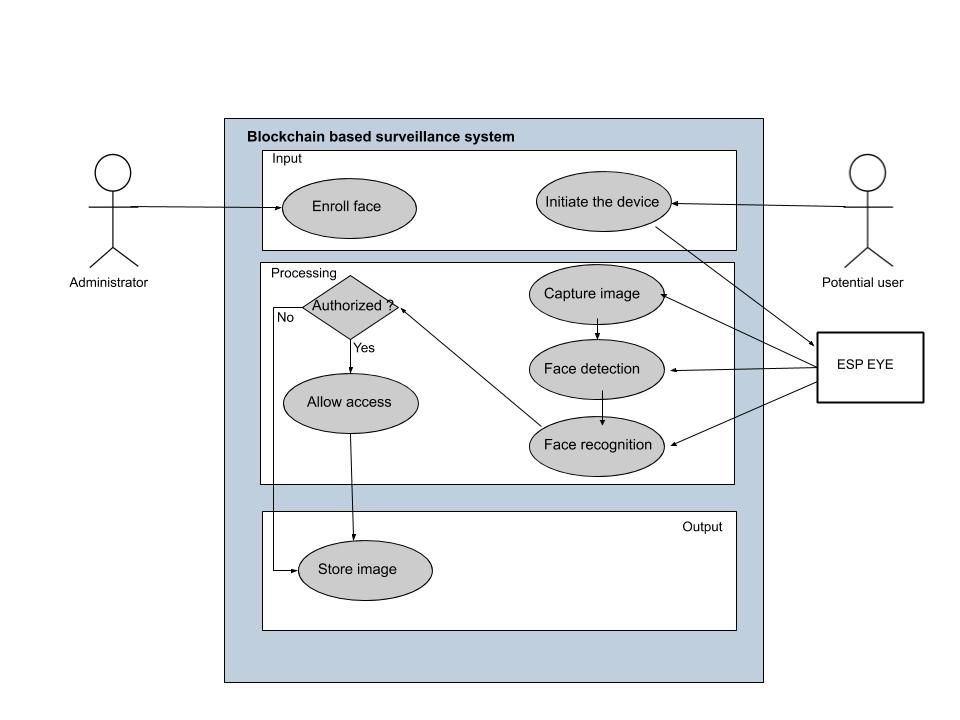
\includegraphics[width=1\textwidth]{figures/use_case.jpg}
    \caption{High Level Overview}
    \label{fig:use_case}
\end{figure}


The assumptions is that the authorized users or individuals are first registered with the system. If an individual is not registered with the system then access is revoked. The process involves an individual approaching an entry point of an institution or a room, where the ESP eye device will detect and recognize the person and grant or reject access. In the due time the ESP WHO platform captures images of individuals and forwards them to the blockchain where it will be stored. Also the cases are considered when a person appears for a continued presence in front of the device. The system shall warn the administrators in such cases. In case of disobedience the system may raise an alarm. 






\section{Thesis Outline}
The rest of the thesis is enumerated in the following order: The second chapter will give a high level approach of the architecture, the hardware used and the design choices that match with the use case which will be compared against other technologies and protocols.

In Chapter ~\ref{chap:lora_and_lorawan} we will introduce and discuss the face detection and recognition algorithms using MTMN which refers to MTCNN (Multi-task Cascaded Convolutional Neural Networks ) and MN (Mobile Nets) for face detection and HFRM (Human Face Recognition Model ) for face recognition. The input for the face detection MTMN is an image captured by the ESP EYE camera and the output is the aligned face which will be as an input for FRMN for face recognition. 

With Hyperledger Fabric we are going add security with the decentralised system by storing all the images of detected individuals. Therefore in order to see the implementation details, its components and the advantages we have allocated Chapter 4 for this. 

In the following chapter, we will dig deeper in the implementation by showing the details of all involved components, the interactions between the components and analyzing the whole architecture. 


In the second-last chapter discusses the future work and improvements of the proposed architecture. Besides  it also lists some limitations that were either coming from the use case or from the technologies. 

Finally, the last chapter encapsulates the whole work by writing the last remarks.

In chapter~\ref{chap:cran_in_cellular}

Chapter~\ref{chap:lora_tools} 



\chapter{Related Work}
\label{chap:related_work}

In this section we are going to provide and introduce the most recent projects and research that shed light on the integration of the three domains. However we are not going to only look on similar architecture but also we will see some similar use cases of real time face detection and recognition for access control. Convergence of the three domains is not by chance therefore in this section we will also list the ideas and benefits that bring the three domains together. 
The ESP EYE development board  provides the basis and the motivation to put more effort on this project. It supports image transmission via Wi-Fi and debugging through a Micro-USB port. 

\section{Synergy of the trio: IoT, AI and Blockchain }

In order to give a better understanding of IoT, AI and blockchain, it mirrors to think of them as an interconnected biological process. IoT is like our brain, which senses billions of connected devices in our planet while producing a universe of new data. AI being the rationale part of the brain. It will be thinking while analyzing data and make a decision based on that. On the other hand blockchain makes me think of memory which stores information in the growing list of blocks.
\subsection{An overview of IoT}

IoT is transforming the world of things around us into a world of sensors that speak about the things. Practically almost anything can be equipped with a sensor and make the things smart. In terms of IoT the sensors are not just used to detect and measure but they are also to respond to changes thanks to the proliferation of internet-enabled devices which are embedded with computational power. 

The number of IoT devices took over the population worldwide since 2008. Based on (ref123) the number of IoT devices is expected to increase and reach around 31 billion by the end of 2020. However this number is not expected to ever stop but it will be double by the end of 2025 as depicted in Figure~\ref{fig:num_of_iot} (ref124).

Most IoT devices run on microcontrollers or microprocessors with very minimal processing power which makes them less powered than a smartphone. The reason behind is not that such devices cannot be equipped with more processing power but to be energy efficient and run with mimimal power on battery and reducing environmental impacts of the energy use. With such growing number of IoT devices in the near future it will eventually pose a challenge even without increasing the processing power of such devices. Eventualy there will be a high demand of developing a green communication accross the network (ref126). This will at some point also affect the developers IoT devices who will have to find more lightweight programs to run high consuming energy programs such as deep learning. As a result different algorithmic approaches are taking place and more efficient algorithms are being developed (ref128).






\begin{figure}[!htb]
    \centering
    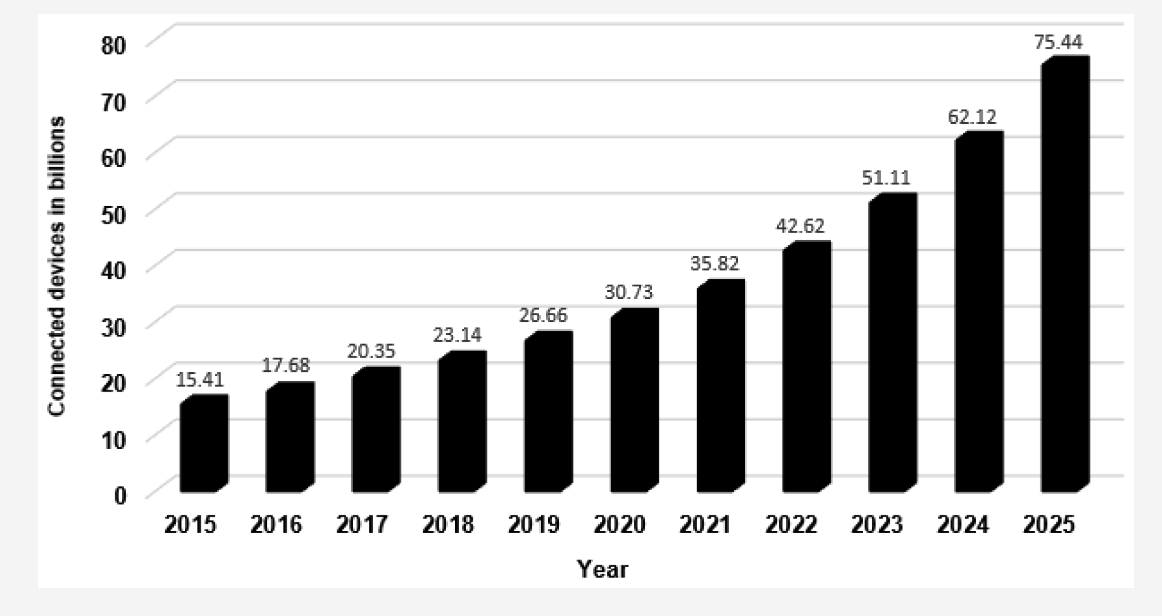
\includegraphics[width=1\textwidth]{figures/number_of_iot.png}
    \caption{The growth of IoT devices from 2015 to 2025 ref(img1)}
    \label{fig:num_of_iot}
\end{figure}


We would like to mention a number of common characteristics that most IoT devices share: 

\begin{itemize}
    \item Connectivity - with the help of a number of protocols they can communicat with each other.
    \item Heterogeneity: a variety of devices and objects including communication protocols
    \item Unique identity: a unique identifier for each device 
    \item Big data: IoT number one source of big data 
\end{itemize}

However IoT suffers from its typical architecture design which is the centralized architecture. These centralized server either on the cloud or on premise manages and deals with all requests coming from various nodes. This architecture comes with multiple challenges: scalability issues, security and privacy challenges and issues with the analysis of big data (ref130). 

\subsection{Enabling Deep Learning in IoT}
AI has become a buzzword and one of the topics that has a significant impact on many different domains. In Figure~\ref{fig:ai_terms} depicts the relationship between Artificial Intelligence, Machine Learning and Deep Learning. In simple words AI encapsulates the imitation of human intelligence by computers. Machine learning is the technique used to allow computer programs to access data and use it to automatically learn and improve from experience. The neural network involves a large number of processors operating in parallel arranged in tiers , in the same way neurons in our brain works. While deep learning employees neural networks but with many layers of neural networks. 


\begin{figure}[!htb]
    \centering
    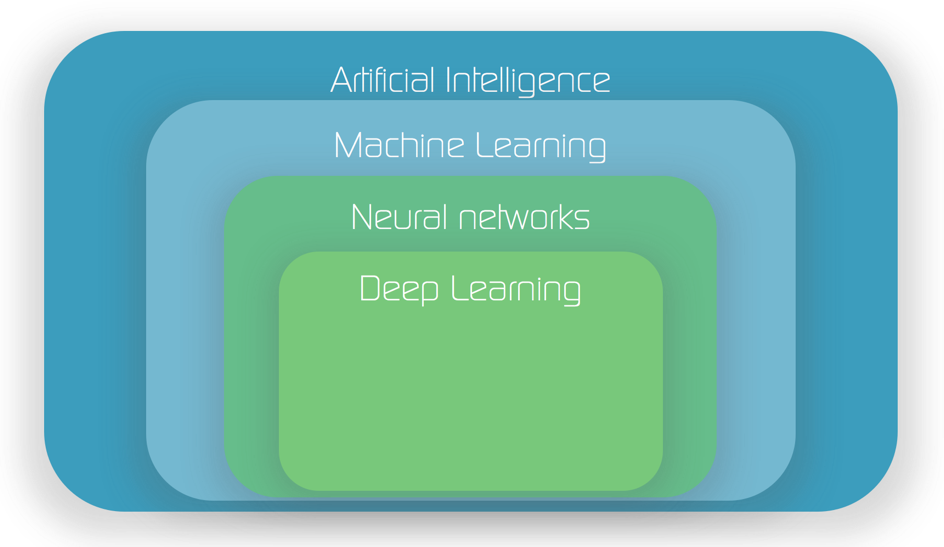
\includegraphics[width=1\textwidth]{figures/ai_classification.png}
    \caption{Relationship of AI terms.(refimg12)}
    \label{fig:ai_terms}
\end{figure}
We already know that AI can solve and make sense of the immense amount of data produced from IoT devices. However the main question for research appears “How to deploy neural networks directly on these tiny devices? Therefore there is an opportunity and challenge at the same time to run machine learning on such tiny IoT devices based on microcontrollers. By running machine learning on these tiny devices, we can directly perform real time data analytics in the device itself, therefore avoiding the need to store all the data generated from the IoT device. Typically commercial use cases of smart IoT devices often offload the Artificial Intelligence part to the cloud. 
One of the most recent study(ref321) that worked on this direction tested two approaches with deep learning: 
\begin{itemize}
    \item Offloading deep learning platforms to the cloud
    \item Migrate deep learning to an IoT device
\end{itemize}

The two approaches were tested and look from two different perspectives,  whether offloading machine learning can reduce energy efficiency and satisfy the real time requirements of object recognition. 
In the first approach they used convolutional neural networks on the cloud, while the Jetson TX1 was responsible to just take images and forward them to the cloud. The results show that executing machine learning in the Jetson TX1 consumed more energy compared to the offloading to the cloud. However offloading AI to the cloud also comes with drawbacks, it has lead to a range of latency starting from 2 seconds that goes up to 5 seconds which is far higher compare to the execution of AI in the Jetson TX1 itself. This leads to conclude that the variability of response time make it quite unreliable and not useful for real time AI processing. 

Furthermore MIT researchers ref(mit123) have implemented a sytem called MCUNet, which has a high potential to bring deep learning in much smaller devices like tiny computer chips despite their limited memory and computational power. 

\subsection{Intersection of Blockchain and AI}

There is a high research on Blockchain and AI but analysed in isolation and in various domains and applications. Some research ref(17) focus on the application of AI in the Blockchain for making blockchain more efficient for instance, consensus mechanisms and better governance. However there seem to be more research and applications of Blockchain in AI. Similar to IoT, AI domain also suffers from security, its centralized architecture and resource limitations. This is exactly what blockchain is looking to solve. There is a lot of discussion and research in this area, however most of them are reviews and solutions that do not provide a use case or implement such solutions. In order to have a global image the Table ref() describes the features of the two technologies and the benefits of integrating such features.

There is another interesting contribution (ref) that came up with an AI blockchain platform to fight the propagation of fake news. This platform allows publishers to setup a distribution platform in the blockchain while AI will be monitoring on the actors who are adding news to the blockchain. Expectation is that the blockchain will server as the "factual database" to trace back the news. So the news which cannot be traced back to the blockchain will be automatically considered fake. 




\begin{table}[hbt!]

    
    \begin{tabular}{  p{4.4cm}  p{4.4cm}  p{5.4cm} }
      
\textbf{Blockchain}      
& \textbf{AI}   
& \textbf{Benefits of blockchain} \\\midrule
Decentralized & Centralized        
& Enhanced Data Security \\\hline

Immutable & Probabilistic       
& Collective Decision making \\\hline


Data Integrity & Volatile      
& Decentralized Intelligence \\\hline

Resilient to attacks & Data, knowledge and decision centric     
& High Efficiency \\\hline

Deterministic  &
Changing      
& Improved trust on robotics decision \\
        \bottomrule
    \end{tabular}
    \caption{Benefits of integrating blockchain into AI  (adopted from \ldots%\citealt{crouch2012doing}
    )}
    \label{crouch}
\end{table}

\subsection{Integration of Blockchain with IoT}

We have already listed a number of issues that IoT world is facing, which mainly is the centraized architecture, security and privacy. Therefore pretty much of the research is focused in this area, typically with the advantages of blockchain those gaps can be closed. For instance ref(IS) attempted to discover the security gaps that could be mitigated with the help of the blockchain to ensure the reliability and availability of the data.

Other studies (refIS) attempted to integrate crypto based blockchains such as Ethereum in their approaches. We argue here that most of the crypto based blockchains are not efficient in storing data coming from IoT devices. First users have to pay fees for each transactions and the there is a limitation in the number of transactions it can process. Although we can escape from the centralization still there is the risk of bottleneck. Therefore in our study we will be using Hyperledger Fabric a non crypto based blockchain aimed for storing data. 


































\begin{comment}

\begin{table}[!h]
\definecolor{LightCyan}{rgb}{0.88,1,1}
\definecolor{Gray}{gray}{0.9}
\newcolumntype{g}{>{\columncolor{LightCyan}}c}
\noindent\begin{tabularx}{\textwidth}{|g|l|X|}

\hline apple  & StackOverflow & Dardh \\
\hline 
\begin{itemize}
\item[--] Decentralized

\item[--] Deterministic
\item[--] Immutable
\item[--] Data Integrity

\end{itemize}

& StackOverflow &
 lots of long text. lots of long text. lots of long text. lots of long text. lots of long text. \\
\hline 

\end{tabularx}
\caption{Truth Tables and Accuracy Measures for each modeling library.}
    \label{tab:truthTables}

 \end{table}



\end{comment}

 
 
 
 \section{Use cases on AI, IoT and Blockchain}
 
 We have already described the intersections on how Blockchain, AI and IoT accommodate each other in pair, however there is a very high potential for the usage of all the three domains in one use case. With such a high number of IoT devices there is a potential to take the advantage of AI and Blockchain at the same time. Based on reforacle, every institution  which will take the advantage of exploiting these technologies, it will have the chance to radically enhance their existing processes and create entirely new business models. 
 
An interesting work ref(smartcity)  presents how the collaboration of the three domains can build a sustainable smart city. Given the many issues people in urban areas face, the concept of the sustainable smart city brings new opportunities for the application. With their new approach they aim to have a transparent monitoring system for measuring pollution which in turn will help raise awareness to the population. 

In another use case the authors (refhomeauto) propose an IoT based home automation and surveillance system. In this setup they have employed a raspberry pi, a camera attached to it and a DC motor for controlling the door. The video surveillance is not detecting or recognizing people, so the burden falls into the owner who through the help of a front end will be able to open the door. Therefore compare to our solution there is no AI and blockchain integrated. 


A use case that pretty much is matching with our use case is a design and implementation of a camera based sensor for room capacity monitoring. The aim of it is to count the number of people present in a room with the help of a raspberry pi and a camera. In Figure~\ref{fig:raum} we can see the architectural overview. 

\begin{figure}[!htb]
    \centering
    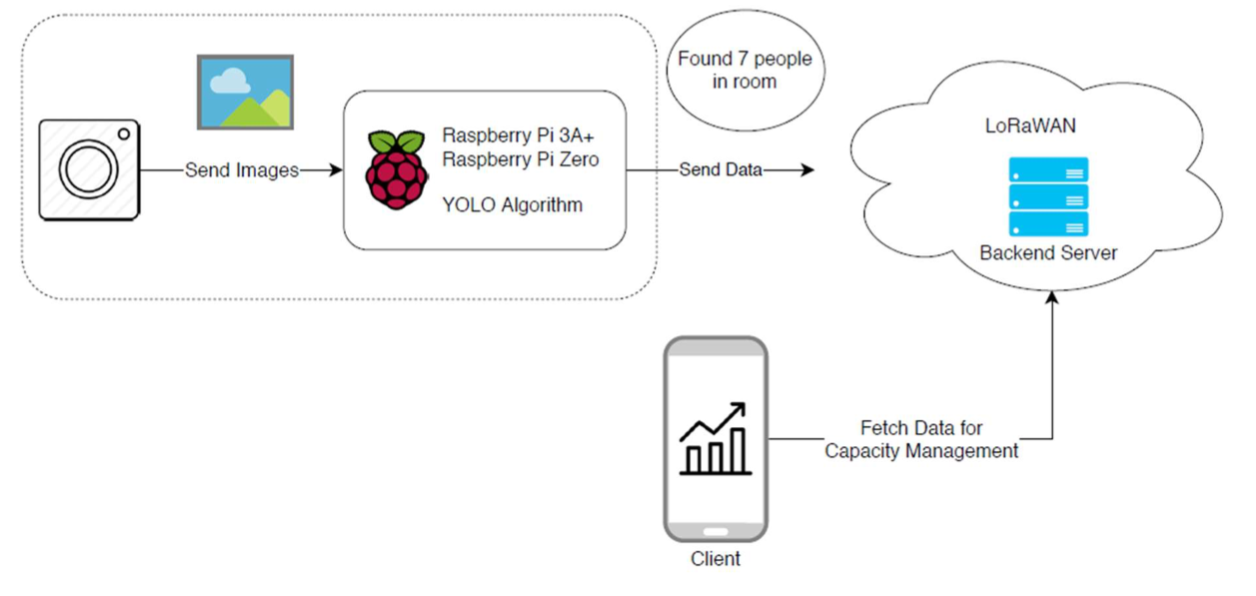
\includegraphics[width=1\textwidth]{figures/raumbelegung.png}
    \caption{Architectural Overview(ref)}
    \label{fig:raum}
\end{figure}

Their architecture employees AI and IoT. This use case was designed and implemented by a group of students at FHNWS who employed a raspberry pi equipped with camera and lora gateway. The role of camera is to just take pictures and after that some machine learning algorithm will analyze the image and find the number of people in the room. Once done the data is then send to a LoraWan Server. To achieve that they have attached a LoraWan antenna to the RPI and eventually with a front end they can monitor the room. So face detection happens in the RPI, the algorithm counts the number of people in the image and sends it to the Lorawan Backend Server. From here we can conclude that the issue of centralisation is still open, data is being stored in a database, security issues are not tackled enough. Besides there is also the need for a RPI to be placed in a room as the camera is attached to it and that needs power to run. 

With out proposed architecture we are not only going automate the IoT-based surveillance system but provide a robust solution that will take care of the leaks that AI and blockchain will be able to neutralize. 


\chapter{Face Detection and Recognition in Esp Eye}
\label{chap:face_detection}
\section{Background of real time face recognition in low powered IoT devices}
Monitoring and tracking people and their activities with the current approaches of the surveillance system normally generate enormous amount of data coming from Internet of Things devices. This leads to a number of issues that need to be treated well, data migration from camera over a limited bandwidth for face detection and recognition leads to high latency  and the camera positions need to be placed near the electrical plug as they require a lot of power. Therefore this approach leads to generating a lot of data while transferring it to a different source for face detection and recognition. Besides many public places use surveillance camera for video capture based on motion detection, which means that once someone approaches near the camera it will start recording and throughout the day you can imagine how much volume of data can be generated. 
In this chapter we will guide you through the existing algorithms for face detection and recognition and then we will see the algorithms that are implemented for the resource constraint devices or IoT. Therefore we will also discuss the reason behind choosing to deploy the face detection and recognition algorithm in the ESP EYE itself. In addition the Multi-task Cascaded Convolutional Networks (MTCNN) and  Human Face Recognition Model (FRMN) for face detection and recognition will be described in detail. 


\subsection{The generic framework for face detection and recognition}


Face detection is normally the first step towards face recognition or verification as it can be seen in  Figure~\ref{fig:framework}. Basically the framework follows a two step process: face image detecting and face recognizer. In the first process an image is taken from the camera which searches for human faces in that image then the algorithm localizes the face from the background image. This process happens continuously which means if there is no face detected then it captures the next image and does the same. When no face is detected the image is deleted from memory. The next process assumes the image is taken and a face has been detected then the face recognition will start. In this phase another algorithm will take place in order to determine who are the persons in that image. During both processes, algorithms extract features or a pattern which is the key step of the algorithm. Feature extraction is the process is essential for localizing facial components such as mouth, nose, eye and others. 

\begin{figure}[!htb]
    \centering
    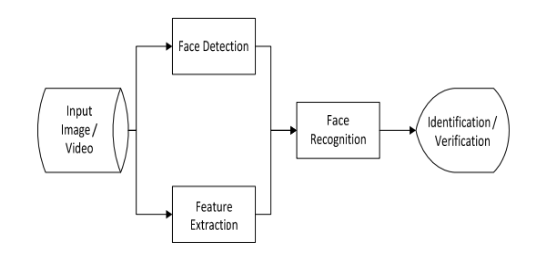
\includegraphics[width=1\textwidth]{figures/framework.jpg}
    \caption{ Face detection and recognition.}
    \label{fig:framework}
\end{figure}


\subsection{Existing  algorithms  for  face detection and recognition}

There are a number of algorithms that have been developed and now used to tackle the face detection and recognition issues. We would like to mention a number of successful algorithms which are widely used and they are: 

\begin{itemize}
    \item \textbf{Principle Component Analysis (PCA).} It is a statistical approach and one of the simplest in face recognition systems. In this approach images with detected faces are transformed into eigenfaces. Eigenface is a method that determines the variance of faces from a collection of images. The main idea behind is to linearly project images onto a lower dimensional images. 
    
    
    \item \textbf{Linear Discriminant Analysis (LDA).}
   It is a method used in pattern recognition and machine learning by finding a linear combination of features. It used for dimensionality reduction and performs very well in face recognition. It finds a projection transformation by maximizing the between-class distance and minimizing the within-class distance. 
   
   
   
    \item \textbf{Skin colour based algorithm.}
    As the name says, it uses skin color as a feature for face detection and it is fast, self adaptive algorithm. From the input image it uses color space for the skin region. A bounding box is drawn to extract the face from the image.
    
    
    \item \textbf{Wavelet based algorithm}
    In this method the image is cut up into a subset of frequency components and to each component is applied a mathematical function. One of the widely known algorithm is the Gabor wavelet.
    \item \textbf{Artificial  neural  networks  based  algorithm}
    Typically face recognition is achieved with the help of deep learning more specifically the Convolutional Neural Network. Through a multy-layered network which performs a specific task using classification.
\end{itemize}


\subsection{Hardware requirements for running real time face recognition}

It is important to mention that a typical computer or a laptop possess an AMD processor, while a raspberry pi and smart phones and some other devices like watches are equipped with a ARM processor. Obviously ARM architecture offers lower performance compare to AMD, but there is a reason behind, the ARM processors consume less power than AMD processors. Performing real time recognition on both AMD and ARM is not an issue, both can handle them. However both processors need power either plugged or if on battery they can last max one day long. In contrast the low powered IoT devices can run for years with a typical voltage of 3.6 V. Therefore to our knowledge so far it is not possible to perform real time recognition with a processor other then the above mentioned, AMD and ARM. 

ESP EYE is the first device to perform real time face recognition. However, this does not mean that the face detection and recognition algorithm have been used one to one. ESP EYE is one of its kind that comes with ESP WHO platform which supports both face detection and face recognition. The ESP EYE is equipped with Tensilica LX6 dual core processor. To our knowledge this is the only device that can perform real time face recognition in a microprocessor that lies out of the two classes AMD and ARM processors. 

\section{Face detection with deep learning using Multi-Technology Network Management (MTNN)}

MTMN refers to both MTCNN (Multi-task Cascaded Convolutional Networks) and MobileNets. There are a number of deep learning methods that have been implemented and paved the way for face detection but MTCNN is a framework which integrates both face detection and alignment. With the help of MobileNets it builds light weight deep neural networks which uses depth-wise separable convolutions for face detection.


\subsection{MTCNN a three layer CNN model}

MTCNN is one of the state of the art approaches which is described and published in the paper "Joint Face Detection and Alignment Using Multitask Cascaded Convolutional Networks" ref(mtcnn) in 2016. MTCNN is popular because it has achieved 95 percent accuracy on a range of banchmark datasets. MTCNN is a novel approach because it performs a lightweight Convolutional Neural Network based framework which actually performs simultaneously face detection and alignment whereas in other CNN-based frameworks face detection and alignment are two distinct processes.   
Due to its lightweight CNN architecture it can perform in real time which is possible to run it in an ESP32 chip. 

The process consists of three stages of Convolutional Neural Networks that are able to detect faces and landmark location such as eyes, nose, and mouth : 

\begin{itemize}
    \item \textbf{P-net} 
    \item \textbf{R-net} 
    \item \textbf{O-net} 
\end{itemize}


The Figure~\ref{fig:mtcnn} adapted from the paper depicts a summary of the three layers with the output of each layers on the right side. The three mentioned models perform independent of each other, the output of each is used as an input of another. 
First of all once the image is captured it will be scaled into multiple different sizes based on different scaling ratios which forms a collection of images called Image Pyramid similarly as in Figure~\ref{fig:pyramid}. This will allow the model to learn different image scales effectively. This type of image processing is used extensively because it makes it easier to detect faces no matter how far or close they stand in the image.


\begin{figure}[!htb]
    \centering
    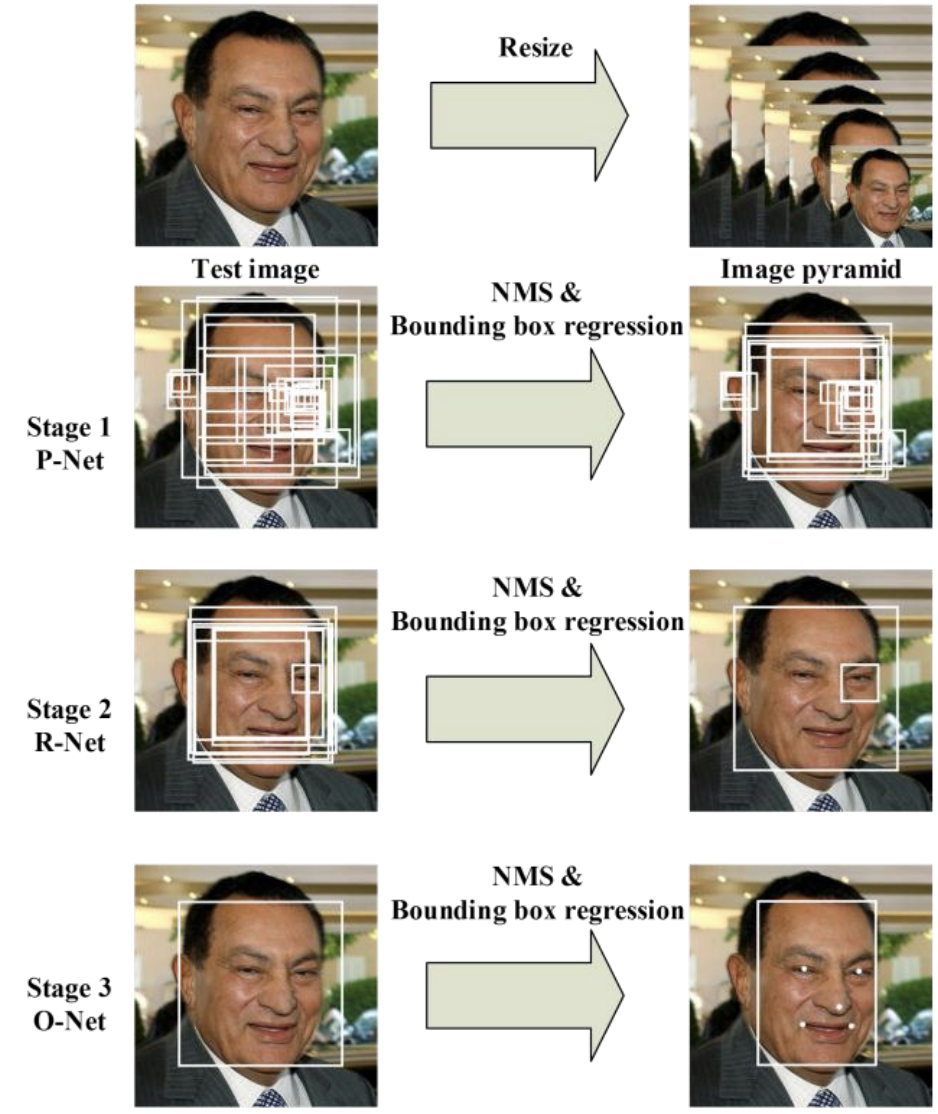
\includegraphics[width=1\textwidth]{figures/mtcnn.png}
    \caption{ Pipeline of MTCNN that includes three-stage multi-task deep convolutional networks.}
    \label{fig:mtcnn}
\end{figure}

\begin{figure}[!htb]
    \centering
    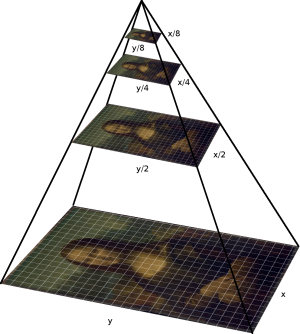
\includegraphics[width=1\textwidth]{figures/pyramid.png}
    \caption{ Image rescaled in a form of a pyramid}
    \label{fig:pyramid}
\end{figure}

\subsubsection{Proposal Network or P-net}

The first stage of Proposal network (P-Net) as depicted in Figure~\ref{fig:3stages} is a full convolutional neural network which extracts face candidate regions from images at various scales and bounding box regression vectors. Bounding-box regression is a technique for refining or localizing boxes in objects. In other words it is a rectangle which is drawn over the image to emphasize the face. For each of the scaled image that reside in the image pyramid it runs a 12x12 kernel which starts in the top left corner or at these coordinates (0,0) to (12,12). This portion of the image 12x12x3 will be the input for P-Net as it can be seen in Figure~\ref{fig:3stages}. To this image then is run another kernel of size 3x3 and then it produces feature map or smaller images depending on the stride. For example in the first filtering it produces feature maps of size 5x5. The stride is the number of jumps or pixels that the kernel moves to apply a filter. In order to deliver a 5x5x10 from 12x12x3 with a kernel 3x3 the stride is 2. Therefore stride plays a role in time complexity of the algorithm, the lower the stride the higher the time complexity. From this 12x12 portion of a scaled image from pyramid the P-net will output the coordinates of a bounding box if there is a face. Before releasing the last output bounding box coordinates a number of similar boxes are filtered out with lower confidence and only the ones with higher confidence are kept. The bounding boxes left may still overlap as in Figure~\ref{fig:non-max}, therefore we need the one that perfectly covers the face. To do that the non-max suppression technique is applied which reduces the number of boxes by taking the best fit and not the one the network is more confident in. 




The aim of the this network is to check whether there is a face in the input and output the face frame or box with the four coordinates. In the face classification the network outputs the probability of being a face and not being a face and both values add up to 1. The bounding box holds the exact position of the box with coordinates. 


\begin{figure}[!htb]
    \centering
    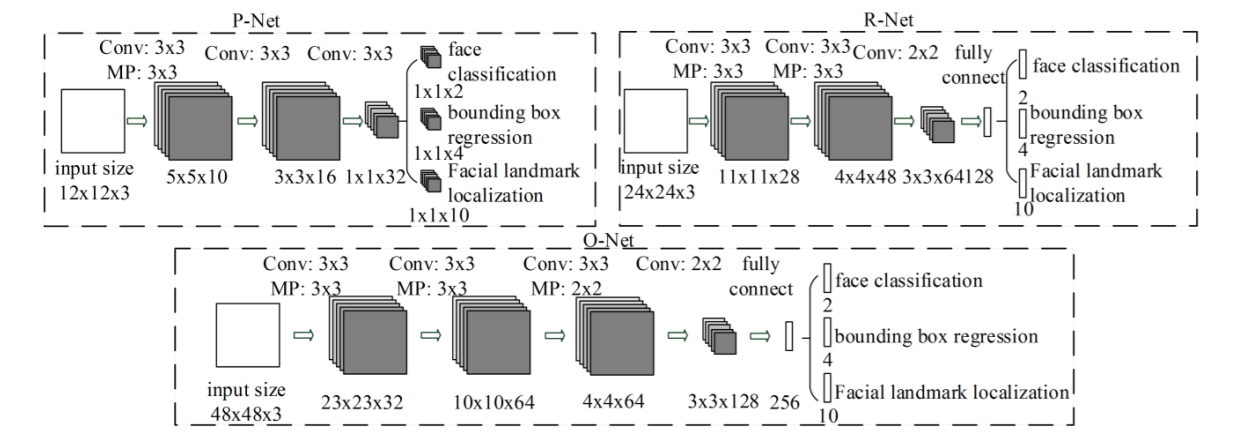
\includegraphics[width=1\textwidth]{figures/3stages.png}
    \caption{ MTCCN: P-Net, R-Net and O-Net structure}
    \label{fig:3stages}
\end{figure}


\begin{figure}[!htb]
    \centering
    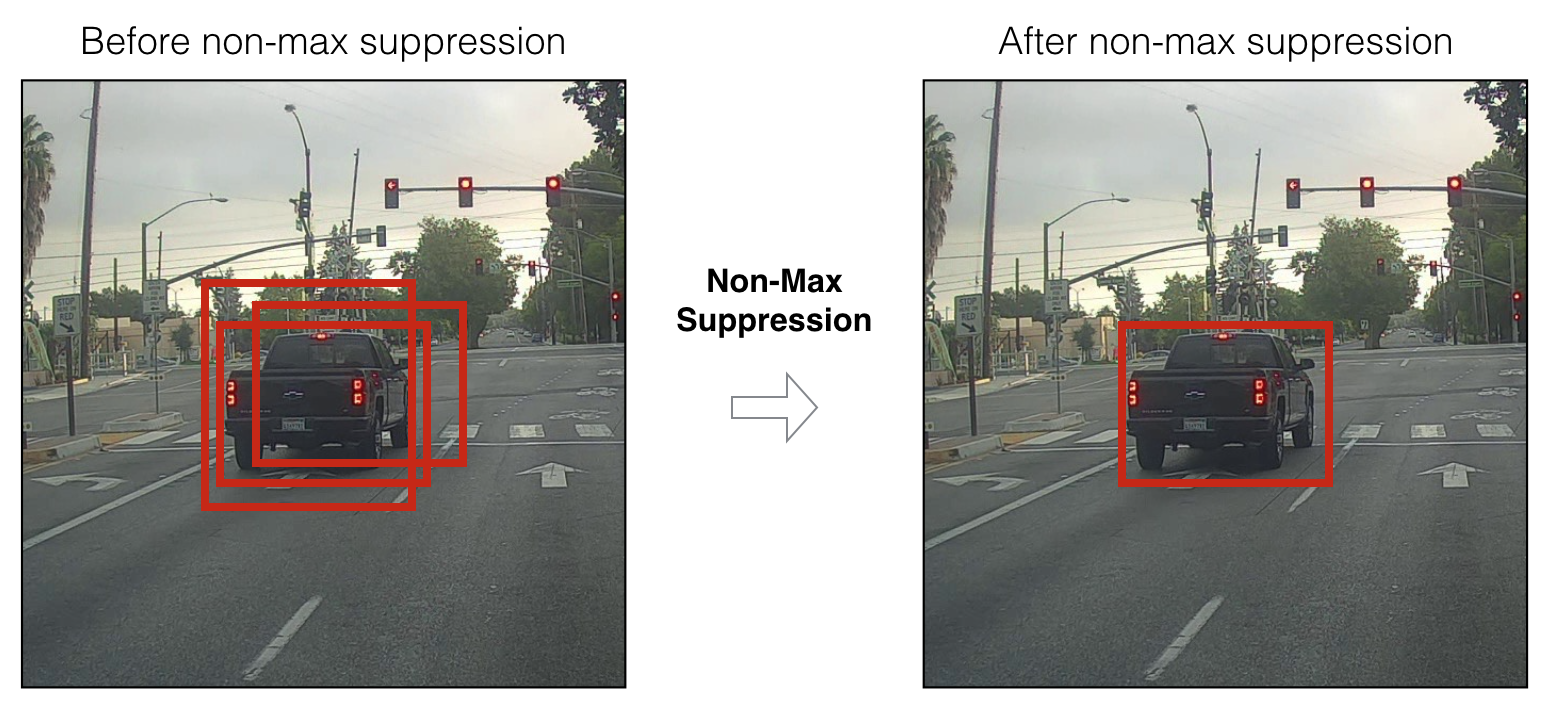
\includegraphics[width=1\textwidth]{figures/non-max.png}
    \caption{ Non-Maximum Suppression}
    \label{fig:non-max}
\end{figure}
\subsubsection{Refine Network or R-net}

The structure of R-net can be seen in the Figure~\ref{fig:3stages} which looks pretty much the same as R-net. R-net is a rough prediction of faces therefore there are a number of false positives so the aim of R-net is refinement of the bounding boxes and reduce the number of false positives.
The input of this stage is the bounding box generated by P-net which can be of different sizes. From the Figure~\ref{fig:3stages} we can see that the input size is of size 24x24x3. So regardless of the size of the bounding box it still needs to be scaled to the expected input size before sending to R-Net. Therefore the bounding boxes will be scaled to 24 x 24 pixels and now we can feed them to R-Net. Once again the same as in P-net happens, get rid of boxes with low confidence and apply the NMS on every survived box. The output is the same as of that of P-net which also consists of the tree parts: probability of being a face or not, square frames and the position of the landmarks. This stage can help to recover the weaknesses of P-net and improve accuracy by reducing the number of false positives. 


\subsubsection{Output Network or O-Net}

In the Output Network almost the same happens as in R-Net with some changes in middle layer where additional channels are added which means accuracy is also increasing. The input, feature maps are getting higher and higher in terms of pixels. The accuracy rate is expected to be higher which is proportional to the increased time complexity. In this case the output of R-Net will be the input but scaled to 48x48x3. 
Now we can already see the reason behind using three neural networks and not one. Since the final decision is received from O-Net we can directly use it and avoid the previous two networks. But the speed will be very slow since O-Net will have to do a lot of operation on all candidate windows which can be very high. With the help of P-net and R-Net a lot of non relevant windows will be filtered out from the start. From P-Net to R-Net a lot filtering happens, so the advantage here is to perform fine grained face detection only on highly probable candidate windows. To make the story short here is a summary of the whole face detection process: 
 
 P-Net:
\begin{enumerate}
  \vspace{-0.7cm} \item Image is captured by ESP EYE.
  \vspace{-0.3cm}\item Create image pyramid with multiple scaled copies of the image.
  \vspace{-0.3cm} \item Pass each image of pyramid to P-net.
  \vspace{-0.3cm} \item Candidate windows as output.
  \vspace{-0.3cm} \item Filter out bounding boxes with low confidence.
  \vspace{-0.3cm} \item Adjust the current 12 x 12 kernel coordinates to “un-scaled image” from pyramid.
  \vspace{-0.3cm} \item Non-Maximum Suppression for all kernels.
   \vspace{-0.3cm} \item Adjust the bounding box coordinates to “un-scaled image”.
   \vspace{-0.3cm} \item Candidate windows as output.
\end{enumerate}

 R-Net:
\begin{enumerate}
  \vspace{-0.7cm} \item Pass the bounding boxes
   \vspace{-0.3cm} \item Pass each image of pyramid to P-net.
  \vspace{-0.3cm} \item Candidate windows as output.
  \vspace{-0.3cm} \item Repeat step 5 to 9 of P-net.
\end{enumerate}


 O-Net: Repeat the same steps as in R-Net

\subsection{MobileNetsv2 for lightweight CNN}

MobileNet is a CNN architecture developed by researchers at Google which typically is used for in Image Classification and Mobile vision. The model is proven to build light-weight deep neural networks which uses less computational power to run. This architecture allows to run face detection and recognition for IoT devices, Mobile devices and computers with low computational efficiency without compromising the accuracy of the results. MobilNet version 2 is the recent version which comes with a research paper published in late 2018. It is a refinement of the MobileNet version 1 which make it even more powerful. 

In order to understand why this model is being used and at which step in face detection is used we would like to first give a quick recall on how convolutional neural network works. CNN is composed of neural networks as in Figure~\ref{fig:3stages} which in our case receives an image  and transform it through a series of hidden layers. Each hidden layer is made up of a number of neurons which are nothing else but mathematical functions and in terminology it is called activation function which calculates the weighted sum of multiple pixels and decides whether or not to send a signal to the next neuron. The activation function takes the weighted sum of all inputs plus the bias.

Before reaching the next neuron, a convolution or a filter is applied to the input image and a feature map is created from it. We can see in P-net in the first layer there are 10 feature maps created with a size of 5x5. That means a convolutional filter is applied 10 times to the input image, the size of the kernel in our case is 3x3. But this does not mean that the same filter is applied but different ones as in Figure~\ref{fig:filter}. This kernel slides accross all the pixels of the input image by covering all of them and at each step it computes the weighted sum and puts in the feature map or a in the newly generated image as in Figure~\ref{fig:conv}. Depending on the size of the kernel and input image the new image normally the new feature map will have a smaller size. Here is where pooling comes into play, with pooling we can upsample or downsample or change the spatial dimensions but in fact only max-pooling is performed because there we need to find outliers which is the moment the network can detect features. So the deeper we go in the image the better to detect features. When the output of the P-net was generated which is an image or candidate window it had to be upsampled because R-Net only receives image of dimensions 24x24x3. This means we are somehow zooming in the image more and more until the last network is performed. Besides we can also see that the number of filters is increasing and in the last layer of O-Net we can see feature map of dimensions 3x3x128 which means 128 filters have been applied. 
\begin{figure}[!htb]
    \centering
    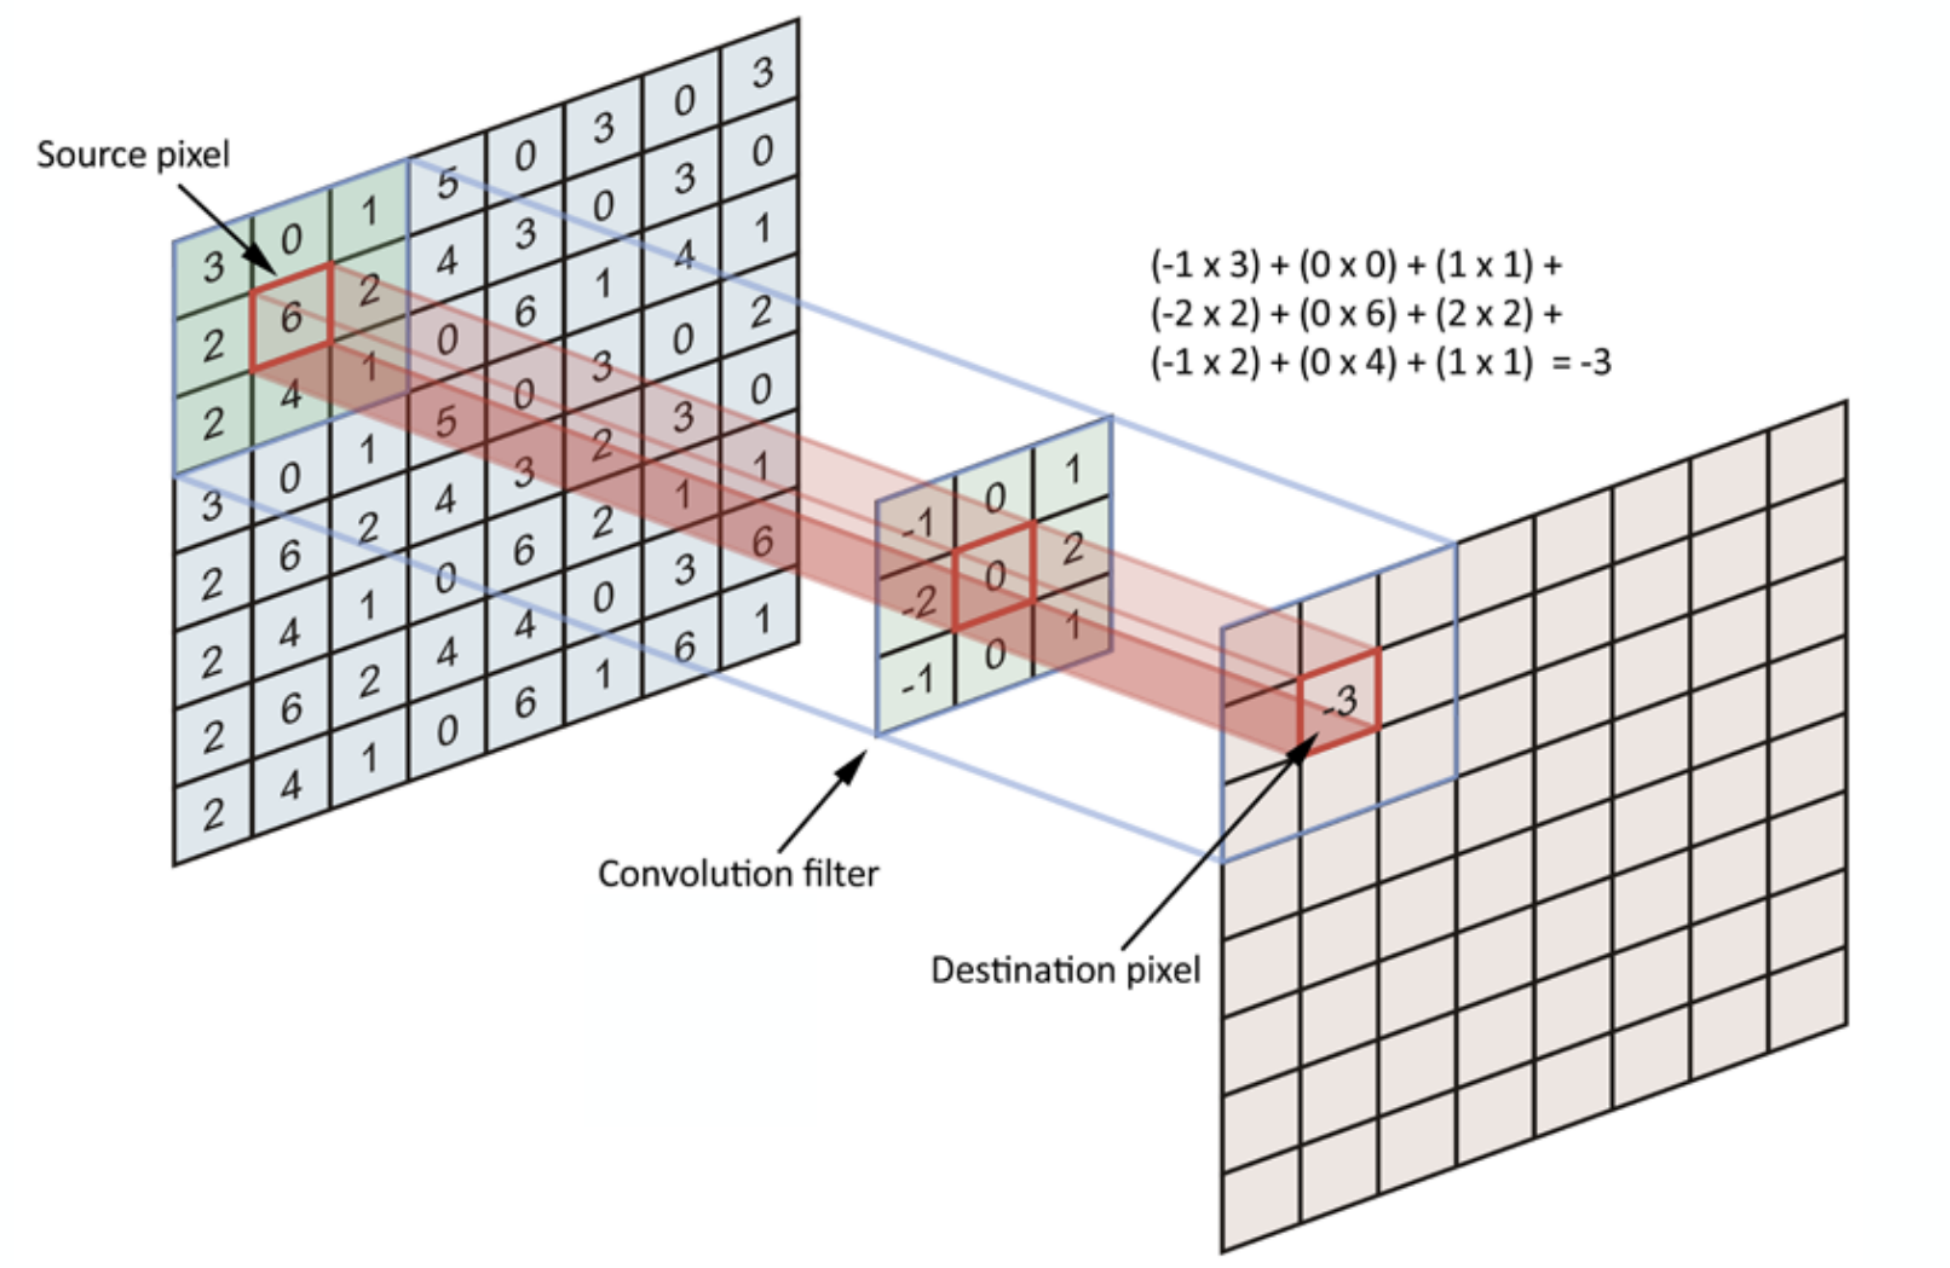
\includegraphics[width=1\textwidth]{figures/convolution.png}
    \caption{The convolution operation}
    \label{fig:conv}
\end{figure}


\begin{figure}[!htb]
    \centering
    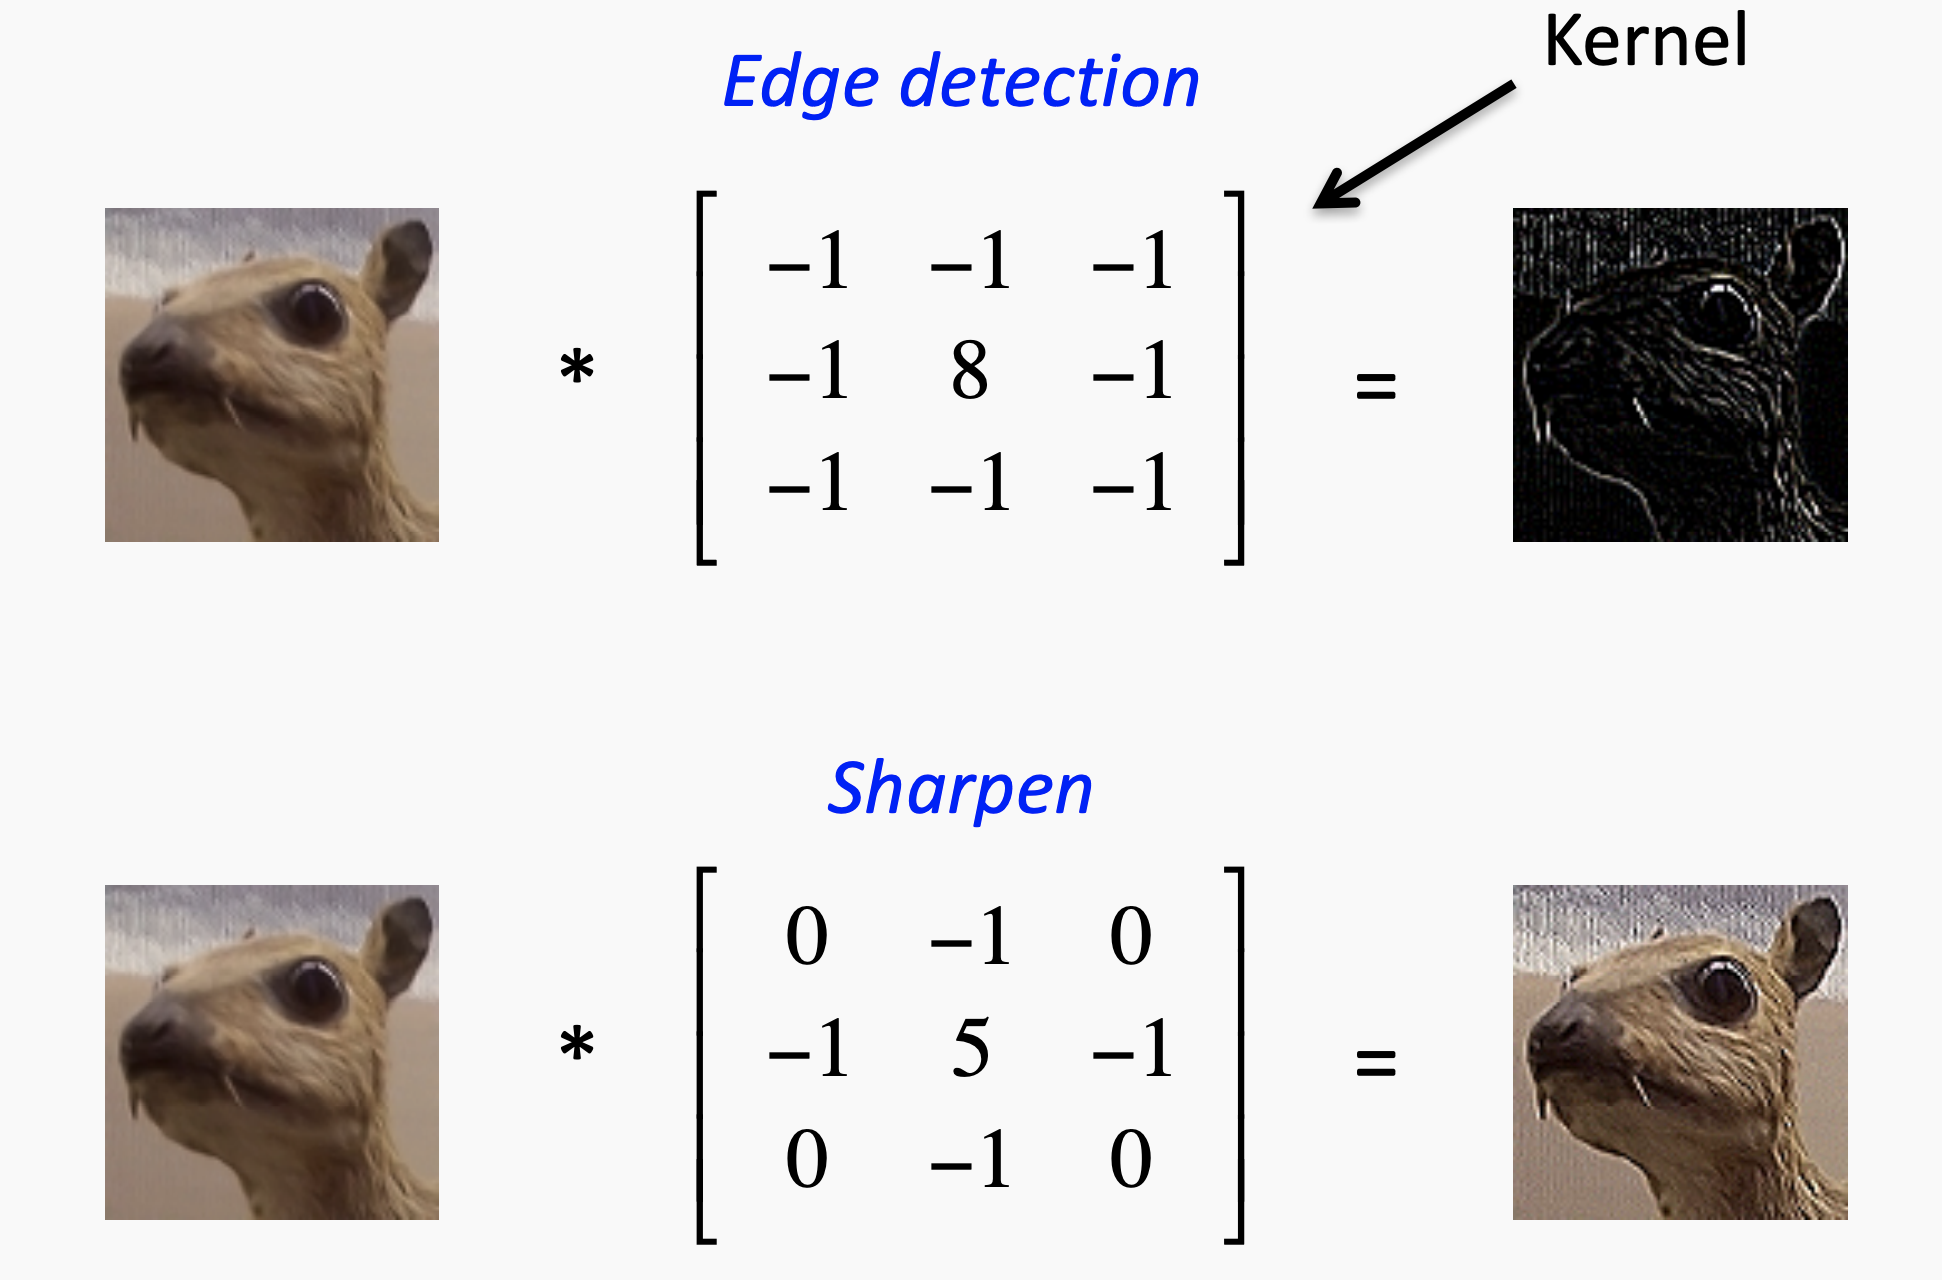
\includegraphics[width=1\textwidth]{figures/filters.png}
    \caption{Examples of filters}
    \label{fig:filter}
\end{figure}
From here we can understand the reason behind the staging. Performing the convolution to the image directly from the last stage we would need a lot of computation because filtering obviously takes time. Imagine having an image where the person to be detected is standing far away and in the image that person may cover for example only 5x5 pixels out of an image of 360x240. So applying a high number of filters in each extracted image with 5x5 pixels is not efficient. So the idea is to first apply filtering in larger parts of the image so that we can get rid of candidate windows which do not include faces.

The staging approach is quite efficient in face detection while MobileNets is essential in the way convolution is performed in applying the filters and creating feature maps. 



\subsubsection{Normal Convolution}

The main idea behind MobileNetv2 is to get high accuracy with less computational power. In the regular convolution, the convolution kernel or the filter is applied on all the channels of the input image. The input image will normally have 3 channels and for each color RGB there is one channel. Let's assume we have an image of 12x12x3 pixels as in Figure~\ref{fig:normconv} and we do convolution with kernel of size 5x5 and a stride 1. When applying the kernel it multiplies each pixels with its counterpart and at the end we get a feature map of 8x8x1. No matter how many channels the image has it only writes one pixels with only one channel.
However since there are 3 channels we need to also have the convolutional kernel with 3 channels. So instead of doing 25 computations but we have to do 5x5x3=75 multiplications with quadratic time complexity. And at the end we receive a feature map with one channel. 

\begin{figure}[!htb]
    \centering
    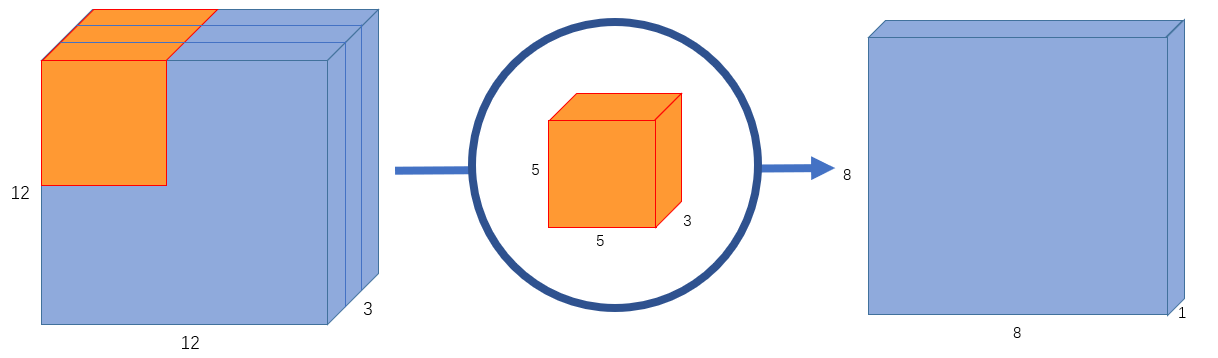
\includegraphics[width=1\textwidth]{figures/normalconvolution2.png}
    \caption{Normal convolution}
    \label{fig:normconv}
\end{figure}

Therefore if we want to have a feature map with more dimensions then we need to apply more kernels. If we want a feature map with 256 channels then we have to apply the 5x5x3 kernel 256 times. Normally this is how convolution works but this is not the case with the MobileNets architecture. MobileNets is using this approach just once at the very first layer. In all other layers it employees the depthwise separable convolution with two parts: depthwise convolution and pointwise convolution. 



\subsubsection{Depthwise convolution}
 

With depthwise convolution instead of applying one kernel with 3 channels we apply 3 kernels with one channel. Here we do not combine the three channels but perform it separately. This makes it easier to create a feature map with multiple channels. With normal convolution to achieve this we have to apply the kernel with 3 channels 3 times, but here the number of kernels stays the same but with linear time complexity. 
The advantage is to filter each input channel separately for edge detecting and so on. 



\begin{figure}[!htb]
    \centering
    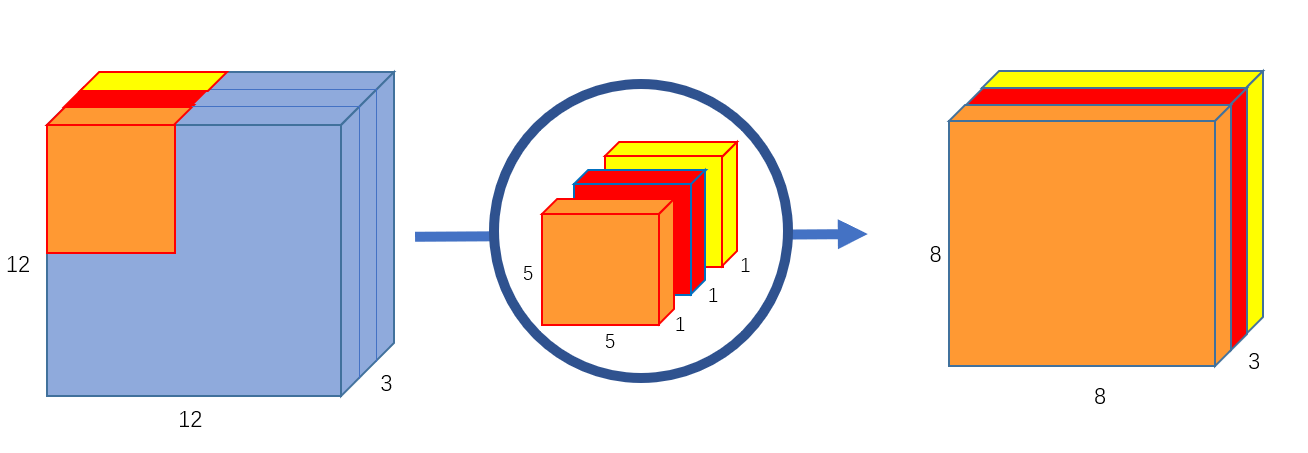
\includegraphics[width=1\textwidth]{figures/depthwise2.png}
    \caption{Depthwise convolution}
    \label{fig:depthconv}
\end{figure}

\subsubsection{Pointwise convolution}
As of now we have transformed the image into 8x8x3
So now if we want to increase the number of channels to 256 as in normal convolution above we apply a pointwise convolution. As the name say pointwise convolution applies a kernel of size 1x1x3. At this step we come back again to normal convolution, so now we apply the kernel to the image 8x8x3 from Figure~\ref{fig:depthconv} and combine it to form a one channel image with output a 8x8x1. To get 256 channels we apply the same kernel 256 times. Now we have the same feature map as in normal convolution above but with less number of computations. 

Here is a simple calculation of the both approaches, normal convolution and MobileNet approach. 
Assuming we have an input image of size 12x12x3 and the kernel is of size 5x5 and stride 1, with these parameters we will get an image of size 8x8.
With normal convolution since the input image has 3 channels we apply the kernel 5x5x3 we get an output image of size 8x8x1. If we want an image with 126 channels, the total multiplications will be as follows 126x3x5x5x8x8=604800. With the MobileNets we have 126x1x1x3x8x8=24192. Hence with MobileNets the network performs faster.


\section{Face Recognition Model Based on Convolutional Neural Network}

Face recognition is done using MobileFaceNet which consists of MobileNetv2 and ArcFace algorithm. The output of face detection is the aligned face with human face coordinates: bounding box with image and landmarks. This output will be the input for face recognition. Only if human is detected with the above mentioned model then face recognition algorithm will fire which will generate a Face ID. In order to verify who that person is, it first has to check if that person exist in the database. The next step is to compare the newly generated Face ID with the existing Face IDs. Most likely there will not be an exact match for Face IDs even if it is from the same person. So the idea is to obtain the distance between the Face IDs which is done by Euclidean distance. In order to determine if the Face ID is from the same person it will compare the distance between the Face IDs based on allowed threshold. 

\subsection{MobileFaceNet for face recognition using CNN}
MobileFaceNet is one of state of the art approaches for face verification developed by the same authors who developed MobileNet. Regarding this approach they also published a paper. MobileFaceNet is claimed to be one of the very efficient CNN model which addresses high-accuracy real-time face verification on embedded devices. Offline face verification is important on mobile devices because many applications equipped with face recognition need to run offline. 
MobileFaceNets uses around one million parameters and can achieve a very high accuracy with 99.55 percent for face verification after being trained with ArcFace algorithm. The MobileFaceNet model takes the advantage of a global
depthwise convolution layer rather than a global average pooling layer or a fully
connected layer to output a discriminative feature 512-d vector. 

Typically during face verification the models preprocess the images by extracting face features and eventually compare the new generated Face ID or vector with the already saved Face IDs by either comparing the similarities or the distance. Similarly MobileNetV2 is used here also for face feature embedding. The face verification process as seen in Figure~\ref{fig:face_ver} starts the with MTCNN and then after a face is detected with its landmarks then the aligned face is created. The aligned face is the bounding box with the face detected in size 112x112 which is then then used as an input for face reocognition. The aligned face is then mapped to a feature vector. 


\begin{figure}[!htb]
    \centering
    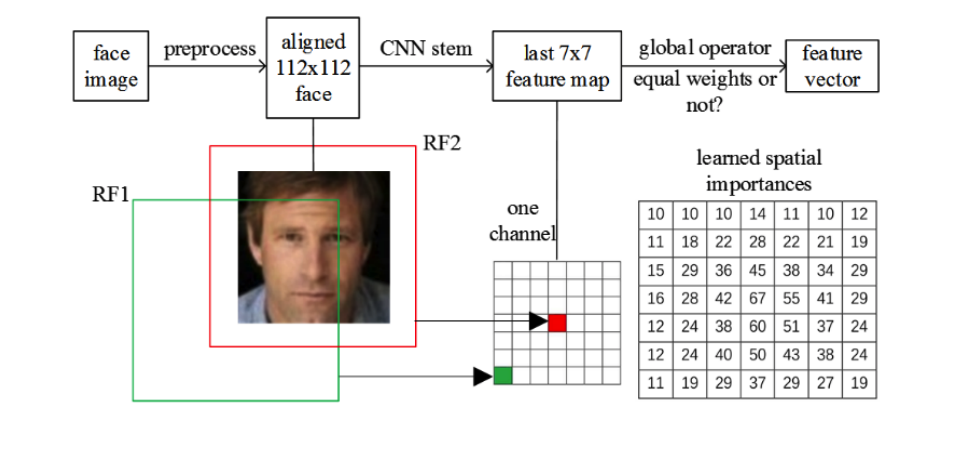
\includegraphics[width=1\textwidth]{figures/face_recognition.png}
    \caption{Face verification}
    \label{fig:face_ver}
\end{figure}

The MobileNetv2 is used similarly as in face detection up to the last feature map with size 7x7. At this step a Global Depthwise Convolution takes places, which uses a kernel of the same size as the input size. The output of this convolution is a 1x1xC while C being the number of channels. The reason behind using this approach in the last convolutional layer is that it reduces the last feature map to a vector. Which is then used as an identity for a person and the model uses it for facial recognition by computing the euclidean distance of this vector and other vectors. 



\chapter{Hyperledger Fabric for Storing Images}



In the previous chapters we have discussed how blockchain with its underlying immutable ledger can facilitate IoT and its reliance on a centralized cloud. A blockchain-based and decentralized approach could overcome the many issues associated with the centralized approach. The video surveillance monitoring system that we propose captures images once it detects a person and grants or rejects access. In order to keep evidence we store images of detected people in the Hyperledger Fabric. Considering the use case we need an additional layer of security on who is allowed to participate in the blockchain and who is allowed to see what is in the blockchain. Therefore Hyperledger Fabric solves both concerns which is in the form of permissioned and private blockchain. In this chapter we are going to show the Hyperledger Fabric architecture with its components. 


\section{Hyperledger Fabric Introduction}
Public blockchain as an immutable ledger allows for storing data in the form of transactions held by distributed network of untrusted peers and each peer can join or leave the network without any restrictions. In order to add information or create transactions normally peers ought to execute a consensus protocol which typically is a Proof of Work protocol in order to validate transactions. During this process  the peers compete for a mathematical task to be solved which require a lot of computational power, this happens everytime a new block is created. Bitcoin and Ethereum fall in this category which are considered to be public permissionless blockchains. This type of blockchain is great when transparency is required and data privacy is not a concern. 
In addition due to the consensus algorithm in public blockchains the number of transactions mined is relatively low, for example Bitcoin has an average of 7 transactions per second which makes it quite slow and energy intensive. Considering the above conditions public blockchain does not offer the possibility for a wide range of use cases. Therefore many companies often chose private permissioned blockchain over the public blockchain because they: 

\begin{itemize}
    \item concern about data privacy and confidentiality
    \item need a customizable blockchain to implement their specific use cases
    \item provide more control over the resources
    \item do not involve cryptocurrencies and provide better throughput  
\end{itemize}

Having considered our use case of video surveillance access control with face detection and recognition we found Hyperledger Fabric more appropriate than any other private permissioned blockchain. 
Hyperledger Fabric is an open source permissioned blockchain developed by Linux Foundation which has received contributions from IBM and some other companies. With its modular and configurable architecture it has become a standard for enterprise blockchain. 


\section{Hyperledger Fabric Architecture}
Hyperledger Fabric differs from other blockchains as it provides solutions to the problems in the business world. So instead of having unknown participants, it has a membership service provider that allows the ones that are permitted. Hyperledger Fabric offers a pluggable consensus mechanism instead of using Proof of Work while giving a lot of freedom to chose the algorithm by ourselves. In other words the platform is pretty flexible you will get to know more once we get to each component. Figure~\ref{fig:fabric_arch} depicts Hyperledger Fabric architecture with its key features and components which we define:
\begin{itemize}
    \item Roles in Hyperledger Fabric
     \item Membership Service Provider
     \item Certificate Authority
    \item Consensus Mechanism
    \item Chaincode / Smart Contracts 
    \item Channels
    \item Ledger and State Database
\end{itemize}
\begin{figure}[!htb]
    \centering
    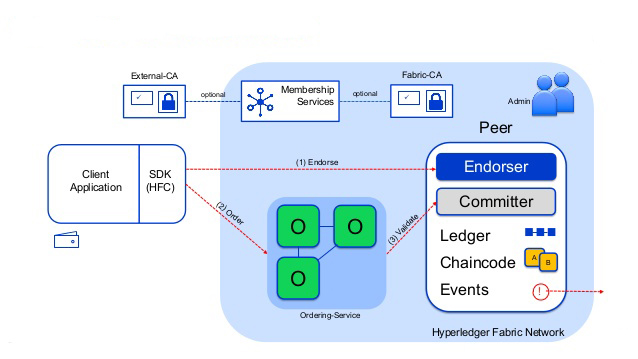
\includegraphics[width=1\textwidth]{figures/HyperledgerArchitecture.jpg}
    \caption{Fabric Architecture}
    \label{fig:fabric_arch}
\end{figure}

\subsection{Roles within Hyperledger Fabric Network}
There are a number of roles in Hyperledger Fabric but first of all the most important are the members of the organisations who operate the network and together form a consortium.
Each of the nodes that participate in the Fabric blockchain holds an identity issued by the Membership Service Provided (MSP) with each being responsible for one these roles:
\begin{enumerate}
  \item Clients or Participants. They are applications or devices that issue transactions in the network on behalf of the user. Every client is identified by the MSP and they hold certificates issued from the Certificate Authority which allows them to sign transactions.
  \item Peers. They are the fundamental element of the network because they operate the blockchain and execute transactions to the append only data structure. The blockchain ledger and smart contracts encapsulate the shared process of inserting information in the network. 
  
  \item Ordering Service. Ordering receives a transaction from the endorser it checks if the client is authorized by the MSP. If that's the case it orders the transactions in a block and delivers the blocks in atomic or total order broadcast. 
  
  \item Administrators. They stand one level above a member. They are responsible for adding or removing members from the blockchain. 
  
\end{enumerate}

\subsubsection{Types of peers: }


\begin{enumerate}
\item Endorsing Peer. In Hyperledger Fabric it is not necessary that all peers execute the transactions but only a subset of them which are named as endorsing peers. Every chaincode holds an endorsement policy, which first of all defines which peers are allowed to execute the chaincode. The endorsement policy holds from the moment the chaincode is installed on the endorsing peers. Every chaincode can specify its own endorsement policy. Each and every peer that holds that particular chaincode will have to do the endorsement and each organisation must have at least one endorser peer. The request for adding transactions comes from the client and the endorser ought to assure the client is valid, if the client has a true Certificate Authority and digital signature. 


\item Ordering Peer. 
After an order node receives a transaction from the client which is also signed by the endorser it checks if the client is authorized by the MSP. If that's the case it orders the transactions in a block and delivers the block in atomic or total order broadcast to all the peers. The task basically is to achieve consensus on the order of transactions and deliver the decision to the committer peer. 
\item Committer Peer. The committer assumes the transaction has been validated by the order and its job is to transmit the valid transactions to other peers for inclusion in the ledger. 
\end{enumerate}



\subsection{Membership Service Provider}
Unlike public blockchain in private blockchain participants in the network are identified. Hence in Hyperledger Fabric 
MSP manages identities, each  and every entity has to obtain an enrollment certificate from a Certificate Authority which is part of MSP. Since Fabric is permissioned, every interaction or messages that occur between the nodes are authenticated with digital signature. MSP is responsible for for issuing and managing credentials in order to authenticate and authorise the every node in the network. Typically there is one MSP per organisation but it is still possible to have one MSP to serve multiple organisations. In addition MSP also defines roles, access rights and the rules for each type of peer. MSP makes use of Certificate Authority which makes it easier to verify and revoke certificates when need. In other words MSP allows to find out which identity is to be trusted and which ones to be rejected. 

\subsection{Certificate Authority}

Hyperledger Fabric uses Public Key Infrastructure (PKI) for the digital identity. Each digital identity is provided with X. 509 digital certificate in order to verify that a public key belongs to the entity who owns it. The role of public private key in Hyperledger Fabric is mainly to sign transactions. When an application user initiates a transaction it first signs the transactions with his private key issued by his organisation and it also includes the public key and the signature. 

By default Hyperledger Fabric provides a Fabric-ca which is a certificate authority for handling digital identities reflected in Figure~\ref{fig:fabric_arch}. Fabric-ca is in charge of registering identities, issuing of Enrollment Certificates and renewing or revoking certificates. However Hyperledger Fabric is not bound to Fabric-ca for managing digital identities but instead it allows for external CA also. This is another proof which shows the modular nature of Hyperledger Fabric. 

\subsection{Consensus Mechanism}
Most of the public blockchains like Ethereum are permission-less which means the peers do not trust each other. In order to ensure trust on what gets registered in the ledger there is a need for consensus algorithm such as Proof of Work. However with permissioned blockchains the entities are all known and the consensus takes a different approach.  Eventhough the participants is known but the still they are not fully trusted. 

Every client that submits transactions belongs to an organisation which means that the client represent the organisation itself. Therefore in order to ensure the organisation is not doing any mischief there is a need for an agreement or consensus.   
In Hyperledger Fabric there is a need to compromise on the ordering of transactions in the block and most importantly validating those transactions in the block that will eventually be inserted in the ledger. Consensus in Fabric is broad and covers the entire transaction flow, starting from proposing a transaction till committing it to the ledger. But we need to keep in mind that transactions are executed before the ordering. For executing transactions there is no need for a consensus algorithm its the orderer peer that does it by holding to the rules in the endorsement policies applied. Consensus in Fabric ensures the correctness of of all transactions in the proposed block and agreement on the ordering of transactions. This brings to the properties which are needed to guarantee agreement between nodes: safety and liveliness. "Safety" means when a node receives the sequence of transactions to be inserted in the ledger, the same sequence and state occurs on all other nodes. "Liveliness" means even though some of the nodes may be faulty, the non faulty nodes will still be able to receive the committed transactions. 

The ordering of transactions is assigned to a pluggable algorithm for consensus which is loosely coupled to the peers that execute and maintain the ledger. This allows the organisations running the blockchain to chose the consensus algorithm that best fits their need and use case without limiting their own creativity. The component where the consensus is applied is the ordering service. 

\subsubsection{Consensus Algorithms Used in Hyperledger Fabric}

With its pluggable architecture Fabric allows developers to configure the development with the consensus algorithm which best suits the organisations needs. Currently the supported options are: 

\begin{itemize}
  \item \textbf{Solo.}  As the name says solo, the ordering service is performed by only one single peer. Clearly this is not the best option and it is neither decentralized  nor fault tolerant. But since solo is used only for development purposes there is the advantage of letting the developers focus on other matters while developing the chaincode and application and it is not used in production. 
 \item \textbf{Kafka.} The Apache Kafka provides a crash fault tolerant (CFT) but it is not Byzantine Fault Tolerant (BFT). Apache Kafka is an event streaming platform based on publisher-subscribe messaging which comes with high throughput and low latency. It follows a leader-follower model which means there will be a leader peer and follower peer. The leader will order transactions and propagated that to all other peers and if the leader goes down then re-election takes place for choosing the leader. 
 \item \textbf{Raft.} Raft is one of the latest mechanism recommend from Hyperledger Fabric which is there to improve the Kafka mechanism towards a (BFT) ordering service. Raft and Kafka provide the identical approach to the ordering service component. Both of them follow the leader and follower and design and are crash fault tolerant. However Raft overtakes Kafka by a number of major advantages worth considering. First of all Raft is much easier to setup considering that deploying Kafka with additional baggage such as Zookeeper. Secondly, Kafka is not scalable and it runs in a tight group of peers. There can be different organisations running Kafka but yet the nodes running Kafka will all go to the same cluster which is managed by a single organisation. With Raft it is possible to spread the nodes in different data centers, so if one data center becomes unavailable the other one is there to recover and continue the operation.

 
 \item \textbf{Simplified Byzantine Fault Tolerance (SBFT).} This is a new approach which is planned to be implemented by Hyperledger Fabric. SBFT is both crash fault tolerant and byzantine fault tolerant. With this approach the nodes can reach agreement eventhough there are faulty or malicious nodes. 
\end{itemize}

\subsection{Chaincode or Smart contracts}
Since Hyperledger Fabric does not support cryprtocurrencies, it however comes with the notion of "asset" which typically is a tangible good (real estate or hardware). To simplify the trade between different participants and holders of the assets there is a need for smart contract or chaincode which holds the governance rules. Literally chaincode and smart contract refer to the same thing but technically is more than a smart contract. 

Fabric uses the term chaincode to refer to a docker container which holds a group of related smart contracts. The difference is mainly in the way it is deployed in the network, smart contract manages transactions, however chaincode governs one or multiple contracts which is packaged as a single component. The deployment of chaincode takes a different approach, first it has to be packaged, then installed and only after that it can be used. Before it is installed every chaincode can specifiy the endorsement policy which defines the conditions necessary for a valid transactions. In addition the chaincode specifies the set of  endorsing peers the chaincode will be installed. This allows multiple organisations to agree on the chaincode operation before it can be used. 


During chaincode installation the endosring peers that are chosen to run the chaincode need to approve the chaincode otherwise the chaincode will not be installed. After the chaincode is installed each of the endorsing peers must endorse a transaction before it is commited. 



Since agreement happens upfront and are explicit there is no need for a deterministic chaincode. This makes Fabric exceptional because then it allows to write chaincode in a deterministic programming language. This is why Fabric allows the chaincode to be developed in Go, Java and Javascript. 




\subsection{Channels}

Channels allow the creation of sub networks within the same Fabric network. This is a huge advantage for organisations that are competitors and want to make their transactions invisible to their competitors. Channels allows the participating organisations to create and maintain their own private ledger. The ledger is not visible to any other organisations except the members participating in that channel. 
Each organisation would normally want to have their own peers in the blockchain. Suppose there are three organisations A, B and C. All of them are connected with one single Channel and maintain one single ledger. If now A want to buy a specific product from B, A do not want to share the details with C. Therefore A and B would want a new channel having their own peers. Since C is not part of channel it will not be able to see their ledger. Each channels can have one ledger only. 
Technically a channel is a subnet between two or more members.  

An endorser peer may participate in more than one channel therefore it allows them to hold two ledgers or more at the same time. 

A few features that hold: 
\begin{itemize}
  \item Every channel may have only one ledger.
  \item A channel may have one or multiply chincodes.
  \item Every chaincode has its own endorser peers and endorsement policies.
  \item A chaincode must be installed on peers that are members of a channel where the chaincode will be deployed. 
  \item One channel may have more than one chaincodes.
  \end{itemize}


\subsection{Ledger and State Database}

Like any other blockchain platforms also in Hyperledger Fabric the ledger keeps track of all important information by storing the history of all transactions. While the state of the assets may change the history behind it is immutable. In Hyperledger Fabric the ledger contains two distinct parts, the world state and the blockchain itself. 
The ledger is kept by all peers except a subset of orderers. 
Figure~\ref{fig:ledgerdiagram} shows the structure of blockchain with the blocks and the transactions in each block. Each blockchain is structured as back-linked list of blocks which include a hash of the prior block. More specifically the Block header holds the hash of the previous block as well as the hash of its own transactions. There are additional information stored in the block which can be seen in  Figure~\ref{fig:ledgerdiagram}. The transactions are stored in Block Data and the number of transactions is not necessarily the same. Each orderer assembles the transactions coming from the consensus algorithm. The conditions for creating and closing the block is based either on the maximum number of transactions allowed per block or when a timeout period has elapsed which is counted from the time the first transaction has been endorsed. 

\begin{figure}[!htb]
    \centering
    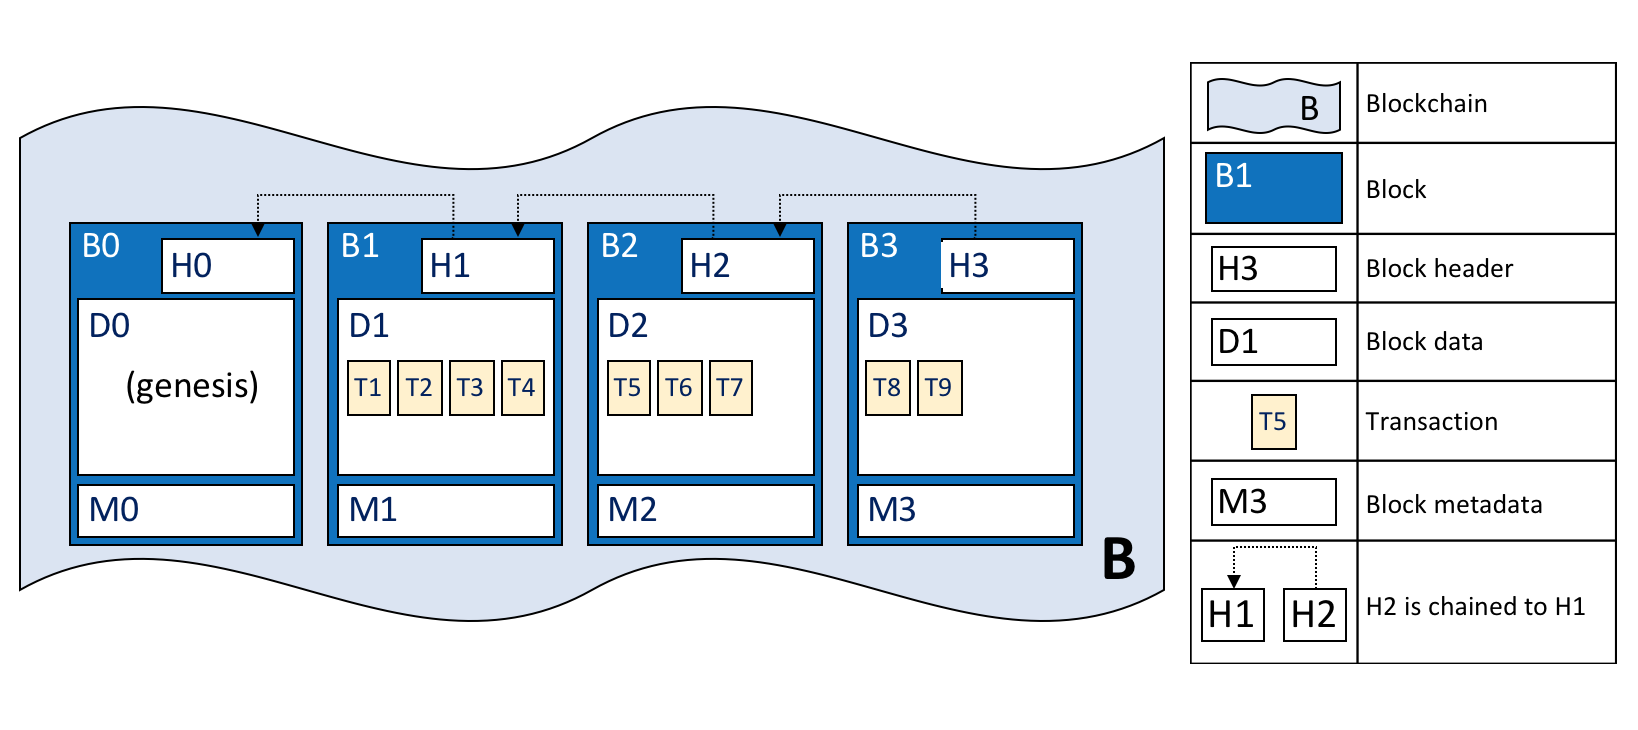
\includegraphics[width=1\textwidth]{figures/ledgediagram.png}
    \caption{The structure of the ledger.}
    \label{fig:ledgerdiagram}
\end{figure}

Blockchain data or asset in Hyperledger Fabric is represented as a collection of key value pairs. Assets can be in JSON form or binary. The state changes are recorded as a result of transaction execution in a set of key-value writes. 


In addition to the blockchain data there is a world state which represents the current state of the ledger. Word state similarly as the ledger holds a key value pair in a database which can be either CouchDB or LevelDB. With the world state the program can query the current most updated value of a state (key) without having to traverse the entire transaction log from the blockchain ledger. The world state is updated upon transaction execution and follows the consensus algorithm of the network. The approach is that only after the transaction has been signed by endorser, executed by orderer and validated will eventually result in the update of the world state. If the transaction is considered invalid and has not passed the lifecycle it will not update the world state. 

Some peers may not join the network from the beginning so for these nodes the world state will be empty. However since every new transactions represent a valid change in the world state therefore the world state can be generated easily and within some time it will be able to fully hold the latest assets' state.  
\chapter{Design and Implementation}
\label{chap:cran_for_lora}

In this section we will be elaborating and reasoning the design decisions taken in order to materialize the idea of IoT based surveillance with the blockchain technology. In the first part we will be discussing in detail the different approaches, technologies and communication protocols considered throughout the design decisions. We will also see how the IoT surveillance system with access control drives the design decisions. 

In the second part the design decisions taken will be put into action by implementing the architecture. A number of APIs and data structures are used to materialize the idea however still the Esp Eye device comes with limitations such as the max array size and due to which a dynamic memory allocation is needed.  





\section{Hardware Components}

Before digging deeper in this section we would like to describe the hardware architecture and its components involved in the project.
The video surveillance for face detection and recognition is handled by ESP EYE where the testing environment is based on an AMD Processor machine which can be Windows/Linux/Mac.
In Figure~\ref{fig:hardarchitecture} on the left hand side we have multiple Esp devices which communicate with the IoT gateway within the same network with Wi-Fi based on IEEE 802.11 standards for communication protocols. 

\begin{figure}[!htb]
    \centering
    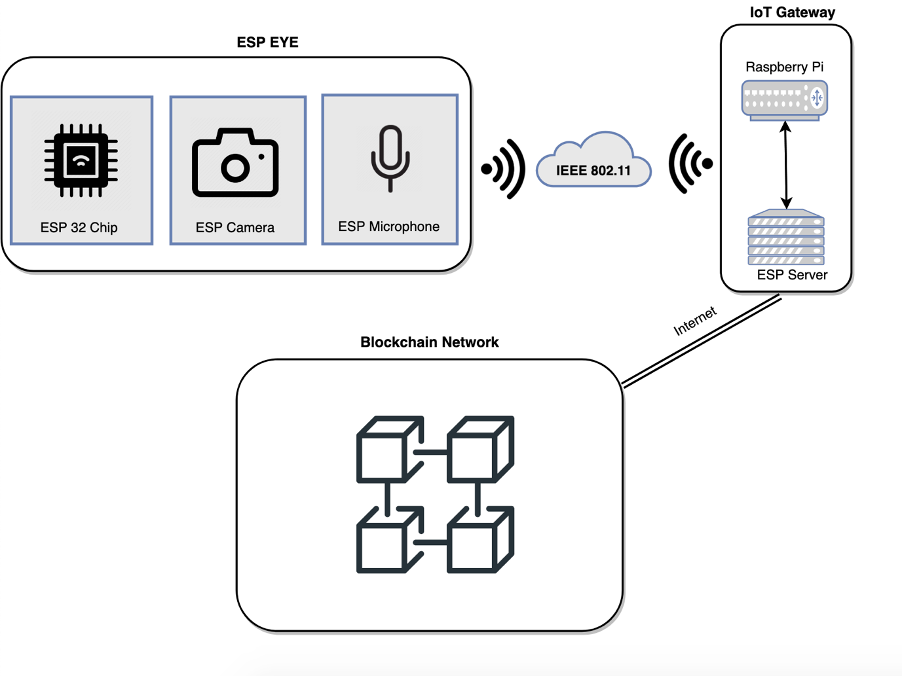
\includegraphics[width=1\textwidth]{figures/surveillance1.png}
    \caption{Hardware Architecture}
    \label{fig:hardarchitecture}
\end{figure}


The IoT Gateway serves as the middle man which waits for images coming from Esp Eye to be inserted into the blockchain. As the main experimental devices in our project we have Esp Eye and the raspberry Pi. But due to experimental purposes we had to run the blockchain locally and that lead us to change the infrastructure and instead of the raspberry pi which is an ARM based processor machine we had to go for AMD based processor machine. This is due to the Hyperledger Fabric which runs in form of containers and its binaries are only available for an AMD processor. However the architecture in the Figure~\ref{fig:hardarchitecture} still holds true. 


\subsection{Esp Eye for Face Detection}

ESP EYE which can be seen in Figure~\ref{fig:espeye} is an AI development board which is based on ESP32 chip. The device was first for sale in 2020 by the semiconductor company Espressif. There are many other devices which are based on the ESP32 family of chips. ESP32 is combine with extra components such as programming interfaces, different sensors which are used for the evaluation of the chip. 
At the core of the board is the dual core Tensilica LX6 processor with 8 MB PSRAM and a 4MB flash. 

The Esp Eye integrates an embedded microphone and a camera with 2-Megapixels. The camera is an OV2640 sensor with a maximum image size of 1600×1200 pixels. The board supports  2.4 GHz Wi-Fi technology to connect to internet through a wide area network. A Micro USB port provides the power supply and also debugging in order to use the AI APIs. It comes with an UART Chip which enables asynchronous serial communication with which the program is uploaded bits by bits. 
\begin{figure}[!htb]
    \centering
    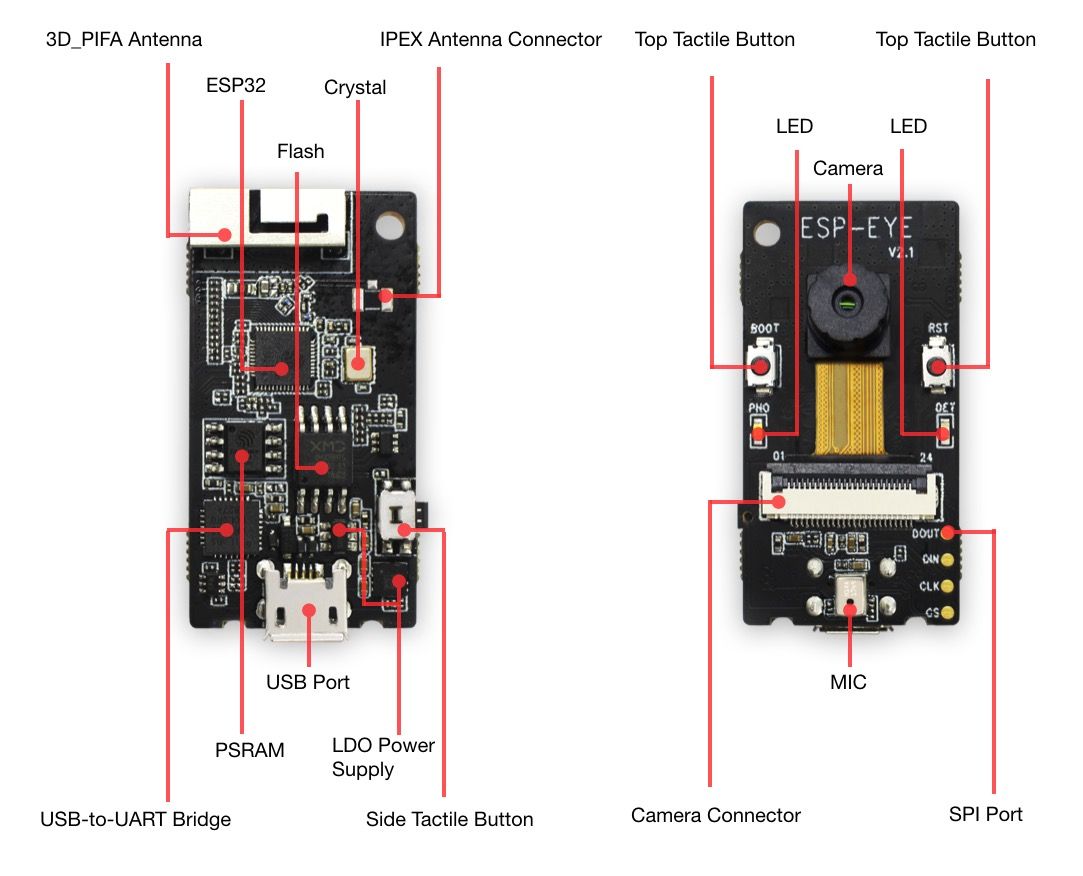
\includegraphics[width=1\textwidth]{figures/espeye.png}
    \caption{Esp Eye \cite{espeyeimage}.}
    \label{fig:espeye}
\end{figure}


Esp Eye also supports additional security features: flash encryption feature and secure boot. The flash encryption is intended to secure the content of the flash memory. In Esp Eye flash encryption is done using AES-256 and the key is stored in the eFuse. eFuses keep the values intact and can not be changed by a software. Since the data in flash is encrypted upon reboot the physical readout will be impossible. 
On the other hand secure boot can protect the device from uploading unsigned code. The algorithm is a typical digital signature method with RSA, the public is stored in the device itself whereas the private is kept secret and used upon each code upload. 

What makes the Esp Eye stand out of the crowd is its performance and the platform for face detection and recognition known as Esp-Who. Esp-who comes with algorithms for face detection and recognition which makes it possible to run both in Esp Eye.

\subsection{Raspberry PI}

Raspberry Pi has been the development environment from the beginning of the project. It is very lightweight, supports many compilers and makes it ideal for experimental purposes. Throughout this project we have been using Raspberry Pi 4 Model B, with 8GB of RAM with  integrated 802.11 wireless LAN. It worth mentioning that the Raspberry Pi is backed by an ARM processor. 
The esp32 family of devices are natively compiled and developed by the esp idf development platform.  Similarly also the Esp-Who libraries for face detection and recognition were available in esp idf development platform.
However after many tries to setup Hyperledger Fabric in Rasperry Pi we realized that Hyperledger Fabric binaries were not possible to run in ARM processor. Therefore after that a computer with AMD processor was used. 






\section{Design}

 


\subsection{Surveillance System Architecture}

Figure~\ref{fig:surveillance2} shows a high level overview with the sotware components. It is important to mention that the design is compatible without any technological restrictions. At the beginning there were two approaches in mind: deployment of face detection and recognition on the cloud or deployment in the Esp Eye device itself. In the first approach AI is deployed on the cloud which means the camera consequently captures images and send them on the cloud for face recognition. This approach is costly, based on the previous studies in average the time required to detect a person is between 2 to 5 seconds. In addition it requires substantial amount of bandwidth which would be wasted if no one is present.

In the second approach which we decided to implement the face detection and recognition run on the IoT device itself. This approach has a lot more benefits, first of all the images are captured by a very small devices powered by AA batteries. Compare to the previous approach they needed a machine on the cloud and a separate camera, whereas in this case both are converged into one single low powered device. When images are captured they are immediately detected and recognized. Which means that it can also be optimized to delete images when a face is not detected. 



\begin{figure}[!htb]
    \centering
    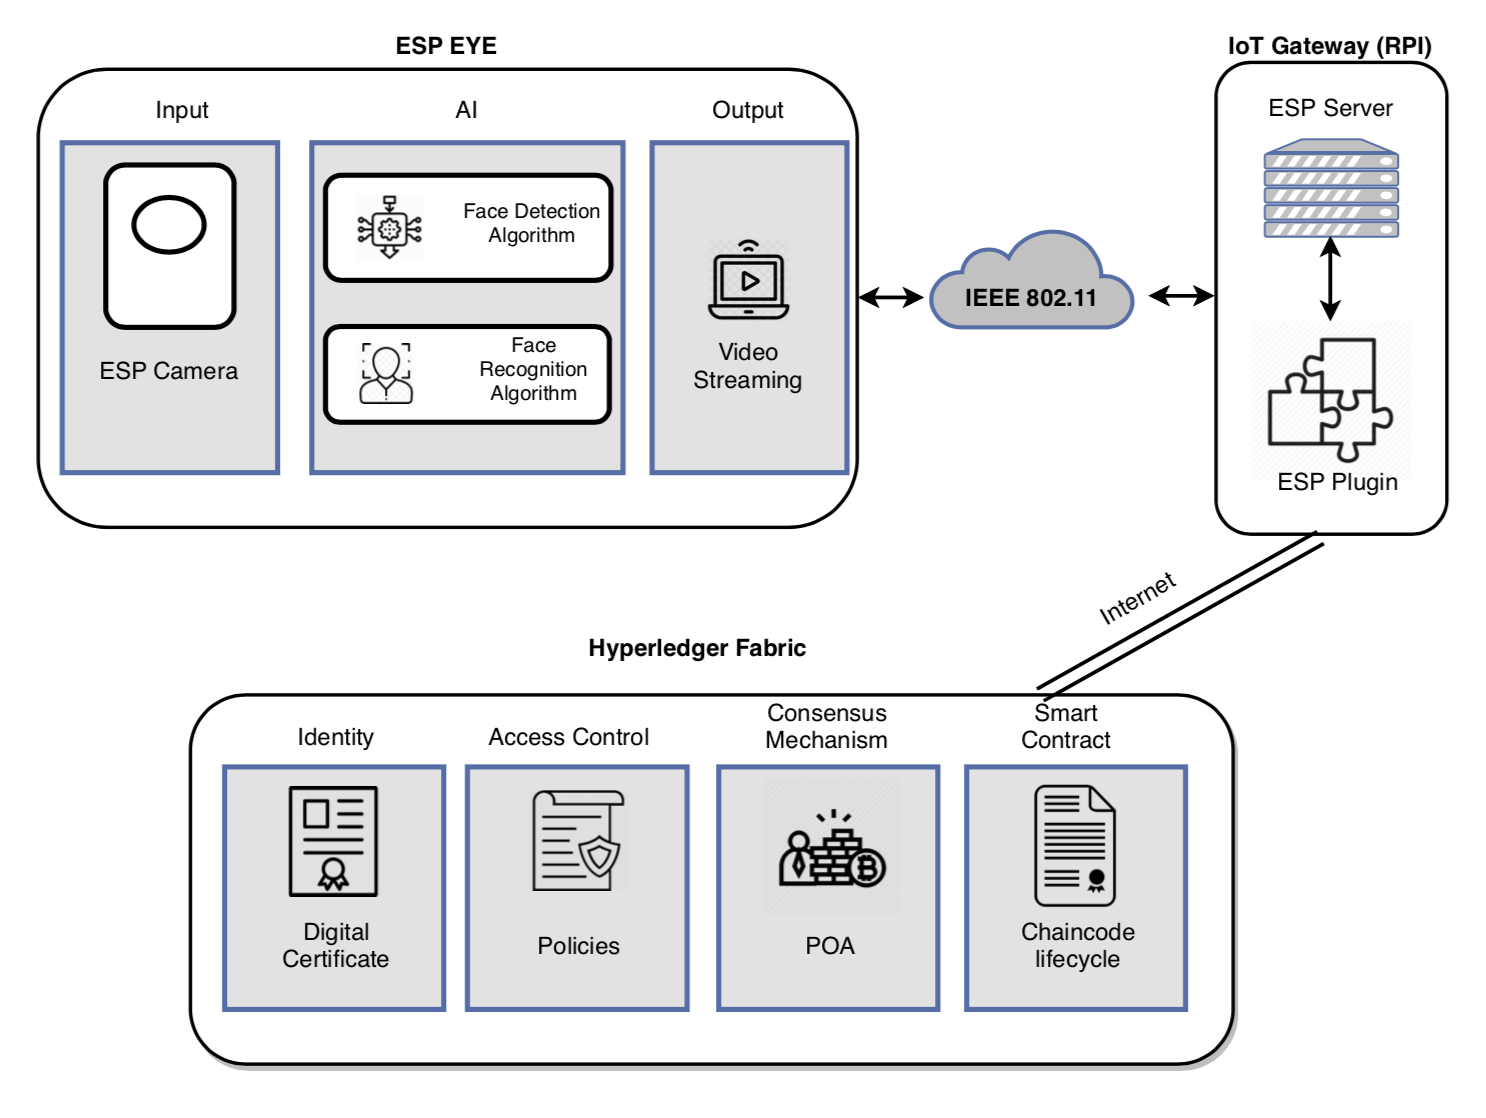
\includegraphics[width=1\textwidth]{figures/esp2.png}
    \caption{Software Architecture}
    \label{fig:surveillance2}
\end{figure}


On the right hand side of the Figure~\ref{fig:surveillance2} is the IoT Gateway which serves as a hub to do the rest of the job. The communication between the Esp Eye and the IoT gateway is achieved with a wireless communication compliant to IEEE 802.11 LAN protocols. It follows the client-server architecture, the Esp Eye is the client and the IoT Gateway as a server. Since we want to store the detected images in the blockchain having the Esp Eye as a client fulfills the requirements. The server will be waiting for requests coming from the Esp Eye. The other way around would not work, since the only way to send data from the server is when the client has sent a request. The first condition for the image to be stored in blockchain is that the face has to be detected in that image. On the other hand ESP Plugin with the help of the SDK from Hyperledger Fabric will start the process of submitting the transaction to the ledger. Hyperledger Fabric enables the storage of the detected images coming from the Esp Eye.   

\subsection{Communication Protocols under consideration}
When it comes to decision which communication protocol to use in IoT device, it is important to go for a lightweight protocol and among our choices is HTTP and MQTT both of them supported by Esp Eye with the help of IPEX antenna which enables the Wi-Fi connectivity. MQTT is an extreme lightweight protocol which follows the publish/subscribe model for communication. Whenever a client pushes a message on a subscribed topic then the message will be forwarded to all the clients participating on that topic. Due to the use case where the esp eye devices do not have to communicate in between the MQTT leaves behind. 
Instead HTTP protocol is employed where Esp Eye and the IoT Gateway communicate in the client server architecture respectively. For the inter-machine communication the REST architectural style will be used because anyways we do not want to bind the communication since we do not know when the face will be detected. Besides REST is considered to be more lightweight compare to its counterparts. For the data-interchange format the JSON format is employed which is very lightweight and performs much better since its syntax follows the javascript language so it makes it faster to read since the ESP server is also written in javascript.  
\subsection{Face detection and recognition algorithms in Esp Eye}
Although very small in size the Esp Eye still stands out of the crowd because of its features and communication standards. With 8 MB of PSRAM and 4 MB and Wi-Fi transmission of flash it gives room for deploying ESP-WHO a platform and a library for face detection and recognition. ESP-WHO is a framework and library which provides the face detection and recognition algorithms. It is developed using the ESP IDF an SDK with software development tools which includes compiler, debugger and some plugins to integrate with additional IDEs.  ESP IDF contains the essential software libraries for the face detection with MTCNN and MobileNets model and face recognition libraries implemented with MobileFaceNet model. In order to elaborate how face detection and recognition works we have Chapter 3 which explicitly explains the used models. 

Although we could have used ESP IDF development environment but rather we chose to develop it in Arduino IDE. Arduino IDE provides a lot of libraries including the libraries for ESP32 boards. 



\subsection{Hyperledger Fabric a tamper-resistant database}

  The main criteria were that the blockchain ought to be private and permissioned since the images should not be public and only available from within the organisation that applies our use case. Ethereum and Hyperledger Fabric was another potential candidate to be deployed.Among the two we decided for Hyperledger Fabric because from the beginning it is meant to be private permissioned blockchain. Although Ethereum can be adapted to serve our needs but yet it comes with a consensus mechanism which is energy demanding and not flexible. Hyperledger Fabric provides a modular architecture and enables more flexibility and is tailored to the needs of our use case. For a better undestanding of the architecture of Fabric you can refer to Chapter 4.  Hyperledger Fabric in our case stands out of the crows due to its features: 

\begin{itemize}
    \item High transaction throughput
    \item Low latency for transaction confirmation
    \item Confidentiality of transactions with the help of channels
    \item Highly modular architecture
    \item Identities supplied with digital certificate 
\end{itemize}

With its modular architecture it allows to be tailored to the needs and the use case. It has been designed to be highly configurable and offers modularity for the following components: 

\begin{itemize}
    \item A pluggable consensus or ordering service which is the core component for transection execution.
    \item A pluggable Membershi Service Provide responsible for managing entities and associating them with cryptographic information.
    \item A pluggable Certificate Authority responsible for issuing and managing the identities with digital signature cryptography.
     \item A smart contract implemented in a conventional programming languages known to developers. 
    
\end{itemize}



\section{Implementation}

The first part of the chapter elaborates the design decisions and the network communication decisions. Therefore in this section we will show what it takes to implement the above mentioned design decisions. First the data flow will be discussed on how data flows from esp eye devices until it reaches the Hyperledger Fabric. Secondly we will show how the transaction is originated from esp eye and the way it takes to until it is executed and validated to eventually be stored in the ledger.  

\subsection{Data Flow Overview}

In this setup the Esp Eye devices and the IoT Gateway are all connected in LAN and operate within the same subnet. In Figure~\ref{fig:dataflow} the Data Flow Diagram is depicted which shows the flow from left to the right starting with the Esp Eye. Esp devices act as stations and the reason is that there are multiple esp devices and it would not be a good choice since the Hyperledger Fabric libraries for transaction instantiating are not available in Esp Eye if we were to endorse the transaction from Esp Eye. Once Esp Eye detects a face or eventually recognizes who that person is it will take that exact image and forward it to the IoT Gateway. This is achieved with a REST API call using the POST request where the image is included with additional metadata. On the other hand the nodejs server located in the IoT Gateway will receive the request in our case the image with  a detected person and forward the image to Hyperledger Fabric. 

\begin{figure}[!htb]
    \centering
    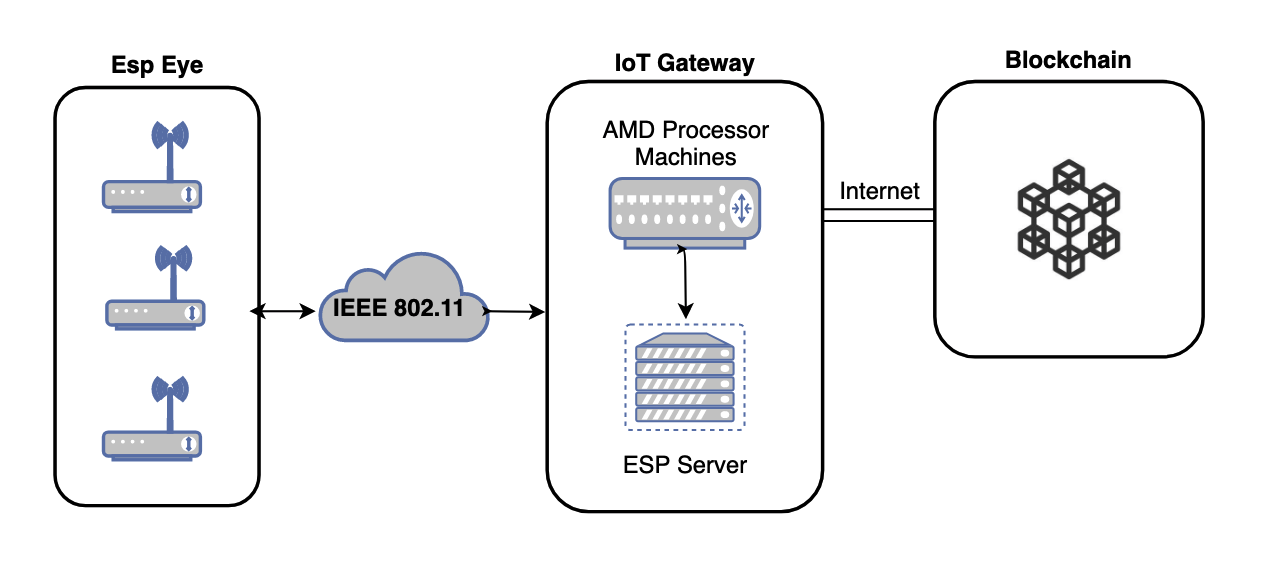
\includegraphics[width=1\textwidth]{figures/dataflow.png}
    \caption{Data flow diagram}
    \label{fig:dataflow}
\end{figure}
The nodejs server is responsible for receiving the data and forwarding it to the Hyperledger Fabric. 
In order to interact with Fabric blockchain network the Fabric SDK for nodejs provides us with APIs to submit transactions to the ledger. The process of submission takes place right after the image has arrived. Hyperledger ledger data is known as assets which are represented as as a collection of key-value pairs. When the value of the key is modified by a chaincode simulated from transaction execution then the world state is updated as a new transaction on a ledger. Assets written by chaincode typically use the JSON form and or binary. Since for the backend the JSON format is used for file transfer then this allows for sending the same JSON parameters to the blockchain. The role of nodejs server is to receive and acknowledge the Esp Eye that data has arrived and then forward the exact same data to the blockchain. The process begins with transaction initiation where Esp Eye is assumed to be a client and such that it holds an identity issued from the MSP. 

A question may arise why are we storing the image directly in the blockchain. First Hyperledger Fabric runs at no costs for transaction execution and the consensus mechanism is very lightweight and pluggable. Secondly, since Hyperledger Fabric allows for splitting the network into multiple smaller networks in order to preserve privacy between competitors then storing images in some other third party such as IPFS would vaporize the concept of channeling and IPFS does not offer the same characteristics. 


\subsection{Transmission Overview}
\subsubsection{Esp Eye starts video surveillance}
The data transmission is depicted in Figure~\ref{fig:seqdiag} which captures the interaction between all the components end to end. When an Esp Eye device established connection to the LAN it then immediately start the process of video surveillance. Roughly it takes 4 frames per second and analysis each frame for face detection and if a face is detected only then it puts into work the face recognition algorithm. Only if a face is detected or eventually recognized the client code will be activated and eventually through an end point using the POST method. 






\begin{figure}[!htb]
    \centering
    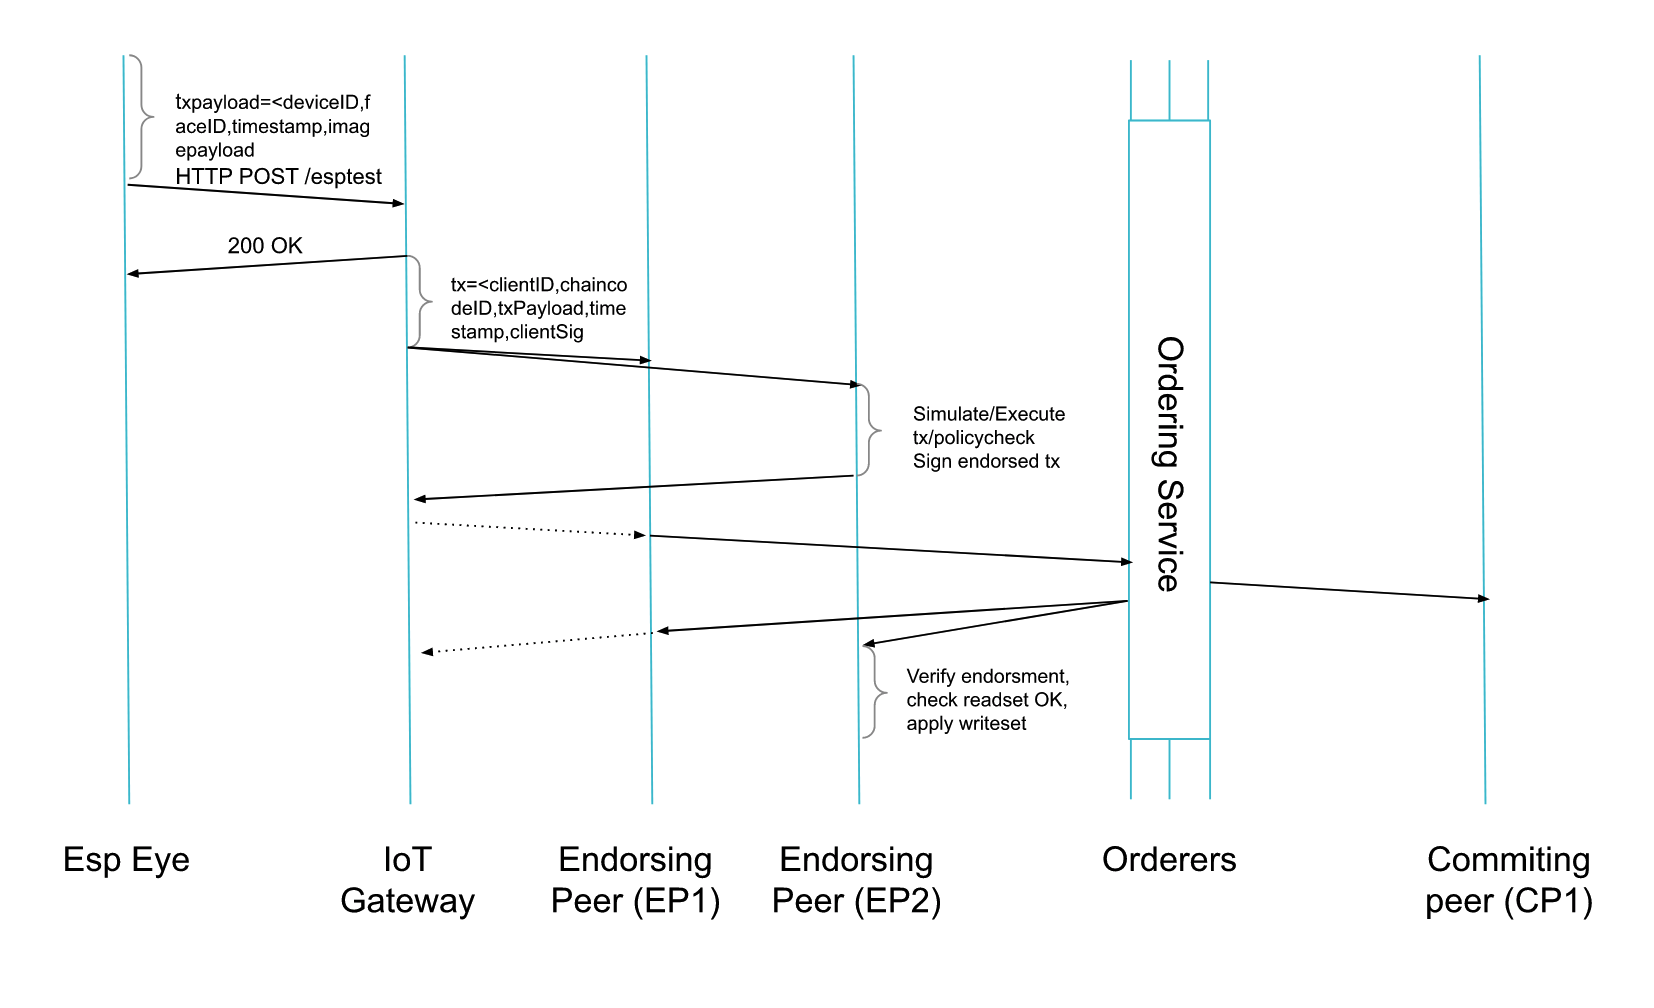
\includegraphics[width=1\textwidth]{figures/sequencediagram1.png}
    \caption{Sequence Diagram showing transaction execution}
    \label{fig:seqdiag}
\end{figure}




There are 4 important information needed to be stored in the blockchain and are reflected in the Figure~\ref{fig:json}. First the DeviceID is important since we need to know from which device is this information coming as multiple devives may be employed in video surveillance. Secondly with FaceID we will be able to identify the person without having to look on the captured frame. Additionaly with timestamp we capture the time when the person is detected and finally the frame itself encoded in base64. 

As in Figure~\ref{fig:seqdiag} these 4 parameters will be sent first through the exposed API with an endpoint /esptest. The nodejs server located in IoT Gateway will then reply with the status code but no additional information. 

\begin{figure}[!htb]
    \centering
    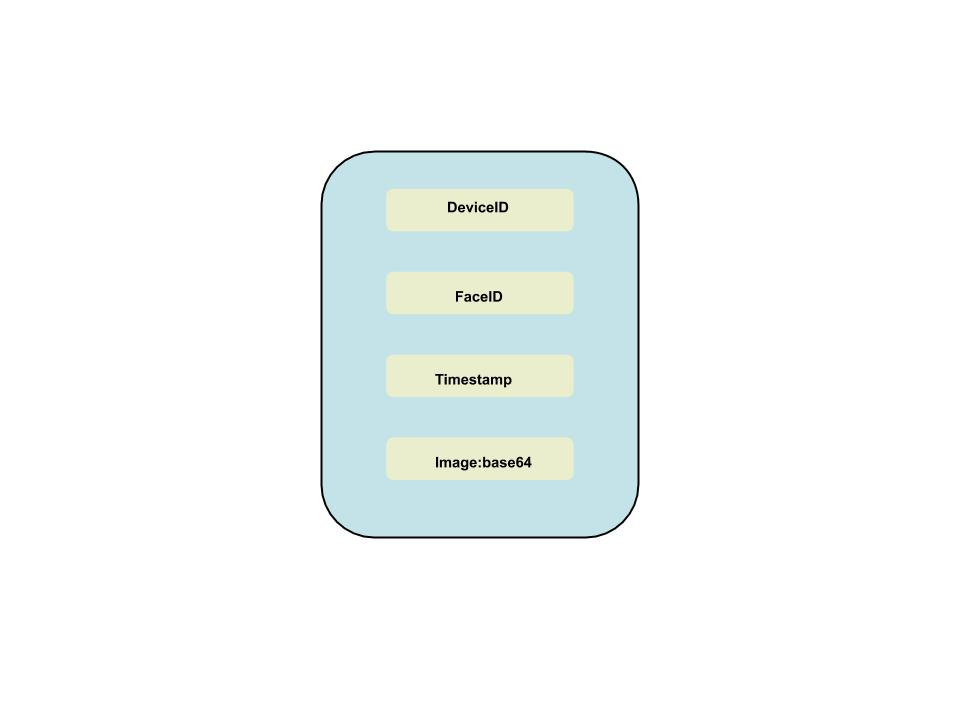
\includegraphics[width=1\textwidth]{figures/json2.jpg}
    \caption{JSON parameters sent from Esp Eye}
    \label{fig:json}
\end{figure}
\subsubsection{IoT Gateway initiates a transaction}
Before transaction is initiated there are three assumptions necessary to keep in mind:
\begin{itemize}
    \item The channel in Fabric is running.
    \item The Esp Eye is registered and enrolled with Certificate Authority and MSP holds its identity.
    \item The chaincode with its endorsement policy is deployed on the peers.
\end{itemize}


Now the job of the IoT Gateway is to initiate the transaction with the 4 paremeters passing them as they are to the transaction payload. The IoT Gateways acts as a Fabric client for Hyperledger Fabric. Our endorsement policy states that both peers taking part in the consortium must endorse any transaction coming from this client. The transaction proposal now is easy constructed, since Fabric holds assets in key value pairs in our case the key will be the FaceID and all other information will be stored in a json document as values. This will make it easier to query the FaceIDs and for the world state. The transaction proposal utilizes an API for nodejs SDK to generate a transaction. The goal of the API which we are going to see its implementation soon is to invoke the functions of the chaincode with input paramters coming from Esp Eye. Each Esp Eye is issued a public private key pair which is used to sign the transaction before sending it to the endorsers for execution. In this case the Fabric-client SDK persists the public private key and signs the transaction on behalf of the Esp Eye. Although transaction signing is possible in offline mode which means the user signs the transaction at his device and sends the signed transaction to the endorser node. In our case this was not possible since the Fabric-client SDK is not available for Esp Eye devices. 

\subsubsection{Endorsing Peers EP1 and EP2 verify and execute the transaction}

The endorser EP1 and EP2 from Figure~\ref{fig:seqdiag} will now receive the transaction proposal which includes: clientID, chaincodeID, txPayload, timestamp and clientSignature as in Figure~\ref{fig:endorsejson}. Only the endorsing peers specified by the chaincode will receive this transaction proposal in our case both of them will receive a proposal. EP1 and EP2 first of all check the format of the transaction and if the signature is valid and if that is the client who claims to be using the MSP. Besides it also ensures that this client in this case Esp Eye is an authorized member of that channel. When all the conditions have passed then the endorses invokes the chaincode function and pass the four proposed arguments. Eventually the transaction is executed however it does not yet update the ledger. Now the endorsers sign the proposed transaction and send back a proposal response to the fabric-client. The intent of the fabric-client now is to submit the transaction to the ordering service to update the ledger. If the fabric-client was to query the ledger then there is no need to submit anything to the ordering service. However in order for the fabric-client to submit the transaction to the ordering service both endorser EP1 and EP2 have to respond with same response proposal. However yet at this stage the ledger is not updated. 

\begin{figure}[!htb]
    \centering
    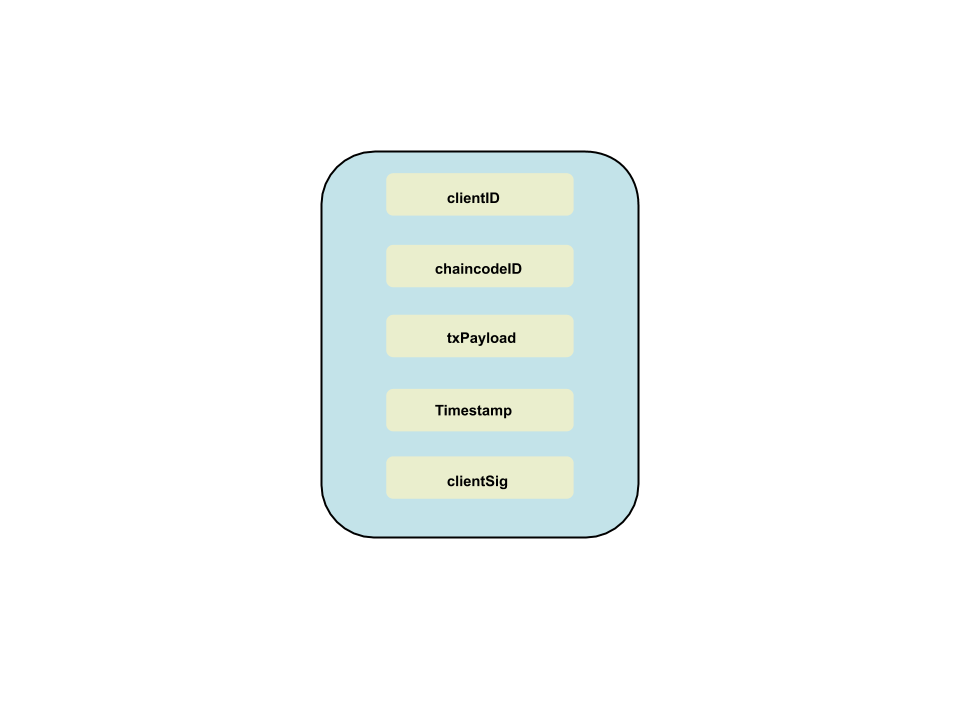
\includegraphics[width=1\textwidth]{figures/endorsejson.png}
    \caption{Proposed transaction with its parameters.}
    \label{fig:endorsejson}
\end{figure}


\subsubsection{Fabric-client submits transactions to the ordering service}

Before the fabric-client submits the final version of the transaction, the application broadcasts the endorsed transaction with a message to the ordering service.
The transaction proposal now will contain the read/write sets besides the endorsing peers signatures. 
The ordering service nodes may receive transaction from other clients or other ESP devices. The job of the ordering service is to order transactions on an agreed sequence in order to package them into blocks. After the maximum number of transactions allowed in a blocks is reached or the maximum time duration has passed then blocks are saved first to the ledger of the orderers. 


\subsubsection{Validate and commit the transactions to all peers}

Upon receiving a broadcast message with the created block from the orderers the committing peers will again verify the signatures of the ordering nodes which are part of the ordering service. In Fabric it is allowed to set which peers will validate the transaction and they are name as committing peers, however all the peers in the channel ought to update the ledger.
If the committing peers fail to verify the signature of the ordering peers that created the block then the block is rejected for inclusion in the ledger. Another very important validation step is to ensure that every transactions' read and write set does not lead to invalid world state. During the endorsement phase the every transaction copies a set of read and write sets of the key pair that will get updated. Hyperledger Fabric in addition to key value pairs it implicitly keeps the third parameter which is the version number of that pair. When a new transaction is executed the versioning  of the key pair gets updated, it is like a counter. The read set comes from the world state and the write set is the same key but with updated value and version. In our case the key will be the FaceID and the value is the new image.

The committing/validating peers will now verify the transaction by looking at the read write sets. Now the committing peer will compare the read set it holds with the world state of the same key. If the versioning of the key does not match then a previous transaction could have updated and the version is also updated which means the transaction will be considered invalid and will be rejected from the block. This is how it prevents the double spending. Otherwise if the read set and its version has not been changed the transaction is then allowed to be inserted to the ledger. Eventually the write sets are committed to the world state and the detected image has reached all the peers. 
 
 \subsubsection{Execution model}
 
 
 Typically the permissioned blockchains such as Ethereum, the transaction is executed by all peers in the block level which means that the consensus protocol first orders the transactions and propagates to the peer nodes and only then the execution of transactions takes place. Therefore they operate in order-execute-validate model. The execution happens after all the transactions have been propagated to all peers by executing sequentially all the transactions in all peers.
 
 Unlike the traditional approaches, Hyperledger Fabric follows the execute-order-validate model which is reflected in the above described steps. This model has a lot of advantages. First of a transaction is not executed by all the peers but only by a subset of the peers. Besides also the transaction endorsement and validation may be executed only by a subset of the peers which means not all the peers need to execute the chaincode. Since many peers are released from the transaction execution this can save energy and resources because some of the peers may be running far away from each other. 
 This approach uses a non-deterministic chaincode because the peer agreement is explicit  which allows to implement the chaincode in a non-deterministic programming language. In addition the Fabric allows to execute transactions in parallel in order to increase throughput. Besides the elapsed timeout for a block creation makes Hyperledger Fabric much more efficient for transactions coming from IoT devices.
 
 
 
\subsection{Esp Eye Setup}

In the previous section with a sequence diagram the data flow from one object to another is elaborated. In this section we would like to stop on the most important parts of the implementation for face detection and recognition which is entirely implemented using Arduino IDE. Since three domains are involved we wouldn't be able to elaborate all the details here because the focus is merely on the interactions between them. Because of that the face detection and recognition algorithms implemented in Esp Eye are shown in more detail in Chapter 3. Therefore we will now take a look at the most important parts of implementation which runs face detection and recognition.

%First of all the implementation begins with setting the GPIO parameters in order to connect to camera. This is important because each ESP32 camera board uses different GPIOs. Now we would like to fave a close look at the APIs used for face detection and recognition.

\subsubsection{Face Detection API} 

First of all we would like to start with introduction to the API for face detection: {\fontfamily{ccr}\selectfont face\_detect} which is adapted from ESP WHO platform, its implementation is shown in the Listing \ref{face_detect}. As it can be seen the function returns a pointer of type {\fontfamily{ccr}\selectfont box\_array\_t} which contains information about the face such as the bounding box and the face landmarks. When no face is detected the function returns {\fontfamily{ccr}\selectfont NULL}. In our code we just check if the the function returns {\fontfamily{ccr}\selectfont NULL} then do not proceed for face recognition. The {\fontfamily{ccr}\selectfont face\_detect} function accepts to inputs of type {\fontfamily{ccr}\selectfont dl\_matrix3du\_t} and {\fontfamily{ccr}\selectfont mtmn\_config\_t}. 


\begin{lstlisting}[caption={Face detection API},label=face_detect, captionpos=b]

// Adapted from ESP-WHO Platform
 box_array_t *face_detect(dl_matrix3du_t *image_matrix, mtmn_config_t *config)
{ 
    net_config_t pnet_config = {0};
    pnet_config.w = 12;
    pnet_config.h = 12;
    pnet_config.threshold = config->p_threshold;
    box_array_t *pnet_boxes = NULL;
    if (FAST == config->type)
        pnet_boxes = pnet_forward_fast(image_matrix,
                                       config->min_face,
                                       config->pyramid_times,
                                       &pnet_config);
    else if (NORMAL == config->type)
        pnet_boxes = pnet_forward2(image_matrix,
                                   config->min_face,
                                   config->pyramid,
                                   config->pyramid_times,
                                   &pnet_config);
    if (NULL == pnet_boxes)
        return NULL;
    net_config_t rnet_config = {0};
    rnet_config.w = 24;
    rnet_config.h = 24;
    rnet_config.threshold = config->r_threshold;
    box_array_t *rnet_boxes = rnet_forward(image_matrix,
                                           pnet_boxes,
                                           &rnet_config);
    dl_lib_free(pnet_boxes->box);
    dl_lib_free(pnet_boxes);

    if (NULL == rnet_boxes)
        return NULL;
    net_config_t onet_config = {0};
    onet_config.w = 48;
    onet_config.h = 48;
    onet_config.threshold = config->o_threshold;

    box_array_t *onet_boxes = onet_forward(image_matrix,
                                           rnet_boxes,
                                           &onet_config);
    dl_lib_free(rnet_boxes->box);
    dl_lib_free(rnet_boxes);
    return onet_boxes;
} /*}}}*/
\end{lstlisting}






The Listing \ref{image_matrix} shows the definition of the image\_matrix a 3 dimensional matrix with the image and additional metadata about the image unlike the {\fontfamily{ccr}\selectfont box\_array\_t} which only holds features about the face. These are information about the image width, height, number of channels, number of filters, stride and a pointer to image data. Since we are dealing with a memory constraint device typically the dynamic memory allocation is used. It allows for more efficient memory allocation and the memory is not wasted. So first the memory is dynamically allocated and then the captured image is assigned to it. 




\begin{lstlisting}[caption={Image matrix structure},label=image_matrix, captionpos=b]
typedef struct
{
    int w;      /*!< Width */
    int h;      /*!< Height */
    int c;      /*!< Channel */
    int n;      /*!< Number of filter, input and output must be 1 */
    int stride; /*!< Step between lines */
    uc_t *item; /*!< Data */
} dl_matrix3du_t;

\end{lstlisting}


The second parameter {\fontfamily{ccr}\selectfont mtmn\_config\_t} also shown in Listing \ref{mtmn} is a struct which holds configurations about the MTMN, the multi stage algorithm for face detection which is explained in detail in Chapter 3. There are a number of properties which are important because they can affect the performance of MTMN and also the processing speed. The first property is 
{\fontfamily{ccr}\selectfont min\_face} which is the minimum detection size which by default is set to 80. It means that it should be able to detect all faces larger than 80x80 pixels. This property is important since we do want to detect individual faces and anyone standing in the background is not important. Therefore the smaller the {\fontfamily{ccr}\selectfont min\_face} is : 

\begin{itemize}
    \item the larger the number of images is generated in image pyramid;
    \item the higher the processing time;
     \item the smaller the size of detectable face is in the image;
\end{itemize}


In other words it means the MTMN will work harder to try to detect the face if the person is standing pretty far away from the camera. 
The {\fontfamily{ccr}\selectfont pyramid} holds the scale which monitors the generated pyramids with a range from 0 to 1. 

Therefore the larger the {\fontfamily{ccr}\selectfont pyramid} is : 
\begin{itemize}
    \item the higher the number of images generated in the image pyramid;
    \item the higher the processing time;
\end{itemize}

The {\fontfamily{ccr}\selectfont pyramid\_times} is another property which together with {\fontfamily{ccr}\selectfont pyramid} monitor the image pyramid. In addition the configuration also allows to set the threshold for each stage of the MTMN reflected in the struct {\fontfamily{ccr}\selectfont threshold\_config\_t}. The closer to 1 the lower the number of potential candidate bounding boxes and such the lower the probability of detecting a face. 
The struct {\fontfamily{ccr}\selectfont mtmn\_resize\_type} allows to chose between FAST and NORMAL. When it is set to FAST the {\fontfamily{ccr}\selectfont pyramid} equals 0.707106781. If we want to set out own value of {\fontfamily{ccr}\selectfont pyramid} the it has to be set to NORMAL. By FAST it means the processing time is faster compare to NORMAL. 


\begin{lstlisting}[caption={MTMN configurations },label=mtmn, captionpos=b]
 typedef struct
    {
        float min_face;                 /*!< The minimum size of a detectable face */
        float pyramid;                  /*!< The scale of the gradient scaling for the input images */
        int pyramid_times;              /*!< The pyramid resizing times */
        threshold_config_t p_threshold; /*!< The thresholds for P-Net. For details, see the definition of threshold_config_t */
        threshold_config_t r_threshold; /*!< The thresholds for R-Net. For details, see the definition of threshold_config_t */
        threshold_config_t o_threshold; /*!< The thresholds for O-Net. For details, see the definition of threshold_config_t */
        mtmn_resize_type type;          /*!< The image resize type. 'pyramid' will lose efficacy, when 'type'==FAST. */
    } mtmn_config_t;
    
\end{lstlisting}
%and then we will see each arguments are expected for face detection. 

In the Listing \ref{face_detect}  of the {\fontfamily{ccr}\selectfont face\_detect} function the three stages of MTMN are implemented. As discussed in Chapter 3 in the p-net stage the input image size is 12x12 this is reflected with assigning the {\fontfamily{ccr}\selectfont pnet\_config.w} and {\fontfamily{ccr}\selectfont pnet\_config.h} to 12. Similarly this happens for r-net and o-net where the width and height is set to 24x24 and 48x48 respectively. Once the function has reached the end it will return either NULL if no face is detected or else will return the bounding box, the score and landmarks.


\subsubsection{Face Recognition API} 

The input for face recognition is only the bounding box or the aligned face with landmarks for the position of eye,nose and mouth. The {\fontfamily{ccr}\selectfont recognize\_face} function accepts two parameters, the {\fontfamily{ccr}\selectfont face\_id\_list} and the {\fontfamily{ccr}\selectfont aligned\_face}.
\begin{lstlisting}[caption={Face Recognition API},label=face_rec, captionpos=b]
int8_t recognize_face(face_id_list *l, dl_matrix3du_t *algined_face);
\end{lstlisting}

The face id list also shown in Listing \ref{face_id} has a number of parameters that keeps track of the face ids, where the most important information about the face is stored in a 3 dimensional vector {\fontfamily{ccr}\selectfont id\_list}. 





\begin{lstlisting}[caption={Face Id List},label=face_id, captionpos=b]
typedef struct
  {
        uint8_t head;            /*!< head index of the id list */
        uint8_t tail;            /*!< tail index of the id list */
        uint8_t count;           /*!< number of enrolled ids */
        uint8_t size;            /*!< max len of id list */
        uint8_t confirm_times;   /*!< images needed for one enrolling */
        dl_matrix3d_t **id_list; /*!< stores face id vectors */
    } face_id_list;
    
    \end{lstlisting}

The job of {\fontfamily{ccr}\selectfont recognize\_face} function is to generate a new {\fontfamily{ccr}\selectfont face\_id} from the {\fontfamily{ccr}\selectfont aligned\_face} parameter. The newly generated {\fontfamily{ccr}\selectfont face\_id} will then be compared with all the face ids stored in the {\fontfamily{ccr}\selectfont face\_id\_list}. With the help of Cosine similarity we can measure how similar two vectors are. The Cosine similarity will then obtain the distance between the newly generated {\fontfamily{ccr}\selectfont face\_id} with each {\fontfamily{ccr}\selectfont face\_id} stored in the {\fontfamily{ccr}\selectfont face\_id\_list}. The closer the Cosine value to 1 the higher the match between two vectors and vice versa. As a matter of fact it is almost impossible to have a Cosine value 1 of two compared faceIDs. This is challenging due to image differences in terms of light, pose and facial expression. Due to that we can set a threshold {\fontfamily{ccr}\selectfont FACE\_REC\_THRESHOLD}  to either increase or decrease the recognition rate. When it obtains a Cosine value greater than the threshold when comparing two face IDs then it is considered to be the same person. 

\subsubsection{Sending detected image to IoT Gateway} 

The image is sent to IoT Gateway either when a face is detected or recognized. The WiFiClient library in Arduino enables to establish the connection to the IoT Gateway by using the IP address of the IoT Gateway. The Esp Eye makes an HTTP request using the POST method through an exposed API from the IoT Gateway. Throughout this study for submitting the image to the IoT Gateway two ways were used: 
\begin{enumerate}
    \item multipart/form-data
    \item application/json
\end{enumerate}

With "multipart/form-data" the image is sent in series of parts. This approach allows to send a file or image without looking at its type. This approach was used at the beginning of the project implementation when a python server was used and such that we did not have information about the Hyperledger Fabric implementation which uses Javascript for interaction with blockchain. This approach is beneficial when we do not want to capture the raw image in bytes. 

The second approach "application/json" is a standard format of sending structured data. It is useful for sending plain text or any other type of data. Since Hyperledger Fabric also uses JSON format to store assets and the only way to store the image in it is to convert the image in data type JSON supports. Hence the best option is to store it as a String and to do that the image is first converted to {\fontfamily{ccr}\selectfont base64} and when needed we can convert it back to an image type. So then we decided to do the conversion in Esp Eye itself and send the image as {\fontfamily{ccr}\selectfont base64} using JSON format. 
The Listing \ref{json_esp} shows the parameters that are being sent to the IoT Gateway and the exact same parameters are inserted into Fabric ledger.
\begin{lstlisting}[caption={JSON structure in Esp Eye},label=json_esp, captionpos=b]
{
        DeviceId: 
        Face_Id: 
        Timestamp: 
        ImageData: 
}

\end{lstlisting}


\subsection{IoT Gateway}

The IoT Gateway holds two important components, the nodejs server and the Hyperledger Fabric SDK that serves as the client for Hyperledger Fabric blockchain. The Express.js an application server framework enables to build the server in nodejs. With an exposed API in nodejs the Esp Eye will be able to send the data as in the Listing\ref{api_test}. The nodejs server will then pass the data to the Hyperledger Fabric SK for further propagation to the ledger.



\begin{lstlisting}[caption={The exposed API for handling requests coming from Esp Eye},label=api_test, captionpos=b]
app.post("/esptest", async (req, res) => {

    if (req.body.ImageData) {
        console.log(" Device Id is:-", req.body.DeviceId);
        console.log(" Face id is :-", req.body.Face_Id);
        console.log(" Base64 Image is:-", req.body.ImageData);
        console.log(" Date Time is:-", req.body.Timestamp);
    }

    res.sendStatus(200);
    console.log("Receided image and uploading to blockchain");
    main(req.body.Face_Id, req.body.DeviceId, req.body.Timestamp, req.body.ImageData);
});
\end{lstlisting}



\subsection{Hyperledger Fabric Setup}
Hyperledger Fabric allows two or multiple organisations to be part of the ledger and the transaction lifecycle. In our use case of video surveillance we have two organisations and each organisation has one peer. The first organisation can be the institute itself which is willing to use and deploy the video surveillance and the other organisation would be the surveillance company which is monitoring the access control. 

The Hyperledger Fabric implementation has two parts of the code: the Chaincode implementation and the client implementation. 

\subsubsection{Chaincode implementation}

The Chaincode implementation which is deployed and executed inside the network is shown in the Listing \ref{chaincode}. First of all the {\fontfamily{ccr}\selectfont fabric-contract-api} module for nodejs is used for the implementation of Hyperledger Fabric chaincode which provides the {\fontfamily{ccr}\selectfont Contract} interface. This API provides an entry to write the chaincode functions in order to allow the endorsing peers and blockchain clients to communicate. Hyperledger Fabric makes it possible to write chaincode in Go, Java and Javascript (nodejs). One of the biggest advantage is that no matter in which of the above languages the chaincode is implemented, it still allows the client to use a different language for communication but it has to be among one of the mentioned programming language. 
Hence we decided to go for Javascript implementaion of the chaincode since the client is also implemented in Javascript. 

There are a number of functions implemented each with its own purpose which can be split into two categories, the functions for inserting images into the ledger and querying images from the ledger.  For inserting images coming from the Esp Eye the {\fontfamily{ccr}\selectfont create\_Image} function is implemented. This function receives five arguments: {\fontfamily{ccr}\selectfont ctx}, {\fontfamily{ccr}\selectfont faceid}, {\fontfamily{ccr}\selectfont device\_id}, {\fontfamily{ccr}\selectfont timestamp} and the {\fontfamily{ccr}\selectfont imageitself}.
The first argument {\fontfamily{ccr}\selectfont ctx} is the transaction context which keeps the state of the transaction. First of all it allows to maintain variables when invoking transactions. Secondly it offers a number of very important APIs to establish communication and perform transaction processing. As you can see in the Listing \ref{chaincode} {\fontfamily{ccr}\selectfont ctx.stub.putState} function assembles the arguments into key value pairs, where the key is the {\fontfamily{ccr}\selectfont faceid} and the rest of arguments will be inserted as values to that key. The {\fontfamily{ccr}\selectfont ctx.stub} is used to access the 
{\fontfamily{ccr}\selectfont putState} API which writes to the ledger. Besides {\fontfamily{ccr}\selectfont ctx.stub} provides very important APIs for inserting into the ledger and querying it.  










\begin{lstlisting}[caption={Chaincode for interacting with the network.},label=chaincode, captionpos=b]

'use strict';
const { Contract } = require('fabric-contract-api');

class FabImages extends Contract {

    async initLedger(ctx) {
        console.info('============= START : Initialize Ledger ===========');
        const images = [
            {
                device_id: 'Device 1',
                timestamp: '2020 - 12 - 13T01: 47: 38Z',
                docType: 'image',
                imageitself: 'AAAFCAYAAACNbybl',

            }
        ];

        for (let i = 0; i < images.length; i++) {
            images[i].docType = 'image';
            await ctx.stub.putState('Face id 0', Buffer.from(JSON.stringify(images[i])));
            console.info('Added <--> ', images[i]);
        }
        console.info('============= END : Initializing Ledger ===========');
    }

    async queryImage(ctx, faceid) {
        const imageAsBytes = await ctx.stub.getState(faceid); // get the image from chaincode state
        if (!imageAsBytes || imageAsBytes.length === 0) {
            throw new Error(`${faceid} does not exist`);
        }
        console.log(imageAsBytes.toString());
        return imageAsBytes.toString();
    }

    async createImage(ctx, faceid, device_id, timestamp, imageitself) {
        console.info('============= START : Create Image ===========');

        const image = {
            device_id,
            timestamp,
            docType: 'image',
            imageitself

        };

        await ctx.stub.putState(faceid, Buffer.from(JSON.stringify(image)));
        console.info('============= END : Create Image ===========');
    }

    async queryAllImages(ctx) {
        const startKey = '';
        const endKey = '';
        const allResults = [];
        for await (const { key, value } of ctx.stub.getStateByRange(startKey, endKey)) {
            const strValue = Buffer.from(value).toString('utf8');
            let record;
            try {
                record = JSON.parse(strValue);
            } catch (err) {
                console.log(err);
                record = strValue;
            }
            allResults.push({ Key: key, Record: record });
        }
        console.info(allResults);
        return JSON.stringify(allResults);
    }

    async retrieveHistory(ctx, key) {
        console.info('getting history for key: ' + key);
        let iterator = await ctx.stub.getHistoryForKey(key);
        let result = [];
        let res = await iterator.next();
        while (!res.done) {
            if (res.value) {
                console.info(`found state update with value: ${res.value.value.toString('utf8')}`);
                const obj = JSON.parse(res.value.value.toString('utf8'));
                result.push(obj);
            }
            res = await iterator.next();
        }
        await iterator.close();
        return result;
    }

    async query(ctx, key) {
        console.info('querying for key: ' + key);
        let returnAsBytes = await ctx.stub.getState(key);
        let result = JSON.parse(returnAsBytes);
        return JSON.stringify(result);
    }

    async querySpecificKey(ctx, key) {
        console.info('querying for key: ' + key);
        let returnAsBytes = await ctx.stub.getState(key);
        let result = JSON.parse(returnAsBytes);
        return result;
    }
}

module.exports = FabImages;

\end{lstlisting}


Other functions implemented in the chaincode are useful for querying the ledger in different ways. For instance the function {\fontfamily{ccr}\selectfont queryAllImages}  retrieves the world state of all key pairs in the ledger. This is has been useful for testing purposes. In this case the function {\fontfamily{ccr}\selectfont getStateByRange} API is used to iterate over all sets of keys from the startKey until the endKey. 
Additionally the functions {\fontfamily{ccr}\selectfont querySpecificKey} allows to query the world state of a specific key. This is achieved with the help of {\fontfamily{ccr}\selectfont ctx.stub.getState} API which retrieves the current value of the passed key. When we want to see the history of all values for a key the function function {\fontfamily{ccr}\selectfont retrieveHistory} can be used which takes in a key and returns the entire history of all values ever inserted for given key. 

\subsubsection{Hyperledger Fabric Client implementation}
The Hyperledger Fabric Client is how the outside world interacts with the blockchain network. In order for the client to interact with the Fabric network and chaincodes the {\fontfamily{ccr}\selectfont fabric-network} module for nodejs is used. Typically in Bazo blockchain and Ethereum a developer need to know the exposed gateway to interact with the network which normally the RESTfull services are used. 

Hyperledger Fabric offers a number of classes through the module {\fontfamily{ccr}\selectfont fabric-network} for nodejs to make calls to the network. The most important class of this module is {\fontfamily{ccr}\selectfont Gateway}. It includes various methods to establish connection and interaction with the fabric network. The Listing \ref{client_connect} shows snippets of the client implementation. First of all the existing participant in our case the Esp Eye is a participant. This participant is connected to the fabric network in the right channel and will be allowed to access a particular chaincode which are all defined previously in the participant's access rights. Once the connection is established then the participant or client is allowed to submit transactions. Then the {\fontfamily{ccr}\selectfont submitTransaction} function will submit a transaction to the peeers (endorser) using a specified function of a chaincode by passing arguments needed for the function being used.  The transaction function will then be evaluated by the endorsing peers which will then further be submitted to the ordering service to eventually be inserted into ledger. 


\begin{lstlisting}[caption={Client establishing the connection and submitting a transaction.},label=client_connect, captionpos=b]
        // Create a new gateway 
        const gateway = new Gateway();
        await gateway.connect(ccp, { wallet, identity: 'appUser', discovery: { enabled: true, asLocalhost: true } });

        // Get the network (channel) where the contract is deployed.
        const network = await gateway.getNetwork('mychannel');

        // Get the contract.
        const contract = network.getContract('imagecontractupdated');

        // Submit a transaction.
        await contract.submitTransaction('createImage', faceid, deviceid, timestamp, imagebase64);
        console.log('Transaction has been submitted');

        // Disconnect from the gateway.
        await gateway.disconnect();
\end{lstlisting}

We have seen now how a transaction is submitted using the {\fontfamily{ccr}\selectfont fabric-network} module. In order to retrieve and check that what have been submitted is in the ledger we can take the advantage of {\fontfamily{ccr}\selectfont evaluateTransaction} method. The purpose of this method is to query the ledger using the functions in the chaincode which resembles the GET method in HTTP requests. The chaincode function will only be evaluated by the endorsing peers and will not involve the ordering service and there will be no changes to the ledger state. 

\subsection{Frontend Implementation}

Considering that the image from its origin Esp Eye until it reaches the blockchain is of type {\fontfamily{ccr}\selectfont base64} and we are not able to see visually anything for that reason a web application is developed. For the development of web application we are using react Javascript library. The web application will take the advantage of the same local nodejs server for the backend. In the nodejs server we have exposed another gateway which can be seen in the Listing \ref{frontend}. 
The client can retrieve the image in base64 from the ledger by making a single REST call using the GET method. The {\fontfamily{ccr}\selectfont getFile} endpoint will expect a key which is the faceID of a person. After that another client for Hyperledger Fabric is employed which actually is the same client (participant) which inserts images to the ledger. Similarly as in the Listing \ref{client_connect} the client first establishes the connection and only then can query the ledger. As already mentioned the {\fontfamily{ccr}\selectfont evaluateTransaction} method of the {\fontfamily{ccr}\selectfont contract} instance allows to read the ledger state.  

\begin{lstlisting}[caption={The API gateway serving the web application.},label=frontend, captionpos=b]

app.get("/getFile", async (req, res) => {
    if (req.query.filehash) {
        const chunks = [];
        console.log("Key value:", req.query.filehash);
        //let key = 'Face_id_0';
        const result = await queryfrontend.main(req.query.filehash);
        console.log(result);
        res.send(result);
        // res.send(Buffer.concat(chunks).toString());
    } else {
        res.status(501).send("Please provide face id");
    }
});

\end{lstlisting}

To retrieve the image the client has to query the ledger which means that we need to have a method in the chaincode to do so. Since we have implemented one chaincode then the method is reflected in the Listing \ref{chaincode} with the name {\fontfamily{ccr}\selectfont querySpecificKey}. The function expect the faceID of the person and only then the image will be returned to the client and be displayed on the web client. 












%\input{.tex}
%\input{.tex}
\chapter{Evaluation}

\section{Frontend Implementation}
\chapter{Future Work}




\chapter{Summary and Conclusions}



The main contribution of the thesis is to give a solution for the integrity and trust issues by incorporating the three domains: AI, Blockchain and IoT. With extensive research performed we could barely see the integration of the trio, however the advantages of them show promising future on how the three technologies complement each other to form a reliable architecture. In one hand we have materialized the idea of running face recognition entirely on Esp Eye. In such a memory constrained device the idea is accomplished with the Esp Who library which offers important APIs for face detection and recognition. At the beginning the implementation started with the ESP-IDF (Espressif IoT Development Framework) in order to upload firmware onto Esp Eye however Arduino IDE offered a better level of abstraction. On the other hand after carefully considering available BCs we resulted in selecting Hyperledger Fabric for storing images of recognized faces.
Although there are a number of existing blockchain platforms but yet none of them is oriented towards the compatibility with IoT devices, this is reasoned with the fact that API endpoints are locked with Fabric SDK in order to interact with the blockchain.  The work followed with the implementation of a chaincode with multiple APIs for establishing communication with Farbric network. 
Additionaly, many different technologies and communication protocols were considered. A bottom-up approach was employed for the implementation of technologies since the state of the art technologies were considered. Due to that also different programming languages starting from C, Javascript as well Python which is not reflected in the design. In order to show feasibility of the design Hyperledger Fabric is run in LAN but eventually it can run on the cloud. Although RPI was used as a development environment Hyperledger Fabric was installed in an AMD processor supported machine due to Hyperledger Fabric not supporting the ARM architecture. 
The idea of performing face recognition in Esp Eye itself comes also with limitations and such that after many tries there were no libraries available for image encryption or ensuring device integrity. 

To conclude the current solution stands out of the crowd due to its novel architecture which is proved successful in achieving the goal while keeping in mind the restrictions that come from the use case and the available technologies on market. 


%ESP-IDF (Espressif IoT Development Framework) abbreviation
%Throughout the project implementation we insisted to keep the face recognition running in the Esp Eye itself. However this come with trade off

% \begin{thebibliography}{99}
% \addcontentsline{toc}{chapter}{Bibliography}

% \bibitem{label} Autoren: Titel, Verlag, \url{http://...}, Datum.

% \end{thebibliography}
\begin{comment}
\nocite{*}
\bibliographystyle{ieeetr}
\bibliography{references}


\end{comment}

\chapter*{Abbreviations}
\addcontentsline{toc}{chapter}{Abbreviations}
\markboth{ABBREVIATONS}{}





\begin{comment}
\abr{C-RAN}{Centralized / Cloud Radio Access Network}
\abr{CAPEX}{Capital Expenditures}
\abr{CSS}{Chirp Spread Spectrum}
\abr{IOT}{Internet of Things}
\abr{IP}{Internet Protocol}
\abr{LAN}{Local Area Network}
\abr{LoRa}{Long Range}
\abr{LTE}{Long-Term Evolution}
\abr{OPEX}{Operational Expenditures}
\abr{PHY}{Physical}
\abr{RF}{Radio Frequency}
\abr{RX}{Reception}
\abr{SDR}{Software Defined Radio}
\abr{TCP}{Transport Control Protocol}
\abr{TTN}{The Things Network}
\abr{TX}{Transmission}
\abr{WAN}{Wide Area Network}
\end{comment}

\chapter*{Glossary}
\addcontentsline{toc}{chapter}{Glossary}
\markboth{GLOSSARY}{}






\begin{description}
  \item[MTMN] is a lightweight Human Face Detection Model, which is built around a new mobile architecture called MobileNetV2 and Multi-task Cascaded Convolutional Networks, and is specially designed for embedded devices.
 \item[Chaincode] is a program which can be invoked to update or query the ledger.
 
\end{description}


\addcontentsline{toc}{chapter}{List of Figures}
\listoffigures
\addcontentsline{toc}{chapter}{List of Tables}
\listoftables

\appendix

\chapter{Installation Guidelines}

\subsection{Mandatory Steps for preparing the environment}
In order to successfully replicate the implementation in your environment some prior information is needed. First of all, we strongly encourage to install HLF in an AMD processor based computer since HLF does not support ARM architectures. However uploading code to Esp Eye it does not matter from which OS you are using. Throughout this guideline it is assumed that Git is installed. 

\subsection{Arduino Firmware for Esp Eye}

All the files for the Esp Eye, IoT Gateway and HLF reside in the shared git repository. To start with use the command below in you desired directory where you want to start replicating this project. 


\framebox[1.1\width]{git clone https://github.com/eesati/Master-Thesis.git } \par

After having done the above there are a number of directories, the ones which we are interested now is the {\fontfamily{ccr}\selectfont Arduino} folder and {\fontfamily{ccr}\selectfont Arduino15} folder. In order to upload firmware Arduino Ide must be installed. 
In order to do so follow this link for installation depending on your environment 
\framebox[1.1\width]{ https://www.arduino.cc/en/Guide}

In order to program Esp Eye with Arduino IDE the ESP32 board needs to be installed by following these steps: 
\begin{enumerate}
    \item In Arduino, go to File> Preferences
    \item Paste the following link \framebox[1.1\width]{ https://dl.espressif.com/dl/package\_esp32\_index.json} under Additional Boards Manager and click OK.
    
    
    \begin{figure}[!htb]
    \centering
    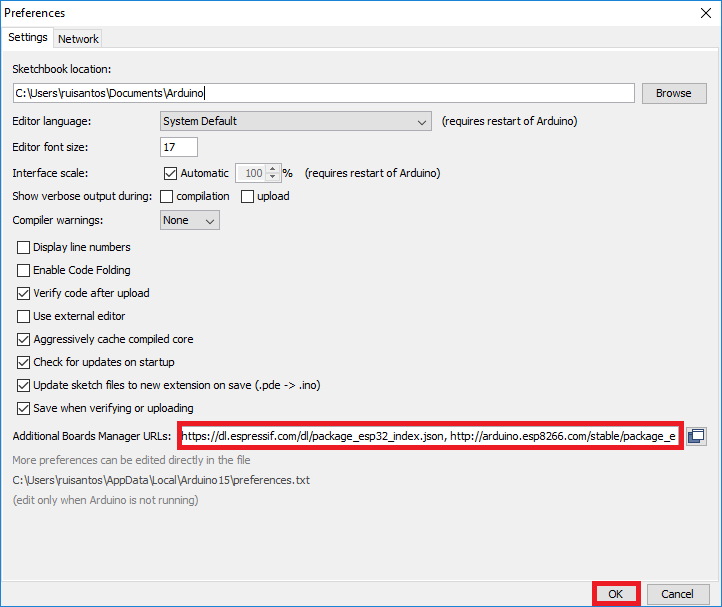
\includegraphics[width=1\textwidth]{figures/ArduinoIDE.png}
    \caption{Installing ESP32 board.}
    \label{fig:eessdff}
\end{figure}
    \item After that Go to Tools > Board > Boards Manager… and search for esp32 and install the latest version of it. See Figure~\ref{fig:eessdff}. 
    
      \begin{figure}[!htb]
    \centering
    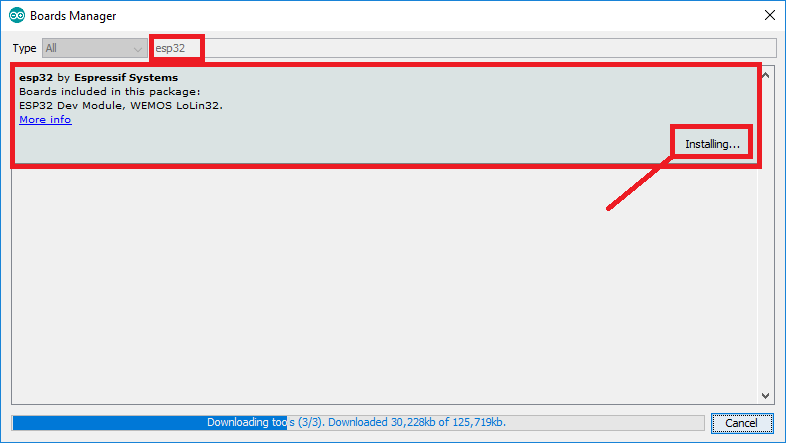
\includegraphics[width=1\textwidth]{figures/Arduinoboard.png}
    \caption{Installing ESP32 library.}
    \label{fig:eessdff}
\end{figure}
    \item It should be done. Now you can go to Tools > Board and select AI THINKER. 

 
\end{enumerate}


After that a number of libraries have to be installed in Arduino IDE: {\fontfamily{ccr}\selectfont Arduino\_JSON}, {\fontfamily{ccr}\selectfont Wifi}, {\fontfamily{ccr}\selectfont Wifi101}, {\fontfamily{ccr}\selectfont ESP32\_Mail\_Client} and {\fontfamily{ccr}\selectfont NTPClient}. 
By going to Tools > Manage Libraries you can install each one by one. 

The {\fontfamily{ccr}\selectfont Arduino} folder contains the firmware for Esp Eye and additional libraries. There are multiple Arduino files which show the step by step implementation. The last file to be uploaded in Arduino is: 

\framebox[1.1\width]{ Arduino/Final\_for\_submission/Final\_for\_submission.ino  } \par

\subsubsection{Registering Face IDs}
However in order to register face ids there is another sketch that needs to be uploaded to do that. Since the face ids are stored in flash then some changes need to be done in installation folder where Arduino IDE is installed in your computer. Before uploading the code for registration of faces there is a need to partition the flash to save little space for face Ids. Now you need to go to the partition folder which is typically located under this directory:
 
For windows downloaded Arduino Ide from Arduino Website:

\framebox{\parbox{\linewidth-2}{\itshape%
  C > Users > *your-user-name* > AppData > Local > Arduino15  > packages > esp32 > hardware > esp32 > 1.0.4 > tools > partitions }}
 

For Mac or Linux: 

\framebox{\parbox{\linewidth-2}{\itshape%
  Users > *your-user-name* > Library > Arduino15  > packages > esp32 > hardware > esp32 > 1.0.4 > tools > partitions }}

Now copy the file {\fontfamily{ccr}\selectfont faceid\_partitions.csv} found in the root directory of the repository and paste in the directory above. 

Now to let the board know about the partitioning there is a need to update the file {\fontfamily{ccr}\selectfont board.txt } located under the folder 1.0.4 which is in the two directories back from the partition folder and add the following lines: 

\framebox{\parbox{\linewidth-2}{\itshape%
esp32wrover.menu.PartitionScheme.faceid\_partition=Face Recognition (2621440 bytes with OTA)\par
esp32wrover.menu.PartitionScheme.faceid\_partition.build.partitions=faceid\_partitions

esp32wrover.menu.PartitionScheme.faceid\_partition.upload.maximum_size=2621440}}

Now use the {\fontfamily{ccr}\selectfont Enroll\_faces.ino } sketch to enroll face ids. After enrolling faces then upload the {\fontfamily{ccr}\selectfont Final\_for\_submission.ino } sketch. Finally, since the Esp Eye firmware acts as a station there is a need to update the SSID and password to connect to. 



\subsection{Hyperledger Fabric installation}

The Fabric network with implemented chaincode is located under {\fontfamily{ccr}\selectfont HLF } directory. At the time when we installed it HLF was the latest version but now it is no longer anymore and it is known as v2.1. 

We strongly encourage to have a look at the official HLB site for installation guidelines located at :

\framebox{\parbox{\linewidth-2}{\itshape%
https://hyperledger-fabric.readthedocs.io/en/release-2.1/getting\_started.html}}

\subsubsection{Prerequisites}
Before beginning the installation, there a number of prerequisites that need to be followed. Which can be seen also here in the link below:

\framebox{\parbox{\linewidth-2}{\itshape%
https://hyperledger-fabric.readthedocs.io/en/release-2.1/prereqs.html}}


\begin{enumerate}
    \item  The latest version of git for your OS
    \item The latest version of cURL
    \item The latest version of Docker and Docker Compose
\end{enumerate}

\subsubsection{Installing Hyperledger Fabric binaries and docker images}

\subsubsection{First method}
Now it is time to install Hyperledger Fabric binaries and docker images. For now there are two ways to do that, one way is to install a clean copy of HLP. Which can be seen in more detail in this link : 

\framebox{\parbox{\linewidth-2}{\itshape%
https://hyperledger-fabric.readthedocs.io/en/release-2.1/install.html}}

The github repository for HLF need to be cloned in a local directory, for macOS it has to use a location under /Users:

\framebox{\parbox{\linewidth-2}{\itshape%
git clone https://github.com/hyperledger/fabric-samples.git }}

Now it is the time to install binaries and docker images. To do so there should be a fabric-sample directory. In terminal under that directory execute the following command: 

\framebox{\parbox{\linewidth-2}{\itshape%
curl -sSL https://bit.ly/2ysbOFE | bash -s -- <fabric\_version> <fabric-ca\_version> <thirdparty\_version> }}



Which in our case would translate to v2.1 as below: 

\framebox{\parbox{\linewidth-2}{\itshape%
curl -sSL https://bit.ly/2ysbOFE | bash -s -- 2.1.1 1.4.7 0.4.20 }}


To pick up the docker containers without going to the path for each binary, it is recommended to do this: 

\framebox{\parbox{\linewidth-2}{\itshape%
export PATH=<path to the cloned HLF location>/bin:$PATH

}}




After that copy the {\fontfamily{ccr}\selectfont imagestore} folder under HLF and paste at the cloned copy of the Hyperledger Fabric. Under {\fontfamily{ccr}\selectfont chaincode} folder of HLF  we have the chaincode with a folder named imagestore copy that and paste under chaincode of the newly cloned Hyperledger Fabric under chaincode. It should by now be ready to run the project. 




\subsubsection{Second method}
The second way is to use the HLF directory of ours but a number of changes need to be done. First the {\fontfamily{ccr}\selectfont bin} folder has to be deleted because it contains the previous installed docker images. 

After that the binaries and docker images need to be installed locally. Similarly as above under the HLF directory the binaries need to be installed using the following command in Terminal: 

\framebox{\parbox{\linewidth-2}{\itshape%
curl -sSL https://bit.ly/2ysbOFE | bash -s -- 2.1.1 1.4.7 0.4.20 }}


To pick up the docker containers without going to the path for each binary, it is recommended to do this: 

\framebox{\parbox{\linewidth-2}{\itshape%
export PATH=<path to the cloned HLF location>/bin:$PATH

}} 
It is now expected that Hyperledger Fabric is installed and ready to be used. The two methods apply to all OS however the prerequisites may have to be installed using different package manager. 
For any issues it is recommended to follow the official HLF documentation links as above.





\subsubsection{Hyperledger Fabric application SDKs} 

Hyperledger Fabric provides a number of SDKs to support developing applications. Since we are using nodejs for the server, similarly nodejs SDK for fabric client is used. 
The prerequisites for nodejs SDK is that the following must be installed first: 

\begin{itemize}
    \item Node.js, version 10 is supported from 10.15.3 and higher
    \item  Node.js, version 12 is supported from 12.13.1 and higher
    \item npm tool version 6 or higher
\end{itemize}

To install the nodejs SDK:

\framebox{\parbox{\linewidth-2}{\itshape% 
npm install fabric-network
}} 

Hyperledger Fabric also offers a contract API for developing smart contacts. For nodejs use following command to install it:  

\framebox{\parbox{\linewidth-2}{\itshape% 
npm install --save fabric-contract-api
}} 

The main folders where our implementation lies in the source code of our project is {\fontfamily{ccr}\selectfont imagestore} folder. We strongly recommend to do :

\framebox{\parbox{\linewidth-2}{\itshape% 
npm install
}} 
under the folder
{\fontfamily{ccr}\selectfont /imagestore/javascript} where the nodejs server and HLF client are and under {\fontfamily{ccr}\selectfont /imagestore/frontend} which is the react web application.  


\subsubsection{Running Hyperledger Fabric}
To start the Fabric network, docker must be running. 
To start with in Terminal go to {\fontfamily{ccr}\selectfont imagestore} and do: 

\framebox{\parbox{\linewidth-2}{\itshape% 
./startNetwork.sh javascript
}}
And it should look like the Figure Figure~\ref{fig:eessdffsfsf}.

    \begin{figure}[!htb]
    \centering
    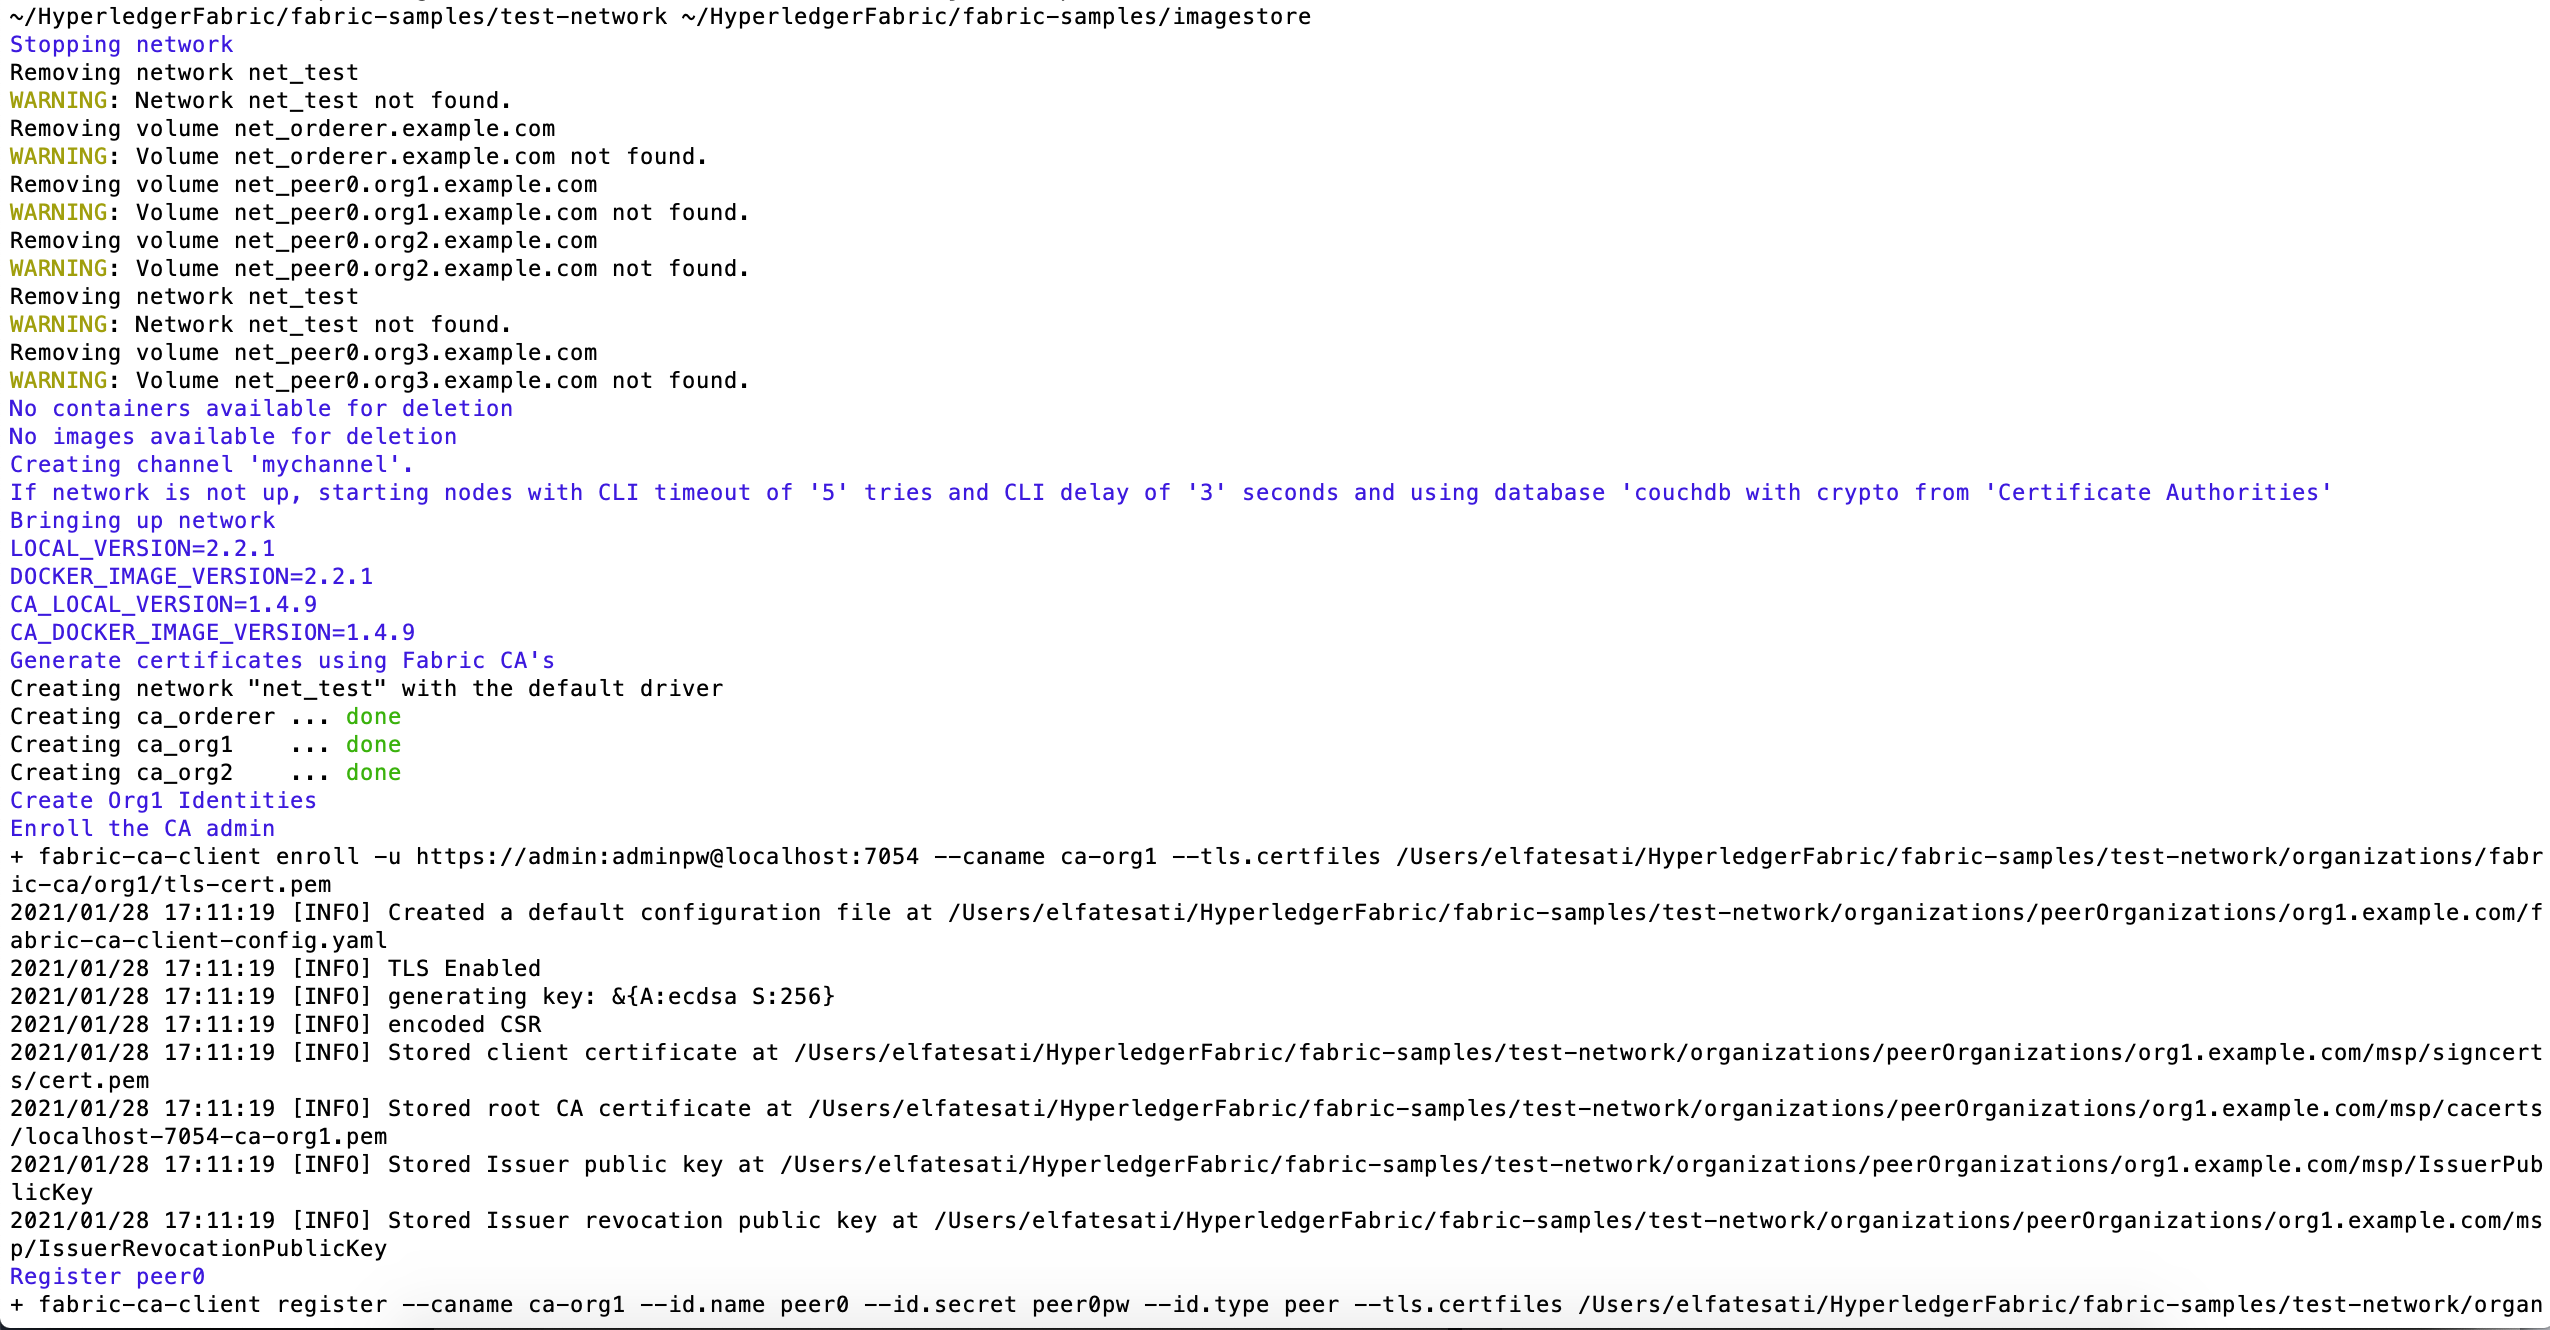
\includegraphics[width=1\textwidth]{figures/RunningHLF.png}
    \caption{ }
    \label{fig:eessdffsfsf}
\end{figure}
This script will start the network and docker containers, besides it will simultaneously deploy the smart contract specified in the chaincode. If you want to know more see the startNetwork.sh file. Basically it creates the network with 2 organisations and 2 ordering peers. The chaincode also gets deployed which is located under 
{\fontfamily{ccr}\selectfont /chaincode/imagestore/javascript/}.

The last step wow to create an Administrator and a user move to {\fontfamily{ccr}\selectfont /imagestore/javascript/} and run: 

\framebox{\parbox{\linewidth-2}{\itshape% 
node enrollAdmin.js
}}

\framebox{\parbox{\linewidth-2}{\itshape% 
node registerUser.js
}}


\subsection{Running the Web Application}

The web application is located under {\fontfamily{ccr}\selectfont /imagestore/frontnend}, cd into this folder and do : 
\framebox{\parbox{\linewidth-2}{\itshape% 
npm install
}}
\framebox{\parbox{\linewidth-2}{\itshape% 
npm start
}}

\subsection{Fabric Explorer}
Fabric Explorer is optional. To install it you can use the following link and it offers a number of options: 

\framebox{\parbox{\linewidth-2}{\itshape% 
https://github.com/hyperledger/blockchain-explorer
}}

We recommend installing it using docker. The Fabric Explorer container comes automatically when binaries are installed . First of all it assumes the Fabric network is already running. Under the root directory of the source of this project there is a folder named {\fontfamily{ccr}\selectfont Fabricexplorer} which holds the necessary files to make Explorer running. The file that should be updated is the {\fontfamily{ccr}\selectfont connection-profile/test-network.json}. In this file the {\fontfamily{ccr}\selectfont adminPrivateKey} has to be updated with the newly generated private key with location in Hyperledger Fabric: 



\framebox{\parbox{\linewidth-2}{\itshape% 
/peerOrganizations/org1.example.com/users/Admin@org1.example.com/msp/keystore
}}



\chapter{Contents of the CD}
The CD contains the following:

\begin{itemize}
    \item a folder with the Arduino source code
    \item a folder with the Arduino Libraries
    \item a folder for Hyperledger Fabric
    \item a folder with Web Application
    \item a folder with R Code
    \item a folder with Fabric Explorer
    \item a folder with the thesis source code and the final thesis pdf
 
\end{itemize}

\emph{All the above mentioned folders are available in a Zipped file.}




%\section{C-RAN for LoRa}\label{c-ran-for-lora}

An Arduino with a LoRa shield sends out packets over the air in an
interval. Some packets require an acknowledgment (ACK). If an ACK is
required, the Arduino waits for a certain amount of time for the ACK. If
the ACK arrives in time, the Arduino starts transmitting the next
packet. If not, the Arduino will resend the packet and again wait for
the ACK.

The RRH (Remote Radio Head) receives radio waves with a LimeSDR. The RRH
streams the IQ samples over the network the the BBU (Base Band Unit).

The BBU decodes the message. If the message says it require and ACK, the
BBU send out IQ samples of the ACK message over the network to the RRH
which transmits them back over the air to the Arduino.

\subsection{Run with Docker}\label{run-with-docker}

\begin{enumerate}
\def\labelenumi{\arabic{enumi}.}
\tightlist
\item
  Clone the repo
\item
  Go to the docker directory
\end{enumerate}

\subsubsection{\texorpdfstring{\textbf{\emph{Info}}}{Info}}\label{info}

\begin{itemize}
\tightlist
\item
  The container run in priviledged mode to easily access plugged in USB
  devices
\item
  The container run in network mode host (No NAT or Bridge has to be
  considered). This means the containers have the ip address of the host
  machine. If RRH and BBU run on different machines, find out their
  respective IP with \emph{ifconfig} and pass the address as arguments
  in the docker-compose.yml, see below.
\end{itemize}

\begin{center}\rule{0.5\linewidth}{\linethickness}\end{center}

\subsection{RRH}\label{rrh}

In the RRH directory run:

\begin{verbatim}
docker-compose up 
\end{verbatim}

This starts the Remote Radio Head. The RRH looks for a LimeSDR, it
prints errors if it cannot find one. You can plug one in after the
container has started and it should get detectet. By default it uses the
first LimeSDR it can find.

\subsubsection{Parameters}\label{parameters}

There are various parameters which you can specify in the
\emph{docker-compose.yml} file.

Run this to see what the possible params are:

\begin{verbatim}
./zero_mq_split_a.py -h
\end{verbatim}

Output:

\begin{verbatim}
Usage: zero_mq_split_a.py: [options]

Options:
  -h, --help            show this help message and exit
  --RX-device-serial=RX_DEVICE_SERIAL
                        Set RX_device_serial [default=]
  --TX-device-serial=TX_DEVICE_SERIAL
                        Set TX_device_serial [default=]
  --capture-freq=CAPTURE_FREQ
                        Set capture_freq [default=868.5M]
  --samp-rate=SAMP_RATE
                        Set samp_rate [default=1.0M]
  --zmq-address-iq-in=ZMQ_ADDRESS_IQ_IN
                        Set zmq_address_iq_in [default=tcp://127.0.0.1:5052]
  --zmq-address-iq-out=ZMQ_ADDRESS_IQ_OUT
                        Set zmq_address_iq_out [default=tcp://*:5051]
\end{verbatim}

\begin{longtable}[]{@{}ll@{}}
\toprule
\begin{minipage}[b]{0.18\columnwidth}\raggedright\strut
Param\strut
\end{minipage} & \begin{minipage}[b]{0.18\columnwidth}\raggedright\strut
Explanation\strut
\end{minipage}\tabularnewline
\midrule
\endhead
\begin{minipage}[t]{0.18\columnwidth}\raggedright\strut
RX-device-serial\strut
\end{minipage} & \begin{minipage}[t]{0.18\columnwidth}\raggedright\strut
By default, the program will use the first LimeSDR it can find for
receiving and transmitting signal. If you have two devices you can
specify which should receive by passing the device Serial (See section
\textbf{Help} for more info)\strut
\end{minipage}\tabularnewline
\begin{minipage}[t]{0.18\columnwidth}\raggedright\strut
TX-device-serial\strut
\end{minipage} & \begin{minipage}[t]{0.18\columnwidth}\raggedright\strut
By default, the program will use the first LimeSDR it can find for
receiving and transmitting signal. If you have two devices you can
specify which should transmit by passing the device Serial (See section
\textbf{Help} for more info)\strut
\end{minipage}\tabularnewline
\begin{minipage}[t]{0.18\columnwidth}\raggedright\strut
capture-freq\strut
\end{minipage} & \begin{minipage}[t]{0.18\columnwidth}\raggedright\strut
The frequency in Hz at which the RRH listens for signals. Default value
is 86850000\strut
\end{minipage}\tabularnewline
\begin{minipage}[t]{0.18\columnwidth}\raggedright\strut
samp-rate\strut
\end{minipage} & \begin{minipage}[t]{0.18\columnwidth}\raggedright\strut
How many samples per second. Default value is 1000000. Must be at least
double the bandwidth of the expected signal see \emph{Nyquist-Shannon
principle}\strut
\end{minipage}\tabularnewline
\begin{minipage}[t]{0.18\columnwidth}\raggedright\strut
zmq-address-iq-in\strut
\end{minipage} & \begin{minipage}[t]{0.18\columnwidth}\raggedright\strut
ZMQ address to which the RRH subscribes to receive an IQ samples stream
(from the BBU) to then send out (TX). Default value is
tcp://127.0.0.1:5052 meaning the IQ samples are expected to come from
localhost on port 5052. Normally RRH and BBU are on different devices
but on the same network\strut
\end{minipage}\tabularnewline
\begin{minipage}[t]{0.18\columnwidth}\raggedright\strut
--zmq-address-iq-out\strut
\end{minipage} & \begin{minipage}[t]{0.18\columnwidth}\raggedright\strut
ZMQ address on which the RRH streams out the IQ samples (to the BBU) it
receives (RX). Default is tcp://*:5051 meaning it publishes the stream
on all interface on port 5051\strut
\end{minipage}\tabularnewline
\bottomrule
\end{longtable}

\begin{center}\rule{0.5\linewidth}{\linethickness}\end{center}

To pass the parameters you have to specify them in the
docker-compose.yml

Example:

To pass a capture frequencey of 915M and a sample rate of 250k enter the
params in the following way in the command field:

\emph{docker-compose.yml}

\begin{verbatim}
version: '3'
services:
    rrh:
        build: .
        privileged: true
        network_mode: host
        volumes:
                - /dev/bus/usb:/dev/bus/usb
        command: ["--capture-freq", "915000000", "--samp_rate", "250000"]
\end{verbatim}

\begin{center}\rule{0.5\linewidth}{\linethickness}\end{center}

\subsection{BBU}\label{bbu}

The BBU has two components: * LoRa\_Decoder: receives a stream of IQ
samples from the RRH, decodes the LoRa signal and sends the decoded
message out on a UDP socket * LoRa\_Network\_Server: receives the
messages from that UDP socket and, depending on message content, streams
response IQ samples to the RRH or does not give a response

In the BBU directory run:

\begin{verbatim}
docker-compose up 
\end{verbatim}

This starts both components of the BBU

\subsubsection{Params}\label{params}

The LoRa\_Decoder has the following params:

\begin{verbatim}
Usage: zero_mq_split_b.py: [options]

Options:
  -h, --help            show this help message and exit
  --bandwidth=BANDWIDTH
                        Set bandwidth [default=125000]
  --capture-freq=CAPTURE_FREQ
                        Set capture_freq [default=868.5M]
  --decoded-out-port=DECODED_OUT_PORT
                        Set decoded_out_port [default=40868]
  --samp-rate=SAMP_RATE
                        Set samp_rate [default=1.0M]
  --spreading-factor=SPREADING_FACTOR
                        Set spreading_factor [default=12]
  --zmq-address-iq-in=ZMQ_ADDRESS_IQ_IN
                        Set zmq_address_iq_in [default=tcp://127.0.0.1:5051]
\end{verbatim}

\begin{longtable}[]{@{}ll@{}}
\toprule
\begin{minipage}[b]{0.18\columnwidth}\raggedright\strut
Param\strut
\end{minipage} & \begin{minipage}[b]{0.18\columnwidth}\raggedright\strut
Explanation\strut
\end{minipage}\tabularnewline
\midrule
\endhead
\begin{minipage}[t]{0.18\columnwidth}\raggedright\strut
bandwith\strut
\end{minipage} & \begin{minipage}[t]{0.18\columnwidth}\raggedright\strut
The bandwidth in Hz of the LoRa signal. Default is 125000.\strut
\end{minipage}\tabularnewline
\begin{minipage}[t]{0.18\columnwidth}\raggedright\strut
capture-freq\strut
\end{minipage} & \begin{minipage}[t]{0.18\columnwidth}\raggedright\strut
The frequency in Hz of the LoRa signal. The RRH of course must also
listen on this frequeny. Default is 868500000.\strut
\end{minipage}\tabularnewline
\begin{minipage}[t]{0.18\columnwidth}\raggedright\strut
decoded-out-port\strut
\end{minipage} & \begin{minipage}[t]{0.18\columnwidth}\raggedright\strut
On which port the decoded messages will be sent out. Localhost only. The
LoRa\_Network\_Server needs to be configured to listen on this port.
Default is 40868.\strut
\end{minipage}\tabularnewline
\begin{minipage}[t]{0.18\columnwidth}\raggedright\strut
samp-rate\strut
\end{minipage} & \begin{minipage}[t]{0.18\columnwidth}\raggedright\strut
How many samples per second to expect from the RRH. Default is
1000000\strut
\end{minipage}\tabularnewline
\begin{minipage}[t]{0.18\columnwidth}\raggedright\strut
spreading-factor\strut
\end{minipage} & \begin{minipage}[t]{0.18\columnwidth}\raggedright\strut
The spreading factor of the incoming LoRa signal. From {[}7-12{]}
inclusive. Default is 12\strut
\end{minipage}\tabularnewline
\begin{minipage}[t]{0.18\columnwidth}\raggedright\strut
--zmq-address-iq-in\strut
\end{minipage} & \begin{minipage}[t]{0.18\columnwidth}\raggedright\strut
ZMQ address to which the BBU subscribes to receive an IQ samples stream
(from the RRH) to decode. Default value is tcp://127.0.0.1:5051 meaning
the IQ samples are expected to come from localhost on port 5051.
Normally RRH and BBU are on different devices but on the same
network\strut
\end{minipage}\tabularnewline
\bottomrule
\end{longtable}

\begin{center}\rule{0.5\linewidth}{\linethickness}\end{center}

The LoRa\_Network\_Server has the following params:

\begin{verbatim}
usage: lora_socket_server.py [-h] [-o OUT_PORT] [-i INPUT_PORT]

Connect to udp port for receiving decoded LoRa signals, if an ACK is required
publish ACK iq samples via zmq socket for Remote Radio Head to receive and
send out (TX).

optional arguments:
  -h, --help            show this help message and exit
  -o OUT_PORT, --out-port OUT_PORT
                        zmq port to publish downstream (i.e ACK) iq samples
                        (default: 5052)
  -i INPUT_PORT, --input-port INPUT_PORT
                        UDP port to connect for receiving decoded lora
                        messages (default: 40868)

\end{verbatim}

\begin{longtable}[]{@{}ll@{}}
\toprule
\begin{minipage}[b]{0.18\columnwidth}\raggedright\strut
Param\strut
\end{minipage} & \begin{minipage}[b]{0.18\columnwidth}\raggedright\strut
Explanation\strut
\end{minipage}\tabularnewline
\midrule
\endhead
\begin{minipage}[t]{0.18\columnwidth}\raggedright\strut
out-port\strut
\end{minipage} & \begin{minipage}[t]{0.18\columnwidth}\raggedright\strut
Publish the response IQ samples on all interface on this port. Default
is 5052. (The response is 3 bytes long (``ACK'') and SF 12. This is
hardcoded for now)\strut
\end{minipage}\tabularnewline
\begin{minipage}[t]{0.18\columnwidth}\raggedright\strut
input-port\strut
\end{minipage} & \begin{minipage}[t]{0.18\columnwidth}\raggedright\strut
UDP port to receive the decoded messages sent by the LoRa\_Decoder.
Default is 40868\strut
\end{minipage}\tabularnewline
\bottomrule
\end{longtable}

\begin{center}\rule{0.5\linewidth}{\linethickness}\end{center}

To pass the parameters you have to specify them in the
docker-compose.yml file.

Example:

To have the LoRa\_Decoder send the decoded messages out on port 30300
and the Lora\_Network\_Server to listen on port 30300 accordingly pass
the arguments like below to the respective command field:

\emph{docker-compose.yml}

\begin{verbatim}
version: '3'
services:
        lora_decoder:
                build: ./LoRa_Decoder
                network_mode: host
                tty: true
                command: ["--decoded-out-port", "30300"]
        lora_network_server:
                build: ./LoRa_Network_Server
                network_mode: host
                tty: true
                command: ["--input-port", "30300"] 
\end{verbatim}

\subsection{LimeSDR}\label{limesdr}

\begin{itemize}
\tightlist
\item
  Plug in the antennas on the LimeSDR board on \emph{RX1\_L} and
  \emph{TX1\_1}
\end{itemize}

\subsection{Help}\label{help}

\begin{itemize}
\item
  LimeSDR calibration/gain error:
\item
  \href{https://wiki.myriadrf.org/Lime_Suite}{Download LimeSuite
  Toolkit} to calibrate the LimeSDR
\item
  LimeSDR find device serial:
\item
  With LimeSuite installed run \emph{LimeUtil --find}
\item
  Or run \emph{lsusb -v} and look for the LimeSDR device
\end{itemize}

\begin{center}\rule{0.5\linewidth}{\linethickness}\end{center}

\section{Arduino}\label{arduino}

\textbf{The arduino-lmic library is required
\href{https://github.com/matthijskooijman/arduino-lmic}{Instructions
here}}

\begin{enumerate}
\def\labelenumi{\arabic{enumi}.}
\tightlist
\item
  Go to the arduino directory.
\item
  Compile and upload the code to the arduino
\item
  The arduino runs the protocol in the manner described at the
  beginning.
\item
  It send packets with SF9 and expects the ACK response to be SF12 as
  well.
\item
  After 3 packets the arduino has finished.
\item
  Look at the Serial output for details. Baud rate 9600
\end{enumerate}

\textbf{Info}

PlatformIO was used to compile and upload the image to the arduino.

\begin{center}\rule{0.5\linewidth}{\linethickness}\end{center}

\subsection{Manual installation
Ubuntu}\label{manual-installation-ubuntu}

Visit this guide for
\href{https://wiki.myriadrf.org/Gr-limesdr_Plugin_for_GNURadio}{installing
LimeSDR Plugin for GNU Radio} for more detail. This guide only has the
short version.

Install dependencies for signal processing:

\begin{verbatim}
sudo apt-get update && sudo apt-get install -y gnuradio=3.7.11-10 libboost-all-dev swig git cmake software-properties-common \
libcppunit-1.14-0 libfftw3-bin libvolk1-bin liblog4cpp5v5 python libliquid1d libliquid-dev python-pip \
&& pip install numpy && pip install scipy
\end{verbatim}

Install LimeSuite

\begin{verbatim}
sudo add-apt-repository -y ppa:myriadrf/drivers && sudo apt-get update \
&& sudo apt-get install -y limesuite liblimesuite-dev limesuite-udev limesuite-images \
soapysdr-tools soapysdr-module-lms7
\end{verbatim}

Clone and install LimeSDR Plugin for GNU Radio:

\begin{verbatim}
git clone https://github.com/myriadrf/gr-limesdr && cd gr-limesdr && mkdir build && cd build && cmake .. && make && sudo make install && sudo ldconfig
\end{verbatim}

Clone and install rpp0's LoRa decoder for gnuradio

\begin{verbatim}
git clone https://github.com/rpp0/gr-lora.git && cd gr-lora && git checkout b1d38fab9032a52eaf31bf33a145df45fce7512f\
&& mkdir build && cd build \
&& cmake .. && make && sudo make install \
&& cd .. && rm -rf build \
&& git checkout -b encoder origin/encoder && git checkout 3c9a63f1d148592df2b715496c67ccbc2939ad0d \
&& mkdir build && cd build \
&& cmake .. && make && sudo make install && sudo ldconfig
\end{verbatim}

With pip for python2 install the zmq package:

\begin{verbatim}
pip install pyzmq==18.1.0
\end{verbatim}

Then open the \emph{zero\_mq\_split\_a.grc} and the
\emph{zero\_mq\_split\_b.grc} file in the docker/RRH directory resp. in
the docker/BBU/LoRa\_Decoder directory. Or run the
\emph{zero\_mq\_split\_a.py} resp. the \emph{zero\_mq\_split\_b.py}
script in those directories with your shell. Also run the
\emph{lora\_socket\_server.py} sript inside
docker/BBU/LoRa\_Network\_Server with your shell.

\section{Tools}\label{tools}

In the tools directory in the Encode and Decode directory are multiple
usefuls scripts for encoding and decoding lora without gnuradio

\begin{enumerate}
\def\labelenumi{\arabic{enumi}.}
\item
  First, after you recorded a signal trim the signal with a tool like
  audacity. Else if you want to visualize it with plot\_signal.py the
  signal is shrunk too much to make it fit in the plot.
\item
  After trimming, channelize the signal else the decoder cannot properly
  decode the signal. Run channelizer.py -h to see the options. It takes
  an signal recording via the --input-file option and outputs the
  channelized file as ``channelized.raw''. Don't forget to specify
  bandwidth and sample rate if they differ from the set default values.
\item
  The channelized signal can the be passed to the decoder. The decoder
  prints out the decoded signal and generates a csv file (words.csv)
  containing the words at each sample. Don't forget to specify bandwidth
  and sample rate etc if they differ from the set default values.
\item
  This csv file can be passed to plot\_signal.py which draws the signal
  and the words in the csv file to a pdf (rawframe.pdf). Don't forget to
  specify bandwidth and sample rate if they differ from the set default
  values.
\end{enumerate}

Use the encoder to generate samples for the test\_packet{[}{]} uint8
array in the code. The samples are written to the fiel ``output.bin''

Use the two scripts decoder\_build.sh and encoder\_build.sh to compile
the encode.cc and decode.cc files.

Use VsCode to open the directory ``Encode and Decode'' to have
predefiend debug configurations. The folder `.vscode' has been commited
in this repo.

All recorded uplink signals have been recorded with sample rate 1Million
and transmitted with a bandwidth of 125'000

The decoder only works for signals with an explicit header.




\end{document}
